\documentclass[twoside]{book}

% Packages required by doxygen
\usepackage{fixltx2e}
\usepackage{calc}
\usepackage{doxygen}
\usepackage[export]{adjustbox} % also loads graphicx
\usepackage{graphicx}
\usepackage[utf8]{inputenc}
\usepackage{makeidx}
\usepackage{multicol}
\usepackage{multirow}
\PassOptionsToPackage{warn}{textcomp}
\usepackage{textcomp}
\usepackage[nointegrals]{wasysym}
\usepackage[table]{xcolor}

% Font selection
\usepackage[T1]{fontenc}
\usepackage[scaled=.90]{helvet}
\usepackage{courier}
\usepackage{amssymb}
\usepackage{sectsty}
\renewcommand{\familydefault}{\sfdefault}
\allsectionsfont{%
  \fontseries{bc}\selectfont%
  \color{darkgray}%
}
\renewcommand{\DoxyLabelFont}{%
  \fontseries{bc}\selectfont%
  \color{darkgray}%
}
\newcommand{\+}{\discretionary{\mbox{\scriptsize$\hookleftarrow$}}{}{}}

% Page & text layout
\usepackage{geometry}
\geometry{%
  a4paper,%
  top=2.5cm,%
  bottom=2.5cm,%
  left=2.5cm,%
  right=2.5cm%
}
\tolerance=750
\hfuzz=15pt
\hbadness=750
\setlength{\emergencystretch}{15pt}
\setlength{\parindent}{0cm}
\setlength{\parskip}{3ex plus 2ex minus 2ex}
\makeatletter
\renewcommand{\paragraph}{%
  \@startsection{paragraph}{4}{0ex}{-1.0ex}{1.0ex}{%
    \normalfont\normalsize\bfseries\SS@parafont%
  }%
}
\renewcommand{\subparagraph}{%
  \@startsection{subparagraph}{5}{0ex}{-1.0ex}{1.0ex}{%
    \normalfont\normalsize\bfseries\SS@subparafont%
  }%
}
\makeatother

% Headers & footers
\usepackage{fancyhdr}
\pagestyle{fancyplain}
\fancyhead[LE]{\fancyplain{}{\bfseries\thepage}}
\fancyhead[CE]{\fancyplain{}{}}
\fancyhead[RE]{\fancyplain{}{\bfseries\leftmark}}
\fancyhead[LO]{\fancyplain{}{\bfseries\rightmark}}
\fancyhead[CO]{\fancyplain{}{}}
\fancyhead[RO]{\fancyplain{}{\bfseries\thepage}}
\fancyfoot[LE]{\fancyplain{}{}}
\fancyfoot[CE]{\fancyplain{}{}}
\fancyfoot[RE]{\fancyplain{}{\bfseries\scriptsize Generated by Doxygen }}
\fancyfoot[LO]{\fancyplain{}{\bfseries\scriptsize Generated by Doxygen }}
\fancyfoot[CO]{\fancyplain{}{}}
\fancyfoot[RO]{\fancyplain{}{}}
\renewcommand{\footrulewidth}{0.4pt}
\renewcommand{\chaptermark}[1]{%
  \markboth{#1}{}%
}
\renewcommand{\sectionmark}[1]{%
  \markright{\thesection\ #1}%
}

% Indices & bibliography
\usepackage{natbib}
\usepackage[titles]{tocloft}
\setcounter{tocdepth}{3}
\setcounter{secnumdepth}{5}
\makeindex

% Hyperlinks (required, but should be loaded last)
\usepackage{ifpdf}
\ifpdf
  \usepackage[pdftex,pagebackref=true]{hyperref}
\else
  \usepackage[ps2pdf,pagebackref=true]{hyperref}
\fi
\hypersetup{%
  colorlinks=true,%
  linkcolor=blue,%
  citecolor=blue,%
  unicode%
}

% Custom commands
\newcommand{\clearemptydoublepage}{%
  \newpage{\pagestyle{empty}\cleardoublepage}%
}

\usepackage{caption}
\captionsetup{labelsep=space,justification=centering,font={bf},singlelinecheck=off,skip=4pt,position=top}

%===== C O N T E N T S =====

\begin{document}

% Titlepage & ToC
\hypersetup{pageanchor=false,
             bookmarksnumbered=true,
             pdfencoding=unicode
            }
\pagenumbering{alph}
\begin{titlepage}
\vspace*{7cm}
\begin{center}%
{\Large Skypertawe }\\
\vspace*{1cm}
{\large Generated by Doxygen 1.8.13}\\
\end{center}
\end{titlepage}
\clearemptydoublepage
\pagenumbering{roman}
\tableofcontents
\clearemptydoublepage
\pagenumbering{arabic}
\hypersetup{pageanchor=true}

%--- Begin generated contents ---
\chapter{Hierarchical Index}
\section{Class Hierarchy}
This inheritance list is sorted roughly, but not completely, alphabetically\+:\begin{DoxyCompactList}
\item \contentsline{section}{Account}{\pageref{class_account}}{}
\item \contentsline{section}{B\+ST}{\pageref{class_b_s_t}}{}
\item \contentsline{section}{B\+S\+T\+Node}{\pageref{class_b_s_t_node}}{}
\item Comparable\begin{DoxyCompactList}
\item \contentsline{section}{Edge}{\pageref{class_edge}}{}
\end{DoxyCompactList}
\item \contentsline{section}{Graph}{\pageref{class_graph}}{}
\item \contentsline{section}{Line}{\pageref{class_line}}{}
\item \contentsline{section}{Main}{\pageref{class_main}}{}
\item \contentsline{section}{Message}{\pageref{class_message}}{}
\begin{DoxyCompactList}
\item \contentsline{section}{Text\+Message}{\pageref{class_text_message}}{}
\begin{DoxyCompactList}
\item \contentsline{section}{File\+Message}{\pageref{class_file_message}}{}
\item \contentsline{section}{U\+R\+L\+Message}{\pageref{class_u_r_l_message}}{}
\end{DoxyCompactList}
\end{DoxyCompactList}
\item \contentsline{section}{Read\+Write\+Account}{\pageref{class_read_write_account}}{}
\item \contentsline{section}{Read\+Write\+Friends}{\pageref{class_read_write_friends}}{}
\item \contentsline{section}{Read\+Write\+Message}{\pageref{class_read_write_message}}{}
\item \contentsline{section}{Vertex}{\pageref{class_vertex}}{}
\item J\+Frame\begin{DoxyCompactList}
\item \contentsline{section}{G\+UI}{\pageref{class_g_u_i}}{}
\begin{DoxyCompactList}
\item \contentsline{section}{Add\+Friend\+G\+UI}{\pageref{class_add_friend_g_u_i}}{}
\item \contentsline{section}{Collab\+Draw\+G\+UI}{\pageref{class_collab_draw_g_u_i}}{}
\item \contentsline{section}{Create\+Account\+G\+UI}{\pageref{class_create_account_g_u_i}}{}
\item \contentsline{section}{Home\+G\+UI}{\pageref{class_home_g_u_i}}{}
\item \contentsline{section}{Login\+G\+UI}{\pageref{class_login_g_u_i}}{}
\item \contentsline{section}{Message\+G\+U\+I2}{\pageref{class_message_g_u_i2}}{}
\item \contentsline{section}{Profile\+G\+UI}{\pageref{class_profile_g_u_i}}{}
\item \contentsline{section}{Select\+Draw\+G\+UI}{\pageref{class_select_draw_g_u_i}}{}
\item \contentsline{section}{Upload\+G\+UI}{\pageref{class_upload_g_u_i}}{}
\end{DoxyCompactList}
\end{DoxyCompactList}
\item J\+Panel\begin{DoxyCompactList}
\item \contentsline{section}{Drawing\+Panel}{\pageref{class_drawing_panel}}{}
\item \contentsline{section}{Profile\+Image\+Panel}{\pageref{class_profile_image_panel}}{}
\end{DoxyCompactList}
\end{DoxyCompactList}

\chapter{Class Index}
\section{Class List}
Here are the classes, structs, unions and interfaces with brief descriptions\+:\begin{DoxyCompactList}
\item\contentsline{section}{\hyperlink{class_account}{Account} }{\pageref{class_account}}{}
\item\contentsline{section}{\hyperlink{class_add_friend_g_u_i}{Add\+Friend\+G\+UI} }{\pageref{class_add_friend_g_u_i}}{}
\item\contentsline{section}{\hyperlink{class_b_s_t}{B\+ST} \\*Creates a binary search tree that allows \hyperlink{class_account}{Account} objects to be added as the elementsof \hyperlink{class_b_s_t_node}{B\+S\+T\+Node} objects }{\pageref{class_b_s_t}}{}
\item\contentsline{section}{\hyperlink{class_b_s_t_node}{B\+S\+T\+Node} \\*\hyperlink{class_b_s_t_node}{B\+S\+T\+Node} objects will be used to make up a \hyperlink{class_b_s_t}{B\+ST} }{\pageref{class_b_s_t_node}}{}
\item\contentsline{section}{\hyperlink{class_collab_draw_g_u_i}{Collab\+Draw\+G\+UI} }{\pageref{class_collab_draw_g_u_i}}{}
\item\contentsline{section}{\hyperlink{class_create_account_g_u_i}{Create\+Account\+G\+UI} }{\pageref{class_create_account_g_u_i}}{}
\item\contentsline{section}{\hyperlink{class_drawing_panel}{Drawing\+Panel} }{\pageref{class_drawing_panel}}{}
\item\contentsline{section}{\hyperlink{class_edge}{Edge} \\*Used in the \hyperlink{class_graph}{Graph} and \hyperlink{class_vertex}{Vertex} classes }{\pageref{class_edge}}{}
\item\contentsline{section}{\hyperlink{class_file_message}{File\+Message} }{\pageref{class_file_message}}{}
\item\contentsline{section}{\hyperlink{class_graph}{Graph} \\*Creates a graph using objects from the \hyperlink{class_vertex}{Vertex} class and objects from the \hyperlink{class_edge}{Edge} class }{\pageref{class_graph}}{}
\item\contentsline{section}{\hyperlink{class_g_u_i}{G\+UI} }{\pageref{class_g_u_i}}{}
\item\contentsline{section}{\hyperlink{class_home_g_u_i}{Home\+G\+UI} }{\pageref{class_home_g_u_i}}{}
\item\contentsline{section}{\hyperlink{class_line}{Line} }{\pageref{class_line}}{}
\item\contentsline{section}{\hyperlink{class_login_g_u_i}{Login\+G\+UI} }{\pageref{class_login_g_u_i}}{}
\item\contentsline{section}{\hyperlink{class_main}{Main} }{\pageref{class_main}}{}
\item\contentsline{section}{\hyperlink{class_message}{Message} }{\pageref{class_message}}{}
\item\contentsline{section}{\hyperlink{class_message_g_u_i2}{Message\+G\+U\+I2} }{\pageref{class_message_g_u_i2}}{}
\item\contentsline{section}{\hyperlink{class_profile_g_u_i}{Profile\+G\+UI} }{\pageref{class_profile_g_u_i}}{}
\item\contentsline{section}{\hyperlink{class_profile_image_panel}{Profile\+Image\+Panel} }{\pageref{class_profile_image_panel}}{}
\item\contentsline{section}{\hyperlink{class_read_write_account}{Read\+Write\+Account} }{\pageref{class_read_write_account}}{}
\item\contentsline{section}{\hyperlink{class_read_write_friends}{Read\+Write\+Friends} }{\pageref{class_read_write_friends}}{}
\item\contentsline{section}{\hyperlink{class_read_write_message}{Read\+Write\+Message} }{\pageref{class_read_write_message}}{}
\item\contentsline{section}{\hyperlink{class_select_draw_g_u_i}{Select\+Draw\+G\+UI} }{\pageref{class_select_draw_g_u_i}}{}
\item\contentsline{section}{\hyperlink{class_text_message}{Text\+Message} \\*Text\+Message.\+java }{\pageref{class_text_message}}{}
\item\contentsline{section}{\hyperlink{class_upload_g_u_i}{Upload\+G\+UI} }{\pageref{class_upload_g_u_i}}{}
\item\contentsline{section}{\hyperlink{class_u_r_l_message}{U\+R\+L\+Message} }{\pageref{class_u_r_l_message}}{}
\item\contentsline{section}{\hyperlink{class_vertex}{Vertex} \\*Will be used in the \hyperlink{class_graph}{Graph} and \hyperlink{class_edge}{Edge} classes }{\pageref{class_vertex}}{}
\end{DoxyCompactList}

\chapter{File Index}
\section{File List}
Here is a list of all documented files with brief descriptions\+:\begin{DoxyCompactList}
\item\contentsline{section}{readwrite/\hyperlink{_home_g_u_i_8java}{Home\+G\+U\+I.\+java} \\*Home screen for the Skypertawe application }{\pageref{_home_g_u_i_8java}}{}
\end{DoxyCompactList}

\chapter{Class Documentation}
\hypertarget{class_account}{}\section{Account Class Reference}
\label{class_account}\index{Account@{Account}}
\subsection*{Public Member Functions}
\begin{DoxyCompactItemize}
\item 
\mbox{\Hypertarget{class_account_a87f6c274e731792f3afb7d84179348f2}\label{class_account_a87f6c274e731792f3afb7d84179348f2}} 
{\bfseries Account} (String user, String first, String surname, String mobile, String birth, String city, int new\+Messages, String last\+Session, String img)
\item 
\mbox{\Hypertarget{class_account_aeb1a344ab7a43a65ed1e2327e3016e22}\label{class_account_aeb1a344ab7a43a65ed1e2327e3016e22}} 
void {\bfseries set\+Username} (String new\+Username)
\item 
\mbox{\Hypertarget{class_account_a9c231a2bbfa763ee161917582be7ca93}\label{class_account_a9c231a2bbfa763ee161917582be7ca93}} 
String {\bfseries get\+Username} ()
\item 
\mbox{\Hypertarget{class_account_a1dbd2d481b5a3bf8016c620bb0546285}\label{class_account_a1dbd2d481b5a3bf8016c620bb0546285}} 
void {\bfseries set\+First\+Name} (String new\+Firstname)
\item 
\mbox{\Hypertarget{class_account_a2fbf24827ade2497429bbd0bd3b92f3b}\label{class_account_a2fbf24827ade2497429bbd0bd3b92f3b}} 
String {\bfseries get\+First\+Name} ()
\item 
\mbox{\Hypertarget{class_account_a7a1f746590e16a91a05219190dffb6e9}\label{class_account_a7a1f746590e16a91a05219190dffb6e9}} 
void {\bfseries set\+Surname} (String new\+Surname)
\item 
\mbox{\Hypertarget{class_account_aad97893bafd1f37bd90b91dbd733a7b4}\label{class_account_aad97893bafd1f37bd90b91dbd733a7b4}} 
String {\bfseries get\+Surname} ()
\item 
\mbox{\Hypertarget{class_account_adc524e66e05cbaf086540011af3a9416}\label{class_account_adc524e66e05cbaf086540011af3a9416}} 
void {\bfseries set\+Mob\+Number} (String new\+Mob)
\item 
\mbox{\Hypertarget{class_account_a2af06a20ff55e26e1df6a2c138eec752}\label{class_account_a2af06a20ff55e26e1df6a2c138eec752}} 
String {\bfseries get\+Mobnumber} ()
\item 
\mbox{\Hypertarget{class_account_adb742c829886ec9f1c7a9781f8147144}\label{class_account_adb742c829886ec9f1c7a9781f8147144}} 
void {\bfseries set\+Birth\+Date} (String new\+Birth\+Date)
\item 
\mbox{\Hypertarget{class_account_a087047fb3e3026692e86b8a7eb9b90a1}\label{class_account_a087047fb3e3026692e86b8a7eb9b90a1}} 
String {\bfseries get\+Birth\+Date} ()
\item 
\mbox{\Hypertarget{class_account_a0eb38b6247bfe94fb5f785fe29b0d5e8}\label{class_account_a0eb38b6247bfe94fb5f785fe29b0d5e8}} 
void {\bfseries set\+City} (String new\+City)
\item 
\mbox{\Hypertarget{class_account_aa77cd9c25b58a8b332487c9033bcb3de}\label{class_account_aa77cd9c25b58a8b332487c9033bcb3de}} 
String {\bfseries get\+City} ()
\item 
\mbox{\Hypertarget{class_account_a50e909ccd2308b836a2eca9472986b1d}\label{class_account_a50e909ccd2308b836a2eca9472986b1d}} 
void {\bfseries set\+Num\+New\+Messages} (int new\+Messages)
\item 
\mbox{\Hypertarget{class_account_ab2243182691761884cd3a5e9672d9b3c}\label{class_account_ab2243182691761884cd3a5e9672d9b3c}} 
int {\bfseries get\+Num\+New\+Messages} ()
\item 
\mbox{\Hypertarget{class_account_af68df6233ed4805b65aea1c9e97e7127}\label{class_account_af68df6233ed4805b65aea1c9e97e7127}} 
void {\bfseries set\+Last\+Session} (String new\+Last\+Session)
\item 
\mbox{\Hypertarget{class_account_a2be799e4793ee03a7a4982d4f3abe35a}\label{class_account_a2be799e4793ee03a7a4982d4f3abe35a}} 
String {\bfseries get\+Last\+Session} ()
\item 
\mbox{\Hypertarget{class_account_ad27c4e798799d5f3b774db86f7ecd446}\label{class_account_ad27c4e798799d5f3b774db86f7ecd446}} 
void {\bfseries set\+Img\+Path} (String new\+Img\+Path)
\item 
\mbox{\Hypertarget{class_account_ad38a28ac366904c43deb3b9c7a1ba97b}\label{class_account_ad38a28ac366904c43deb3b9c7a1ba97b}} 
String {\bfseries get\+Img\+Path} ()
\end{DoxyCompactItemize}


The documentation for this class was generated from the following file\+:\begin{DoxyCompactItemize}
\item 
readwrite/Account.\+java\end{DoxyCompactItemize}

\hypertarget{class_add_friend_g_u_i}{}\section{Add\+Friend\+G\+UI Class Reference}
\label{class_add_friend_g_u_i}\index{Add\+Friend\+G\+UI@{Add\+Friend\+G\+UI}}
Inheritance diagram for Add\+Friend\+G\+UI\+:\begin{figure}[H]
\begin{center}
\leavevmode
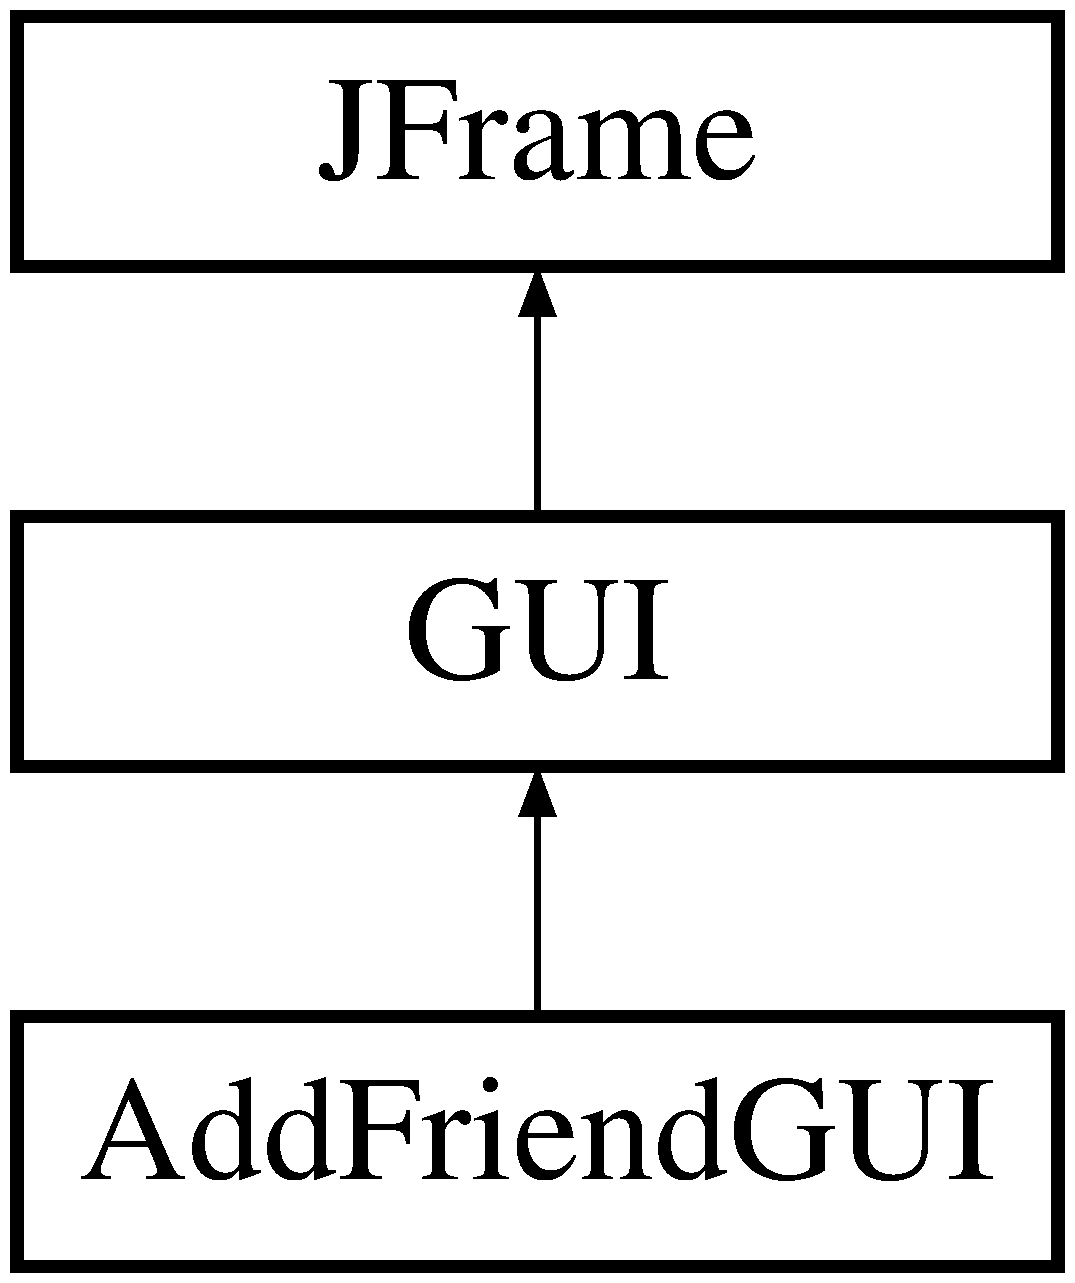
\includegraphics[height=3.000000cm]{class_add_friend_g_u_i}
\end{center}
\end{figure}
\subsection*{Public Member Functions}
\begin{DoxyCompactItemize}
\item 
\hyperlink{class_add_friend_g_u_i_ac389076c7c3445b2aa7bc426962b3d50}{Add\+Friend\+G\+UI} (\hyperlink{class_account}{Account} acc)  throws Exception 
\item 
void \hyperlink{class_add_friend_g_u_i_a5771685be048ff39517351ff19400104}{addfriendsetup} (\hyperlink{class_account}{Account} acc)  throws Exception
\begin{DoxyCompactList}\small\item\em Builds the screen and sets up the friendship when the add button is pressed. \end{DoxyCompactList}\end{DoxyCompactItemize}
\subsection*{Static Public Member Functions}
\begin{DoxyCompactItemize}
\item 
\mbox{\Hypertarget{class_add_friend_g_u_i_a7363bb35b73713abc94dc6e966b4b07e}\label{class_add_friend_g_u_i_a7363bb35b73713abc94dc6e966b4b07e}} 
static void \hyperlink{class_add_friend_g_u_i_a7363bb35b73713abc94dc6e966b4b07e}{main} (String\mbox{[}$\,$\mbox{]} args)  throws Exception 
\begin{DoxyCompactList}\small\item\em Implemented for testing purposes. \end{DoxyCompactList}\end{DoxyCompactItemize}


\subsection{Constructor \& Destructor Documentation}
\mbox{\Hypertarget{class_add_friend_g_u_i_ac389076c7c3445b2aa7bc426962b3d50}\label{class_add_friend_g_u_i_ac389076c7c3445b2aa7bc426962b3d50}} 
\index{Add\+Friend\+G\+UI@{Add\+Friend\+G\+UI}!Add\+Friend\+G\+UI@{Add\+Friend\+G\+UI}}
\index{Add\+Friend\+G\+UI@{Add\+Friend\+G\+UI}!Add\+Friend\+G\+UI@{Add\+Friend\+G\+UI}}
\subsubsection{\texorpdfstring{Add\+Friend\+G\+U\+I()}{AddFriendGUI()}}
{\footnotesize\ttfamily Add\+Friend\+G\+U\+I.\+Add\+Friend\+G\+UI (\begin{DoxyParamCaption}\item[{\hyperlink{class_account}{Account}}]{acc }\end{DoxyParamCaption}) throws Exception}


\begin{DoxyParams}{Parameters}
{\em acc} & the \hyperlink{class_account}{Account} currently logged in \\
\hline
\end{DoxyParams}


\subsection{Member Function Documentation}
\mbox{\Hypertarget{class_add_friend_g_u_i_a5771685be048ff39517351ff19400104}\label{class_add_friend_g_u_i_a5771685be048ff39517351ff19400104}} 
\index{Add\+Friend\+G\+UI@{Add\+Friend\+G\+UI}!addfriendsetup@{addfriendsetup}}
\index{addfriendsetup@{addfriendsetup}!Add\+Friend\+G\+UI@{Add\+Friend\+G\+UI}}
\subsubsection{\texorpdfstring{addfriendsetup()}{addfriendsetup()}}
{\footnotesize\ttfamily void Add\+Friend\+G\+U\+I.\+addfriendsetup (\begin{DoxyParamCaption}\item[{\hyperlink{class_account}{Account}}]{acc }\end{DoxyParamCaption}) throws Exception}



Builds the screen and sets up the friendship when the add button is pressed. 


\begin{DoxyParams}{Parameters}
{\em acc} & the \hyperlink{class_account}{Account} currently logged in \\
\hline
\end{DoxyParams}


The documentation for this class was generated from the following file\+:\begin{DoxyCompactItemize}
\item 
readwrite/Add\+Friend\+G\+U\+I.\+java\end{DoxyCompactItemize}

\hypertarget{class_b_s_t}{}\section{B\+ST Class Reference}
\label{class_b_s_t}\index{B\+ST@{B\+ST}}


The \hyperlink{class_b_s_t}{B\+ST} class creates a binary search tree that allows \hyperlink{class_account}{Account} objects to be added as the elementsof \hyperlink{class_b_s_t_node}{B\+S\+T\+Node} objects.  


\subsection*{Public Member Functions}
\begin{DoxyCompactItemize}
\item 
void \hyperlink{class_b_s_t_a618399aa893cac01fd09ee30329002da}{add\+Account} (\hyperlink{class_account}{Account} account)
\begin{DoxyCompactList}\small\item\em attempt to add an account to the tree \end{DoxyCompactList}\item 
Array\+List$<$ \hyperlink{class_account}{Account} $>$ \hyperlink{class_b_s_t_a6e9512f119e63d6179adeb1cbe53e668}{search\+Beginning\+With} (String search\+String)
\begin{DoxyCompactList}\small\item\em begin searching for users who\textquotesingle{}s username begins with the string being searched for \end{DoxyCompactList}\item 
void \hyperlink{class_b_s_t_a25a44d8679e06abada215f152dab7546}{print\+Alphabetical} (\hyperlink{class_b_s_t_node}{B\+S\+T\+Node} temp)
\begin{DoxyCompactList}\small\item\em print \hyperlink{class_account}{Account} usernames alphabetically \end{DoxyCompactList}\item 
Array\+List$<$ \hyperlink{class_account}{Account} $>$ \hyperlink{class_b_s_t_a8c2f9ab541fcf9566854b84ee5e9c97c}{get\+All\+Users} ()
\begin{DoxyCompactList}\small\item\em resets the search\+Result arraylist, calls a method to add all \hyperlink{class_account}{Account} objects to the arraylist, then returns the arraylist \end{DoxyCompactList}\item 
Array\+List$<$ \hyperlink{class_account}{Account} $>$ \hyperlink{class_b_s_t_a1474f85085f916fcc3c31ed639467ba6}{search\+Exact} (String search\+String)
\begin{DoxyCompactList}\small\item\em returns an array containing the one \hyperlink{class_account}{Account} that matches the search string exactly, empty if no match \end{DoxyCompactList}\item 
void \hyperlink{class_b_s_t_a2241cab2084ec74baea6feef5cf2df34}{perform\+Exact\+Search} (String search\+String, \hyperlink{class_b_s_t_node}{B\+S\+T\+Node} temp)
\begin{DoxyCompactList}\small\item\em performs the search for an exact match \end{DoxyCompactList}\item 
Array\+List$<$ \hyperlink{class_account}{Account} $>$ \hyperlink{class_b_s_t_a540417596be03377db2b2e86bfa29187}{search\+Contains} (String search\+String)
\begin{DoxyCompactList}\small\item\em resets the search\+Result arraylist, calls method to perform search, returns arraylist of \hyperlink{class_account}{Account} objects that contain the string \end{DoxyCompactList}\item 
void \hyperlink{class_b_s_t_a9bc75db08a0e8fe2bd80f3c5c7c59205}{add\+Accounts\+From\+Array\+List} (Array\+List$<$ \hyperlink{class_account}{Account} $>$ accounts)
\begin{DoxyCompactList}\small\item\em add accounts from an Array\+List$<$\+Account$>$ to the \hyperlink{class_b_s_t}{B\+ST} \end{DoxyCompactList}\item 
int \hyperlink{class_b_s_t_a7efc306d687afb24a2c79bdd15c2e1fd}{get\+Number\+Nodes} ()
\begin{DoxyCompactList}\small\item\em getter for number of nodes \end{DoxyCompactList}\item 
\hyperlink{class_b_s_t_node}{B\+S\+T\+Node} \hyperlink{class_b_s_t_a5d06adaf42f8e1d7f032a1b3be4cd813}{get\+Root} ()
\begin{DoxyCompactList}\small\item\em getter for the root of the tree \end{DoxyCompactList}\end{DoxyCompactItemize}


\subsection{Detailed Description}
The \hyperlink{class_b_s_t}{B\+ST} class creates a binary search tree that allows \hyperlink{class_account}{Account} objects to be added as the elementsof \hyperlink{class_b_s_t_node}{B\+S\+T\+Node} objects. 

\hyperlink{class_b_s_t}{B\+ST} has 4 different ways to retrieve \hyperlink{class_account}{Account} objects from the tree.

\begin{DoxyAuthor}{Author}
830169 
\end{DoxyAuthor}
\begin{DoxyVersion}{Version}
1.\+0 
\end{DoxyVersion}


\subsection{Member Function Documentation}
\mbox{\Hypertarget{class_b_s_t_a618399aa893cac01fd09ee30329002da}\label{class_b_s_t_a618399aa893cac01fd09ee30329002da}} 
\index{B\+ST@{B\+ST}!add\+Account@{add\+Account}}
\index{add\+Account@{add\+Account}!B\+ST@{B\+ST}}
\subsubsection{\texorpdfstring{add\+Account()}{addAccount()}}
{\footnotesize\ttfamily void B\+S\+T.\+add\+Account (\begin{DoxyParamCaption}\item[{\hyperlink{class_account}{Account}}]{account }\end{DoxyParamCaption})}



attempt to add an account to the tree 


\begin{DoxyParams}{Parameters}
{\em account} & the account to add to the tree \\
\hline
\end{DoxyParams}
\mbox{\Hypertarget{class_b_s_t_a9bc75db08a0e8fe2bd80f3c5c7c59205}\label{class_b_s_t_a9bc75db08a0e8fe2bd80f3c5c7c59205}} 
\index{B\+ST@{B\+ST}!add\+Accounts\+From\+Array\+List@{add\+Accounts\+From\+Array\+List}}
\index{add\+Accounts\+From\+Array\+List@{add\+Accounts\+From\+Array\+List}!B\+ST@{B\+ST}}
\subsubsection{\texorpdfstring{add\+Accounts\+From\+Array\+List()}{addAccountsFromArrayList()}}
{\footnotesize\ttfamily void B\+S\+T.\+add\+Accounts\+From\+Array\+List (\begin{DoxyParamCaption}\item[{Array\+List$<$ \hyperlink{class_account}{Account} $>$}]{accounts }\end{DoxyParamCaption})}



add accounts from an Array\+List$<$\+Account$>$ to the \hyperlink{class_b_s_t}{B\+ST} 


\begin{DoxyParams}{Parameters}
{\em accounts} & arraylist of \hyperlink{class_account}{Account} objects to be added to the tree \\
\hline
\end{DoxyParams}
\mbox{\Hypertarget{class_b_s_t_a8c2f9ab541fcf9566854b84ee5e9c97c}\label{class_b_s_t_a8c2f9ab541fcf9566854b84ee5e9c97c}} 
\index{B\+ST@{B\+ST}!get\+All\+Users@{get\+All\+Users}}
\index{get\+All\+Users@{get\+All\+Users}!B\+ST@{B\+ST}}
\subsubsection{\texorpdfstring{get\+All\+Users()}{getAllUsers()}}
{\footnotesize\ttfamily Array\+List$<$\hyperlink{class_account}{Account}$>$ B\+S\+T.\+get\+All\+Users (\begin{DoxyParamCaption}{ }\end{DoxyParamCaption})}



resets the search\+Result arraylist, calls a method to add all \hyperlink{class_account}{Account} objects to the arraylist, then returns the arraylist 

\begin{DoxyReturn}{Returns}
arraylist of all \hyperlink{class_account}{Account} objects in the tree, ordered alphabetically by username 
\end{DoxyReturn}
\mbox{\Hypertarget{class_b_s_t_a7efc306d687afb24a2c79bdd15c2e1fd}\label{class_b_s_t_a7efc306d687afb24a2c79bdd15c2e1fd}} 
\index{B\+ST@{B\+ST}!get\+Number\+Nodes@{get\+Number\+Nodes}}
\index{get\+Number\+Nodes@{get\+Number\+Nodes}!B\+ST@{B\+ST}}
\subsubsection{\texorpdfstring{get\+Number\+Nodes()}{getNumberNodes()}}
{\footnotesize\ttfamily int B\+S\+T.\+get\+Number\+Nodes (\begin{DoxyParamCaption}{ }\end{DoxyParamCaption})}



getter for number of nodes 

\begin{DoxyReturn}{Returns}
the number of nodes in the tree 
\end{DoxyReturn}
\mbox{\Hypertarget{class_b_s_t_a5d06adaf42f8e1d7f032a1b3be4cd813}\label{class_b_s_t_a5d06adaf42f8e1d7f032a1b3be4cd813}} 
\index{B\+ST@{B\+ST}!get\+Root@{get\+Root}}
\index{get\+Root@{get\+Root}!B\+ST@{B\+ST}}
\subsubsection{\texorpdfstring{get\+Root()}{getRoot()}}
{\footnotesize\ttfamily \hyperlink{class_b_s_t_node}{B\+S\+T\+Node} B\+S\+T.\+get\+Root (\begin{DoxyParamCaption}{ }\end{DoxyParamCaption})}



getter for the root of the tree 

\begin{DoxyReturn}{Returns}
a reference to the root of the tree 
\end{DoxyReturn}
\mbox{\Hypertarget{class_b_s_t_a2241cab2084ec74baea6feef5cf2df34}\label{class_b_s_t_a2241cab2084ec74baea6feef5cf2df34}} 
\index{B\+ST@{B\+ST}!perform\+Exact\+Search@{perform\+Exact\+Search}}
\index{perform\+Exact\+Search@{perform\+Exact\+Search}!B\+ST@{B\+ST}}
\subsubsection{\texorpdfstring{perform\+Exact\+Search()}{performExactSearch()}}
{\footnotesize\ttfamily void B\+S\+T.\+perform\+Exact\+Search (\begin{DoxyParamCaption}\item[{String}]{search\+String,  }\item[{\hyperlink{class_b_s_t_node}{B\+S\+T\+Node}}]{temp }\end{DoxyParamCaption})}



performs the search for an exact match 


\begin{DoxyParams}{Parameters}
{\em search\+String} & string being searched for \\
\hline
{\em temp} & the node reference that allows the tree to recursively call the method to traverse the tree \\
\hline
\end{DoxyParams}
\mbox{\Hypertarget{class_b_s_t_a25a44d8679e06abada215f152dab7546}\label{class_b_s_t_a25a44d8679e06abada215f152dab7546}} 
\index{B\+ST@{B\+ST}!print\+Alphabetical@{print\+Alphabetical}}
\index{print\+Alphabetical@{print\+Alphabetical}!B\+ST@{B\+ST}}
\subsubsection{\texorpdfstring{print\+Alphabetical()}{printAlphabetical()}}
{\footnotesize\ttfamily void B\+S\+T.\+print\+Alphabetical (\begin{DoxyParamCaption}\item[{\hyperlink{class_b_s_t_node}{B\+S\+T\+Node}}]{temp }\end{DoxyParamCaption})}



print \hyperlink{class_account}{Account} usernames alphabetically 


\begin{DoxyParams}{Parameters}
{\em temp} & the node reference that allows the tree to recursively call the method to traverse the tree \\
\hline
\end{DoxyParams}
\mbox{\Hypertarget{class_b_s_t_a6e9512f119e63d6179adeb1cbe53e668}\label{class_b_s_t_a6e9512f119e63d6179adeb1cbe53e668}} 
\index{B\+ST@{B\+ST}!search\+Beginning\+With@{search\+Beginning\+With}}
\index{search\+Beginning\+With@{search\+Beginning\+With}!B\+ST@{B\+ST}}
\subsubsection{\texorpdfstring{search\+Beginning\+With()}{searchBeginningWith()}}
{\footnotesize\ttfamily Array\+List$<$\hyperlink{class_account}{Account}$>$ B\+S\+T.\+search\+Beginning\+With (\begin{DoxyParamCaption}\item[{String}]{search\+String }\end{DoxyParamCaption})}



begin searching for users who\textquotesingle{}s username begins with the string being searched for 


\begin{DoxyParams}{Parameters}
{\em search\+String} & the string to search for \\
\hline
\end{DoxyParams}
\begin{DoxyReturn}{Returns}
the arraylist of accounts that were found by the search 
\end{DoxyReturn}
\mbox{\Hypertarget{class_b_s_t_a540417596be03377db2b2e86bfa29187}\label{class_b_s_t_a540417596be03377db2b2e86bfa29187}} 
\index{B\+ST@{B\+ST}!search\+Contains@{search\+Contains}}
\index{search\+Contains@{search\+Contains}!B\+ST@{B\+ST}}
\subsubsection{\texorpdfstring{search\+Contains()}{searchContains()}}
{\footnotesize\ttfamily Array\+List$<$\hyperlink{class_account}{Account}$>$ B\+S\+T.\+search\+Contains (\begin{DoxyParamCaption}\item[{String}]{search\+String }\end{DoxyParamCaption})}



resets the search\+Result arraylist, calls method to perform search, returns arraylist of \hyperlink{class_account}{Account} objects that contain the string 


\begin{DoxyParams}{Parameters}
{\em search\+String} & string being searched for \\
\hline
\end{DoxyParams}
\begin{DoxyReturn}{Returns}
arraylist of \hyperlink{class_account}{Account} objects who\textquotesingle{}s usernames contain the search string 
\end{DoxyReturn}
\mbox{\Hypertarget{class_b_s_t_a1474f85085f916fcc3c31ed639467ba6}\label{class_b_s_t_a1474f85085f916fcc3c31ed639467ba6}} 
\index{B\+ST@{B\+ST}!search\+Exact@{search\+Exact}}
\index{search\+Exact@{search\+Exact}!B\+ST@{B\+ST}}
\subsubsection{\texorpdfstring{search\+Exact()}{searchExact()}}
{\footnotesize\ttfamily Array\+List$<$\hyperlink{class_account}{Account}$>$ B\+S\+T.\+search\+Exact (\begin{DoxyParamCaption}\item[{String}]{search\+String }\end{DoxyParamCaption})}



returns an array containing the one \hyperlink{class_account}{Account} that matches the search string exactly, empty if no match 


\begin{DoxyParams}{Parameters}
{\em search\+String} & string being searched for \\
\hline
\end{DoxyParams}
\begin{DoxyReturn}{Returns}
arraylist with one \hyperlink{class_account}{Account} that matched the search string exactly, or empty if no match 
\end{DoxyReturn}


The documentation for this class was generated from the following file\+:\begin{DoxyCompactItemize}
\item 
readwrite/B\+S\+T.\+java\end{DoxyCompactItemize}

\hypertarget{class_b_s_t_node}{}\section{B\+S\+T\+Node Class Reference}
\label{class_b_s_t_node}\index{B\+S\+T\+Node@{B\+S\+T\+Node}}


the \hyperlink{class_b_s_t_node}{B\+S\+T\+Node} objects will be used to make up a \hyperlink{class_b_s_t}{B\+ST}.  


\subsection*{Public Member Functions}
\begin{DoxyCompactItemize}
\item 
\hyperlink{class_b_s_t_node_aaa051f6a85f1cbc75800579027bce3cf}{B\+S\+T\+Node} (\hyperlink{class_account}{Account} account)
\begin{DoxyCompactList}\small\item\em constructor for \hyperlink{class_b_s_t_node}{B\+S\+T\+Node} \end{DoxyCompactList}\item 
void \hyperlink{class_b_s_t_node_a1e2bfb150abc14665b512b10854b4dd4}{set\+Account} (\hyperlink{class_account}{Account} account)
\begin{DoxyCompactList}\small\item\em setter for the element of the \hyperlink{class_b_s_t_node}{B\+S\+T\+Node} \end{DoxyCompactList}\item 
\hyperlink{class_account}{Account} \hyperlink{class_b_s_t_node_a182e6ee7245ac0f1f2911fd0118625e5}{get\+Account} ()
\begin{DoxyCompactList}\small\item\em getter for the \hyperlink{class_account}{Account} that the element attribute references \end{DoxyCompactList}\item 
\hyperlink{class_b_s_t_node}{B\+S\+T\+Node} \hyperlink{class_b_s_t_node_aa54083ff3ae616311f577131f4b66e64}{get\+Left} ()
\begin{DoxyCompactList}\small\item\em getter for the node to the left of this node \end{DoxyCompactList}\item 
\hyperlink{class_b_s_t_node}{B\+S\+T\+Node} \hyperlink{class_b_s_t_node_a986cf72ed573103cf1f27234970eda98}{get\+Right} ()
\begin{DoxyCompactList}\small\item\em getter for node to the right of this node \end{DoxyCompactList}\item 
void \hyperlink{class_b_s_t_node_a5bb0ba5ce7d5663bd4b17809e14d4a6c}{set\+Left} (\hyperlink{class_b_s_t_node}{B\+S\+T\+Node} l)
\begin{DoxyCompactList}\small\item\em setter for the left node \end{DoxyCompactList}\item 
void \hyperlink{class_b_s_t_node_a945445bf310d0f27f15eff0726c01f03}{set\+Right} (\hyperlink{class_b_s_t_node}{B\+S\+T\+Node} r)
\begin{DoxyCompactList}\small\item\em setter for the right node \end{DoxyCompactList}\end{DoxyCompactItemize}


\subsection{Detailed Description}
the \hyperlink{class_b_s_t_node}{B\+S\+T\+Node} objects will be used to make up a \hyperlink{class_b_s_t}{B\+ST}. 

the B\+S\+T\+Nodes contain an element of type \hyperlink{class_account}{Account}, and a left/right references of type \hyperlink{class_b_s_t_node}{B\+S\+T\+Node}

\begin{DoxyAuthor}{Author}
830169 
\end{DoxyAuthor}
\begin{DoxyVersion}{Version}
1.\+0 
\end{DoxyVersion}


\subsection{Constructor \& Destructor Documentation}
\mbox{\Hypertarget{class_b_s_t_node_aaa051f6a85f1cbc75800579027bce3cf}\label{class_b_s_t_node_aaa051f6a85f1cbc75800579027bce3cf}} 
\index{B\+S\+T\+Node@{B\+S\+T\+Node}!B\+S\+T\+Node@{B\+S\+T\+Node}}
\index{B\+S\+T\+Node@{B\+S\+T\+Node}!B\+S\+T\+Node@{B\+S\+T\+Node}}
\subsubsection{\texorpdfstring{B\+S\+T\+Node()}{BSTNode()}}
{\footnotesize\ttfamily B\+S\+T\+Node.\+B\+S\+T\+Node (\begin{DoxyParamCaption}\item[{\hyperlink{class_account}{Account}}]{account }\end{DoxyParamCaption})}



constructor for \hyperlink{class_b_s_t_node}{B\+S\+T\+Node} 


\begin{DoxyParams}{Parameters}
{\em account} & the account that the element will reference \\
\hline
\end{DoxyParams}


\subsection{Member Function Documentation}
\mbox{\Hypertarget{class_b_s_t_node_a182e6ee7245ac0f1f2911fd0118625e5}\label{class_b_s_t_node_a182e6ee7245ac0f1f2911fd0118625e5}} 
\index{B\+S\+T\+Node@{B\+S\+T\+Node}!get\+Account@{get\+Account}}
\index{get\+Account@{get\+Account}!B\+S\+T\+Node@{B\+S\+T\+Node}}
\subsubsection{\texorpdfstring{get\+Account()}{getAccount()}}
{\footnotesize\ttfamily \hyperlink{class_account}{Account} B\+S\+T\+Node.\+get\+Account (\begin{DoxyParamCaption}{ }\end{DoxyParamCaption})}



getter for the \hyperlink{class_account}{Account} that the element attribute references 

\begin{DoxyReturn}{Returns}
the \hyperlink{class_account}{Account} object of this node 
\end{DoxyReturn}
\mbox{\Hypertarget{class_b_s_t_node_aa54083ff3ae616311f577131f4b66e64}\label{class_b_s_t_node_aa54083ff3ae616311f577131f4b66e64}} 
\index{B\+S\+T\+Node@{B\+S\+T\+Node}!get\+Left@{get\+Left}}
\index{get\+Left@{get\+Left}!B\+S\+T\+Node@{B\+S\+T\+Node}}
\subsubsection{\texorpdfstring{get\+Left()}{getLeft()}}
{\footnotesize\ttfamily \hyperlink{class_b_s_t_node}{B\+S\+T\+Node} B\+S\+T\+Node.\+get\+Left (\begin{DoxyParamCaption}{ }\end{DoxyParamCaption})}



getter for the node to the left of this node 

\begin{DoxyReturn}{Returns}
reference to the left node 
\end{DoxyReturn}
\mbox{\Hypertarget{class_b_s_t_node_a986cf72ed573103cf1f27234970eda98}\label{class_b_s_t_node_a986cf72ed573103cf1f27234970eda98}} 
\index{B\+S\+T\+Node@{B\+S\+T\+Node}!get\+Right@{get\+Right}}
\index{get\+Right@{get\+Right}!B\+S\+T\+Node@{B\+S\+T\+Node}}
\subsubsection{\texorpdfstring{get\+Right()}{getRight()}}
{\footnotesize\ttfamily \hyperlink{class_b_s_t_node}{B\+S\+T\+Node} B\+S\+T\+Node.\+get\+Right (\begin{DoxyParamCaption}{ }\end{DoxyParamCaption})}



getter for node to the right of this node 

\begin{DoxyReturn}{Returns}
reference to the right node 
\end{DoxyReturn}
\mbox{\Hypertarget{class_b_s_t_node_a1e2bfb150abc14665b512b10854b4dd4}\label{class_b_s_t_node_a1e2bfb150abc14665b512b10854b4dd4}} 
\index{B\+S\+T\+Node@{B\+S\+T\+Node}!set\+Account@{set\+Account}}
\index{set\+Account@{set\+Account}!B\+S\+T\+Node@{B\+S\+T\+Node}}
\subsubsection{\texorpdfstring{set\+Account()}{setAccount()}}
{\footnotesize\ttfamily void B\+S\+T\+Node.\+set\+Account (\begin{DoxyParamCaption}\item[{\hyperlink{class_account}{Account}}]{account }\end{DoxyParamCaption})}



setter for the element of the \hyperlink{class_b_s_t_node}{B\+S\+T\+Node} 


\begin{DoxyParams}{Parameters}
{\em account} & the new \hyperlink{class_account}{Account} that the element attribute will reference \\
\hline
\end{DoxyParams}
\mbox{\Hypertarget{class_b_s_t_node_a5bb0ba5ce7d5663bd4b17809e14d4a6c}\label{class_b_s_t_node_a5bb0ba5ce7d5663bd4b17809e14d4a6c}} 
\index{B\+S\+T\+Node@{B\+S\+T\+Node}!set\+Left@{set\+Left}}
\index{set\+Left@{set\+Left}!B\+S\+T\+Node@{B\+S\+T\+Node}}
\subsubsection{\texorpdfstring{set\+Left()}{setLeft()}}
{\footnotesize\ttfamily void B\+S\+T\+Node.\+set\+Left (\begin{DoxyParamCaption}\item[{\hyperlink{class_b_s_t_node}{B\+S\+T\+Node}}]{l }\end{DoxyParamCaption})}



setter for the left node 


\begin{DoxyParams}{Parameters}
{\em l} & reference to the new left node \\
\hline
\end{DoxyParams}
\mbox{\Hypertarget{class_b_s_t_node_a945445bf310d0f27f15eff0726c01f03}\label{class_b_s_t_node_a945445bf310d0f27f15eff0726c01f03}} 
\index{B\+S\+T\+Node@{B\+S\+T\+Node}!set\+Right@{set\+Right}}
\index{set\+Right@{set\+Right}!B\+S\+T\+Node@{B\+S\+T\+Node}}
\subsubsection{\texorpdfstring{set\+Right()}{setRight()}}
{\footnotesize\ttfamily void B\+S\+T\+Node.\+set\+Right (\begin{DoxyParamCaption}\item[{\hyperlink{class_b_s_t_node}{B\+S\+T\+Node}}]{r }\end{DoxyParamCaption})}



setter for the right node 


\begin{DoxyParams}{Parameters}
{\em r} & reference to the new right node \\
\hline
\end{DoxyParams}


The documentation for this class was generated from the following file\+:\begin{DoxyCompactItemize}
\item 
readwrite/B\+S\+T\+Node.\+java\end{DoxyCompactItemize}

\hypertarget{class_collab_draw_g_u_i}{}\section{Collab\+Draw\+G\+UI Class Reference}
\label{class_collab_draw_g_u_i}\index{Collab\+Draw\+G\+UI@{Collab\+Draw\+G\+UI}}
Inheritance diagram for Collab\+Draw\+G\+UI\+:\begin{figure}[H]
\begin{center}
\leavevmode
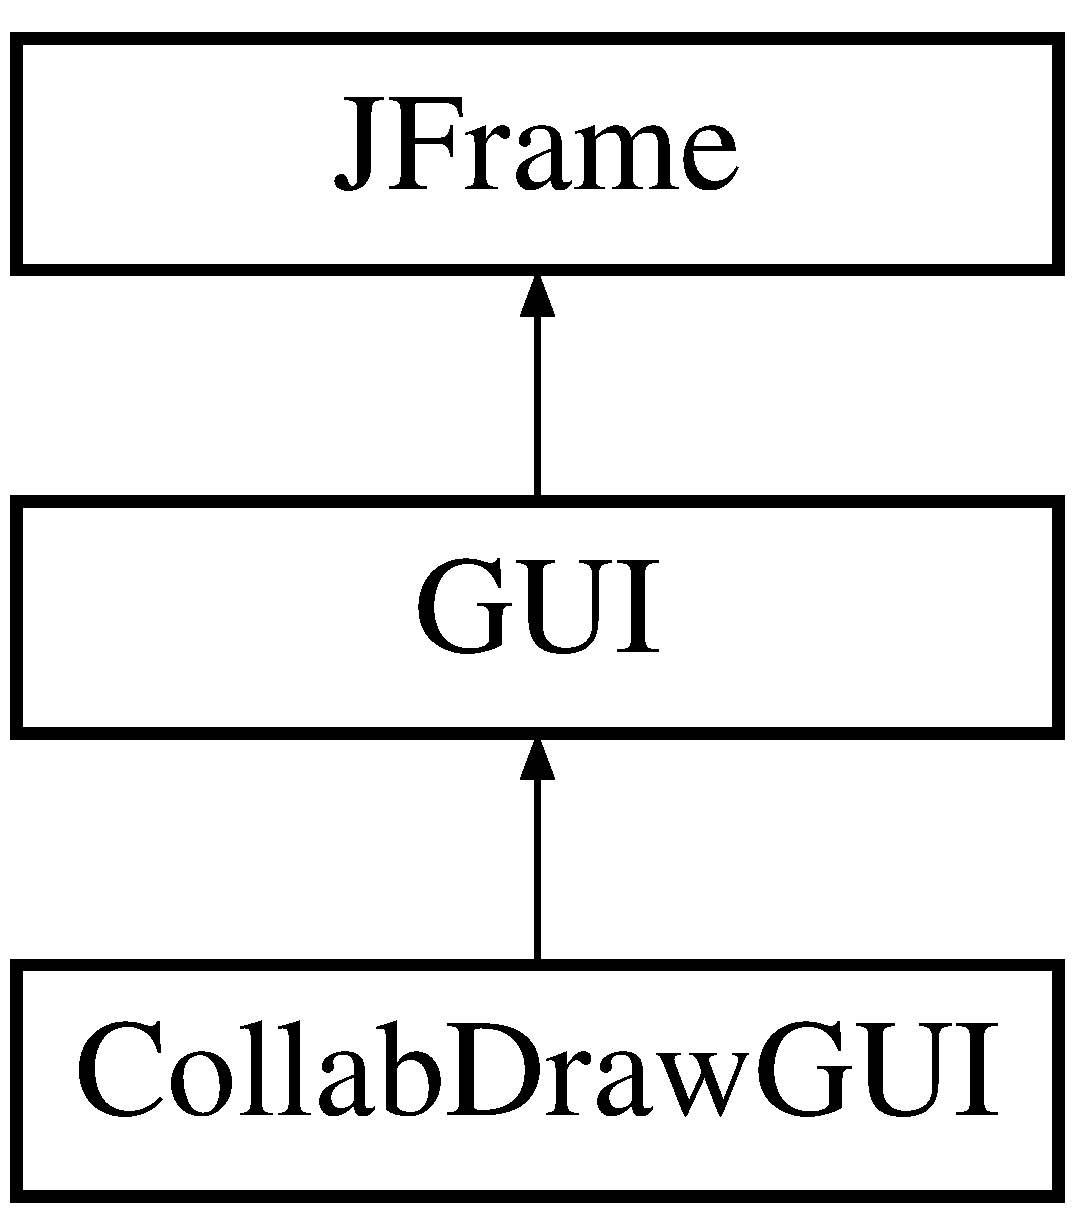
\includegraphics[height=3.000000cm]{class_collab_draw_g_u_i}
\end{center}
\end{figure}
\subsection*{Public Member Functions}
\begin{DoxyCompactItemize}
\item 
\mbox{\Hypertarget{class_collab_draw_g_u_i_ac8f9c49ca65d4c8a85406c4c0e2f638a}\label{class_collab_draw_g_u_i_ac8f9c49ca65d4c8a85406c4c0e2f638a}} 
\hyperlink{class_collab_draw_g_u_i_ac8f9c49ca65d4c8a85406c4c0e2f638a}{Collab\+Draw\+G\+UI} (\hyperlink{class_account}{Account} a1, \hyperlink{class_account}{Account} a2)  throws Exception 
\begin{DoxyCompactList}\small\item\em Constructor\+: inherits methods and attributes from \hyperlink{class_g_u_i}{G\+UI} and loads elements onto window through load\+Elements(). \end{DoxyCompactList}\end{DoxyCompactItemize}
\subsection*{Static Public Member Functions}
\begin{DoxyCompactItemize}
\item 
\mbox{\Hypertarget{class_collab_draw_g_u_i_a0339e463a885aed96a0fb5d976d6fef3}\label{class_collab_draw_g_u_i_a0339e463a885aed96a0fb5d976d6fef3}} 
static void {\bfseries main} (String\mbox{[}$\,$\mbox{]} args)  throws Exception 
\end{DoxyCompactItemize}


The documentation for this class was generated from the following file\+:\begin{DoxyCompactItemize}
\item 
readwrite/Collab\+Draw\+G\+U\+I.\+java\end{DoxyCompactItemize}

\hypertarget{class_create_account_g_u_i}{}\section{Create\+Account\+G\+UI Class Reference}
\label{class_create_account_g_u_i}\index{Create\+Account\+G\+UI@{Create\+Account\+G\+UI}}
Inheritance diagram for Create\+Account\+G\+UI\+:\begin{figure}[H]
\begin{center}
\leavevmode
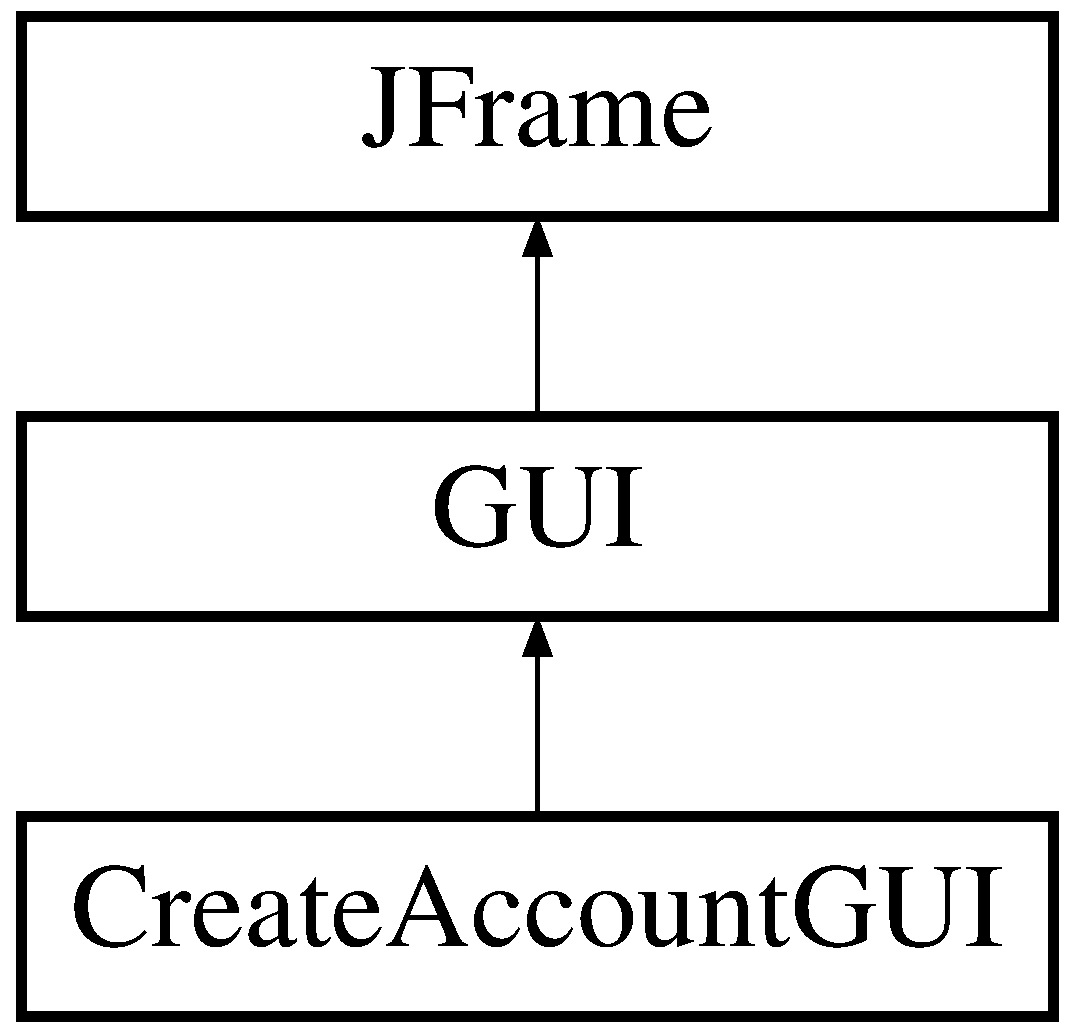
\includegraphics[height=3.000000cm]{class_create_account_g_u_i}
\end{center}
\end{figure}
\subsection*{Public Member Functions}
\begin{DoxyCompactItemize}
\item 
\mbox{\Hypertarget{class_create_account_g_u_i_aad1fa44b4ad6345b06a03e8f4cc10f17}\label{class_create_account_g_u_i_aad1fa44b4ad6345b06a03e8f4cc10f17}} 
\hyperlink{class_create_account_g_u_i_aad1fa44b4ad6345b06a03e8f4cc10f17}{Create\+Account\+G\+UI} ()  throws Exception
\begin{DoxyCompactList}\small\item\em Builds a form the user can input to and generates an \hyperlink{class_account}{Account} object that is written directly to the db. \end{DoxyCompactList}\end{DoxyCompactItemize}
\subsection*{Static Public Member Functions}
\begin{DoxyCompactItemize}
\item 
\mbox{\Hypertarget{class_create_account_g_u_i_ac8094edda569c99d4d88f9d27fe64e24}\label{class_create_account_g_u_i_ac8094edda569c99d4d88f9d27fe64e24}} 
static void \hyperlink{class_create_account_g_u_i_ac8094edda569c99d4d88f9d27fe64e24}{make\+Form} (Container parent, int rows, int cols, int initialX, int initialY, int x\+Pad, int y\+Pad)  throws Exception 
\begin{DoxyCompactList}\small\item\em Generates the forms layout. \end{DoxyCompactList}\item 
\mbox{\Hypertarget{class_create_account_g_u_i_a4ef58270bb46ae0431a317cfe5efb162}\label{class_create_account_g_u_i_a4ef58270bb46ae0431a317cfe5efb162}} 
static void \hyperlink{class_create_account_g_u_i_a4ef58270bb46ae0431a317cfe5efb162}{main} (String\mbox{[}$\,$\mbox{]} args)  throws Exception 
\begin{DoxyCompactList}\small\item\em Implemented for testing purposes. \end{DoxyCompactList}\end{DoxyCompactItemize}


The documentation for this class was generated from the following file\+:\begin{DoxyCompactItemize}
\item 
readwrite/Create\+Account\+G\+U\+I.\+java\end{DoxyCompactItemize}

\hypertarget{class_drawing_panel}{}\section{Drawing\+Panel Class Reference}
\label{class_drawing_panel}\index{Drawing\+Panel@{Drawing\+Panel}}
Inheritance diagram for Drawing\+Panel\+:\begin{figure}[H]
\begin{center}
\leavevmode
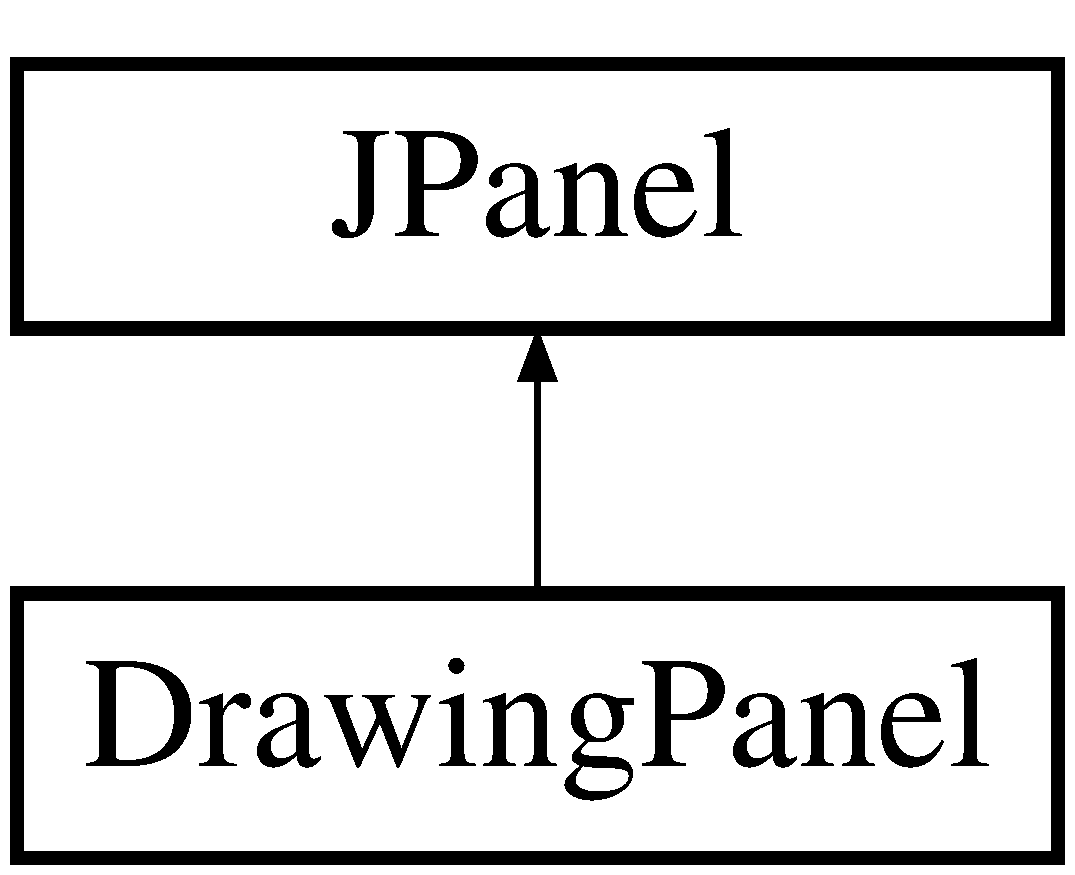
\includegraphics[height=2.000000cm]{class_drawing_panel}
\end{center}
\end{figure}
\subsection*{Public Member Functions}
\begin{DoxyCompactItemize}
\item 
Array\+List$<$ \hyperlink{class_line}{Line} $>$ \hyperlink{class_drawing_panel_a3f8dc5d1f652dd58859ca98dce3e325b}{get\+Lines} ()
\begin{DoxyCompactList}\small\item\em Method to return the Array\+List of lines drawn to screen. \end{DoxyCompactList}\item 
int \hyperlink{class_drawing_panel_a77c3fd72e4c60f65d043ff01e7a8802d}{get\+Point\+Count} ()
\begin{DoxyCompactList}\small\item\em Method to retrieve number of points drawn on screen. \end{DoxyCompactList}\item 
boolean \hyperlink{class_drawing_panel_a4b121aedcf7c0c4a333519db1e340a9b}{increment\+Point\+Count} ()
\begin{DoxyCompactList}\small\item\em Increments the point count. \end{DoxyCompactList}\item 
Point \mbox{[}$\,$\mbox{]} \hyperlink{class_drawing_panel_a7622f1394438b6ec633ac2cde884bb99}{get\+Points} ()
\begin{DoxyCompactList}\small\item\em Returns the array of points drawn on screen. \end{DoxyCompactList}\item 
Color \hyperlink{class_drawing_panel_ae0c2b7deb6ba8eae624e58c850a3a559}{get\+Drawn\+Colour} ()
\begin{DoxyCompactList}\small\item\em Method to retrieve the colour of a drawing. \end{DoxyCompactList}\item 
Color \mbox{[}$\,$\mbox{]} \hyperlink{class_drawing_panel_a90f962e27cca561096b4d5a68fd69ac3}{get\+Colours} ()
\begin{DoxyCompactList}\small\item\em Method to retrieve the array of colours in a trace. \end{DoxyCompactList}\item 
boolean \hyperlink{class_drawing_panel_a7eae2c9bc64af0b4bcb177370598b3ad}{set\+Trace\+Point} (Point point)
\begin{DoxyCompactList}\small\item\em Method to set the point of trace at current point count in array. \end{DoxyCompactList}\item 
void \hyperlink{class_drawing_panel_a7fdcb0fc4a40945930517bdf664d6179}{set\+Draw\+Tool} (String draw\+Tool)
\begin{DoxyCompactList}\small\item\em Method to allow user to switch between line and particle trace. \end{DoxyCompactList}\item 
void \hyperlink{class_drawing_panel_a9e295a2f6aec0c5e85240324dff07d90}{set\+Point\+Color} (Color colour)
\begin{DoxyCompactList}\small\item\em Method to set the colour of a point in a particle trace. \end{DoxyCompactList}\item 
void \hyperlink{class_drawing_panel_a7b1a3aaefb7f62604525ebb494f6faa6}{set\+Draw\+Colour} (Color colour)
\begin{DoxyCompactList}\small\item\em Method to set the colour of a drawing. \end{DoxyCompactList}\item 
void \hyperlink{class_drawing_panel_a4efd38d997c0ddf31cc49ca18898484d}{set\+Line\+Begin} (Point point)
\begin{DoxyCompactList}\small\item\em Method to set the point at the start of a drawn line. \end{DoxyCompactList}\item 
void \hyperlink{class_drawing_panel_abf64c73a6dced3ea8183a2354a06cae7}{set\+Line\+Finish} (Point point)
\begin{DoxyCompactList}\small\item\em Method to set the point at the end of a drawn line. \end{DoxyCompactList}\item 
void \hyperlink{class_drawing_panel_abf082fafa7877579ae1bf1583e74cdd8}{add\+Lines} (\hyperlink{class_line}{Line} line)
\begin{DoxyCompactList}\small\item\em Method to add drawn lines to the line Array\+List. \end{DoxyCompactList}\item 
void \hyperlink{class_drawing_panel_a7fd34e1524b98d70607998bafbc71d8b}{set\+Array\+List\+Lines} (Array\+List$<$ \hyperlink{class_line}{Line} $>$ line)
\begin{DoxyCompactList}\small\item\em Method to set the Array\+List of lines. \end{DoxyCompactList}\item 
void \hyperlink{class_drawing_panel_a47cd7b7965dd2cb7e63f56a2737ffe39}{set\+All\+Trace\+Points} (Point\mbox{[}$\,$\mbox{]} point)
\begin{DoxyCompactList}\small\item\em Method to set the array of drawn points in a particle trace. \end{DoxyCompactList}\item 
void \hyperlink{class_drawing_panel_a3c4886846e221ed78b1859d0d022cf8f}{set\+Point\+Count} (int count)
\begin{DoxyCompactList}\small\item\em Method to set the count of points drawn. \end{DoxyCompactList}\item 
void \hyperlink{class_drawing_panel_a9816f7a7b7aeefeb6f0e5d9321eb94a2}{set\+All\+Point\+Color} (Color\mbox{[}$\,$\mbox{]} array\+Of\+Colours)
\begin{DoxyCompactList}\small\item\em Method to set the colours of all points draw in a trace draw. \end{DoxyCompactList}\item 
\hyperlink{class_drawing_panel_a63d04db10fba53e2b46d536525d278ac}{Drawing\+Panel} (\hyperlink{class_account}{Account} sender, \hyperlink{class_account}{Account} recipient)
\begin{DoxyCompactList}\small\item\em T\+O\+DO \+: C\+O\+M\+P\+A\+R\+I\+NG T\+HE A\+C\+C\+O\+U\+N\+TS U\+S\+E\+R\+N\+A\+M\+ES TO M\+A\+KE A T\+E\+XT F\+I\+LE W\+I\+TH T\+HE T\+WO U\+S\+E\+R\+N\+A\+M\+ES AS T\+HE T\+E\+XT F\+I\+LE\textquotesingle{}S N\+A\+ME. \end{DoxyCompactList}\item 
void \hyperlink{class_drawing_panel_a9fe458b4cbb53b245a7d7edc0a2d1e83}{save\+Line} (Array\+List$<$ \hyperlink{class_line}{Line} $>$ drawn\+Line)  throws I\+O\+Exception 
\begin{DoxyCompactList}\small\item\em Method to save the drawn line to the line file. \end{DoxyCompactList}\item 
void \hyperlink{class_drawing_panel_a3c4bdf70ae72b099b258040244f9d428}{save\+Partical} (Point\mbox{[}$\,$\mbox{]} trace, Color\mbox{[}$\,$\mbox{]} trace\+Colour)  throws I\+O\+Exception 
\begin{DoxyCompactList}\small\item\em Method to save all particle trace drawings. \end{DoxyCompactList}\item 
void \hyperlink{class_drawing_panel_a94f31c4cf6856ae742da17f00d8b33e4}{paint\+Component} (Graphics g)
\begin{DoxyCompactList}\small\item\em Draw an oval in a O\+V\+A\+L\+\_\+\+W\+I\+D\+T\+H-\/by-\/\+O\+V\+A\+L\+\_\+\+H\+E\+I\+G\+HT bounding box at specified x and y in a specified colour on window. \end{DoxyCompactList}\item 
void \hyperlink{class_drawing_panel_a72ba678075cd06d0455dddfe2509da83}{load\+Line\+File} (String line\+File)
\begin{DoxyCompactList}\small\item\em Method to load a line file, parse through its contents and repaint on screen. \end{DoxyCompactList}\item 
void \hyperlink{class_drawing_panel_a2c3c19d065415dfffacfb2ded1fb114a}{load\+Particle\+File} (String particle\+Trace\+File)
\begin{DoxyCompactList}\small\item\em Method to load a particle trace file, parse through its contents and repaint on screen. \end{DoxyCompactList}\end{DoxyCompactItemize}


\subsection{Constructor \& Destructor Documentation}
\mbox{\Hypertarget{class_drawing_panel_a63d04db10fba53e2b46d536525d278ac}\label{class_drawing_panel_a63d04db10fba53e2b46d536525d278ac}} 
\index{Drawing\+Panel@{Drawing\+Panel}!Drawing\+Panel@{Drawing\+Panel}}
\index{Drawing\+Panel@{Drawing\+Panel}!Drawing\+Panel@{Drawing\+Panel}}
\subsubsection{\texorpdfstring{Drawing\+Panel()}{DrawingPanel()}}
{\footnotesize\ttfamily Drawing\+Panel.\+Drawing\+Panel (\begin{DoxyParamCaption}\item[{\hyperlink{class_account}{Account}}]{sender,  }\item[{\hyperlink{class_account}{Account}}]{recipient }\end{DoxyParamCaption})}



T\+O\+DO \+: C\+O\+M\+P\+A\+R\+I\+NG T\+HE A\+C\+C\+O\+U\+N\+TS U\+S\+E\+R\+N\+A\+M\+ES TO M\+A\+KE A T\+E\+XT F\+I\+LE W\+I\+TH T\+HE T\+WO U\+S\+E\+R\+N\+A\+M\+ES AS T\+HE T\+E\+XT F\+I\+LE\textquotesingle{}S N\+A\+ME. 

Constructor\+: set up \hyperlink{class_g_u_i}{G\+UI} by loading the file amd repainting on screen. T\+HE C\+O\+N\+S\+T\+R\+U\+C\+T\+OR A\+L\+W\+A\+YS L\+O\+A\+DS A T\+E\+XT F\+I\+LE W\+H\+EN I\+TS C\+A\+L\+L\+ED, SO M\+A\+Y\+BE WE C\+O\+U\+LD C\+R\+E\+A\+TE AN E\+M\+P\+TY T\+E\+XT F\+I\+LE W\+H\+EN A F\+R\+I\+E\+N\+D\+S\+H\+IP IS C\+R\+E\+A\+T\+ED, SO T\+H\+AT A T\+E\+XT F\+I\+LE W\+I\+LL A\+L\+W\+A\+YS BE F\+O\+U\+ND?

\subsection{Member Function Documentation}
\mbox{\Hypertarget{class_drawing_panel_abf082fafa7877579ae1bf1583e74cdd8}\label{class_drawing_panel_abf082fafa7877579ae1bf1583e74cdd8}} 
\index{Drawing\+Panel@{Drawing\+Panel}!add\+Lines@{add\+Lines}}
\index{add\+Lines@{add\+Lines}!Drawing\+Panel@{Drawing\+Panel}}
\subsubsection{\texorpdfstring{add\+Lines()}{addLines()}}
{\footnotesize\ttfamily void Drawing\+Panel.\+add\+Lines (\begin{DoxyParamCaption}\item[{\hyperlink{class_line}{Line}}]{line }\end{DoxyParamCaption})}



Method to add drawn lines to the line Array\+List. 


\begin{DoxyParams}{Parameters}
{\em \hyperlink{class_line}{Line}} & to be added to the Array\+List. \\
\hline
\end{DoxyParams}
\mbox{\Hypertarget{class_drawing_panel_a90f962e27cca561096b4d5a68fd69ac3}\label{class_drawing_panel_a90f962e27cca561096b4d5a68fd69ac3}} 
\index{Drawing\+Panel@{Drawing\+Panel}!get\+Colours@{get\+Colours}}
\index{get\+Colours@{get\+Colours}!Drawing\+Panel@{Drawing\+Panel}}
\subsubsection{\texorpdfstring{get\+Colours()}{getColours()}}
{\footnotesize\ttfamily Color \mbox{[}$\,$\mbox{]} Drawing\+Panel.\+get\+Colours (\begin{DoxyParamCaption}{ }\end{DoxyParamCaption})}



Method to retrieve the array of colours in a trace. 

\begin{DoxyReturn}{Returns}
the array of colour of the point in trace. 
\end{DoxyReturn}
\mbox{\Hypertarget{class_drawing_panel_ae0c2b7deb6ba8eae624e58c850a3a559}\label{class_drawing_panel_ae0c2b7deb6ba8eae624e58c850a3a559}} 
\index{Drawing\+Panel@{Drawing\+Panel}!get\+Drawn\+Colour@{get\+Drawn\+Colour}}
\index{get\+Drawn\+Colour@{get\+Drawn\+Colour}!Drawing\+Panel@{Drawing\+Panel}}
\subsubsection{\texorpdfstring{get\+Drawn\+Colour()}{getDrawnColour()}}
{\footnotesize\ttfamily Color Drawing\+Panel.\+get\+Drawn\+Colour (\begin{DoxyParamCaption}{ }\end{DoxyParamCaption})}



Method to retrieve the colour of a drawing. 

\begin{DoxyReturn}{Returns}
the current colour of drawing 
\end{DoxyReturn}
\mbox{\Hypertarget{class_drawing_panel_a3f8dc5d1f652dd58859ca98dce3e325b}\label{class_drawing_panel_a3f8dc5d1f652dd58859ca98dce3e325b}} 
\index{Drawing\+Panel@{Drawing\+Panel}!get\+Lines@{get\+Lines}}
\index{get\+Lines@{get\+Lines}!Drawing\+Panel@{Drawing\+Panel}}
\subsubsection{\texorpdfstring{get\+Lines()}{getLines()}}
{\footnotesize\ttfamily Array\+List$<$\hyperlink{class_line}{Line}$>$ Drawing\+Panel.\+get\+Lines (\begin{DoxyParamCaption}{ }\end{DoxyParamCaption})}



Method to return the Array\+List of lines drawn to screen. 

\begin{DoxyReturn}{Returns}
the Array\+List of lines. 
\end{DoxyReturn}
\mbox{\Hypertarget{class_drawing_panel_a77c3fd72e4c60f65d043ff01e7a8802d}\label{class_drawing_panel_a77c3fd72e4c60f65d043ff01e7a8802d}} 
\index{Drawing\+Panel@{Drawing\+Panel}!get\+Point\+Count@{get\+Point\+Count}}
\index{get\+Point\+Count@{get\+Point\+Count}!Drawing\+Panel@{Drawing\+Panel}}
\subsubsection{\texorpdfstring{get\+Point\+Count()}{getPointCount()}}
{\footnotesize\ttfamily int Drawing\+Panel.\+get\+Point\+Count (\begin{DoxyParamCaption}{ }\end{DoxyParamCaption})}



Method to retrieve number of points drawn on screen. 

\begin{DoxyReturn}{Returns}
the number of points 
\end{DoxyReturn}
\mbox{\Hypertarget{class_drawing_panel_a7622f1394438b6ec633ac2cde884bb99}\label{class_drawing_panel_a7622f1394438b6ec633ac2cde884bb99}} 
\index{Drawing\+Panel@{Drawing\+Panel}!get\+Points@{get\+Points}}
\index{get\+Points@{get\+Points}!Drawing\+Panel@{Drawing\+Panel}}
\subsubsection{\texorpdfstring{get\+Points()}{getPoints()}}
{\footnotesize\ttfamily Point \mbox{[}$\,$\mbox{]} Drawing\+Panel.\+get\+Points (\begin{DoxyParamCaption}{ }\end{DoxyParamCaption})}



Returns the array of points drawn on screen. 

\begin{DoxyReturn}{Returns}
the current number of points 
\end{DoxyReturn}
\mbox{\Hypertarget{class_drawing_panel_a4b121aedcf7c0c4a333519db1e340a9b}\label{class_drawing_panel_a4b121aedcf7c0c4a333519db1e340a9b}} 
\index{Drawing\+Panel@{Drawing\+Panel}!increment\+Point\+Count@{increment\+Point\+Count}}
\index{increment\+Point\+Count@{increment\+Point\+Count}!Drawing\+Panel@{Drawing\+Panel}}
\subsubsection{\texorpdfstring{increment\+Point\+Count()}{incrementPointCount()}}
{\footnotesize\ttfamily boolean Drawing\+Panel.\+increment\+Point\+Count (\begin{DoxyParamCaption}{ }\end{DoxyParamCaption})}



Increments the point count. 

\begin{DoxyReturn}{Returns}
T\+R\+UE on success 
\end{DoxyReturn}
\mbox{\Hypertarget{class_drawing_panel_a72ba678075cd06d0455dddfe2509da83}\label{class_drawing_panel_a72ba678075cd06d0455dddfe2509da83}} 
\index{Drawing\+Panel@{Drawing\+Panel}!load\+Line\+File@{load\+Line\+File}}
\index{load\+Line\+File@{load\+Line\+File}!Drawing\+Panel@{Drawing\+Panel}}
\subsubsection{\texorpdfstring{load\+Line\+File()}{loadLineFile()}}
{\footnotesize\ttfamily void Drawing\+Panel.\+load\+Line\+File (\begin{DoxyParamCaption}\item[{String}]{line\+File }\end{DoxyParamCaption})}



Method to load a line file, parse through its contents and repaint on screen. 


\begin{DoxyParams}{Parameters}
{\em the} & filename of the line file. \\
\hline
\end{DoxyParams}
\mbox{\Hypertarget{class_drawing_panel_a2c3c19d065415dfffacfb2ded1fb114a}\label{class_drawing_panel_a2c3c19d065415dfffacfb2ded1fb114a}} 
\index{Drawing\+Panel@{Drawing\+Panel}!load\+Particle\+File@{load\+Particle\+File}}
\index{load\+Particle\+File@{load\+Particle\+File}!Drawing\+Panel@{Drawing\+Panel}}
\subsubsection{\texorpdfstring{load\+Particle\+File()}{loadParticleFile()}}
{\footnotesize\ttfamily void Drawing\+Panel.\+load\+Particle\+File (\begin{DoxyParamCaption}\item[{String}]{particle\+Trace\+File }\end{DoxyParamCaption})}



Method to load a particle trace file, parse through its contents and repaint on screen. 


\begin{DoxyParams}{Parameters}
{\em the} & filename of the particle trace file. \\
\hline
\end{DoxyParams}
\mbox{\Hypertarget{class_drawing_panel_a94f31c4cf6856ae742da17f00d8b33e4}\label{class_drawing_panel_a94f31c4cf6856ae742da17f00d8b33e4}} 
\index{Drawing\+Panel@{Drawing\+Panel}!paint\+Component@{paint\+Component}}
\index{paint\+Component@{paint\+Component}!Drawing\+Panel@{Drawing\+Panel}}
\subsubsection{\texorpdfstring{paint\+Component()}{paintComponent()}}
{\footnotesize\ttfamily void Drawing\+Panel.\+paint\+Component (\begin{DoxyParamCaption}\item[{Graphics}]{g }\end{DoxyParamCaption})}



Draw an oval in a O\+V\+A\+L\+\_\+\+W\+I\+D\+T\+H-\/by-\/\+O\+V\+A\+L\+\_\+\+H\+E\+I\+G\+HT bounding box at specified x and y in a specified colour on window. 

This method is called from Paint\+Handler\+::mouse\+Dragged().

Draws a line between starting x,y and ending x,y in the specified colour on window. This is called from Paint\+Handler\+::mouse\+Released(). \mbox{\Hypertarget{class_drawing_panel_a9fe458b4cbb53b245a7d7edc0a2d1e83}\label{class_drawing_panel_a9fe458b4cbb53b245a7d7edc0a2d1e83}} 
\index{Drawing\+Panel@{Drawing\+Panel}!save\+Line@{save\+Line}}
\index{save\+Line@{save\+Line}!Drawing\+Panel@{Drawing\+Panel}}
\subsubsection{\texorpdfstring{save\+Line()}{saveLine()}}
{\footnotesize\ttfamily void Drawing\+Panel.\+save\+Line (\begin{DoxyParamCaption}\item[{Array\+List$<$ \hyperlink{class_line}{Line} $>$}]{drawn\+Line }\end{DoxyParamCaption}) throws I\+O\+Exception}



Method to save the drawn line to the line file. 

This throws an I\+O\+Exception. 
\begin{DoxyParams}{Parameters}
{\em Array\+List} & of drawn lines from the window. \\
\hline
\end{DoxyParams}
\mbox{\Hypertarget{class_drawing_panel_a3c4bdf70ae72b099b258040244f9d428}\label{class_drawing_panel_a3c4bdf70ae72b099b258040244f9d428}} 
\index{Drawing\+Panel@{Drawing\+Panel}!save\+Partical@{save\+Partical}}
\index{save\+Partical@{save\+Partical}!Drawing\+Panel@{Drawing\+Panel}}
\subsubsection{\texorpdfstring{save\+Partical()}{savePartical()}}
{\footnotesize\ttfamily void Drawing\+Panel.\+save\+Partical (\begin{DoxyParamCaption}\item[{Point \mbox{[}$\,$\mbox{]}}]{trace,  }\item[{Color \mbox{[}$\,$\mbox{]}}]{trace\+Colour }\end{DoxyParamCaption}) throws I\+O\+Exception}



Method to save all particle trace drawings. 

This throws an I\+O\+Exception. 
\begin{DoxyParams}{Parameters}
{\em array} & of drawn points on screen. \\
\hline
{\em array} & of colours of these drawn points. \\
\hline
\end{DoxyParams}
\mbox{\Hypertarget{class_drawing_panel_a9816f7a7b7aeefeb6f0e5d9321eb94a2}\label{class_drawing_panel_a9816f7a7b7aeefeb6f0e5d9321eb94a2}} 
\index{Drawing\+Panel@{Drawing\+Panel}!set\+All\+Point\+Color@{set\+All\+Point\+Color}}
\index{set\+All\+Point\+Color@{set\+All\+Point\+Color}!Drawing\+Panel@{Drawing\+Panel}}
\subsubsection{\texorpdfstring{set\+All\+Point\+Color()}{setAllPointColor()}}
{\footnotesize\ttfamily void Drawing\+Panel.\+set\+All\+Point\+Color (\begin{DoxyParamCaption}\item[{Color \mbox{[}$\,$\mbox{]}}]{array\+Of\+Colours }\end{DoxyParamCaption})}



Method to set the colours of all points draw in a trace draw. 


\begin{DoxyParams}{Parameters}
{\em the} & array of colours. \\
\hline
\end{DoxyParams}
\mbox{\Hypertarget{class_drawing_panel_a47cd7b7965dd2cb7e63f56a2737ffe39}\label{class_drawing_panel_a47cd7b7965dd2cb7e63f56a2737ffe39}} 
\index{Drawing\+Panel@{Drawing\+Panel}!set\+All\+Trace\+Points@{set\+All\+Trace\+Points}}
\index{set\+All\+Trace\+Points@{set\+All\+Trace\+Points}!Drawing\+Panel@{Drawing\+Panel}}
\subsubsection{\texorpdfstring{set\+All\+Trace\+Points()}{setAllTracePoints()}}
{\footnotesize\ttfamily void Drawing\+Panel.\+set\+All\+Trace\+Points (\begin{DoxyParamCaption}\item[{Point \mbox{[}$\,$\mbox{]}}]{point }\end{DoxyParamCaption})}



Method to set the array of drawn points in a particle trace. 


\begin{DoxyParams}{Parameters}
{\em the} & array of points. \\
\hline
\end{DoxyParams}
\mbox{\Hypertarget{class_drawing_panel_a7fd34e1524b98d70607998bafbc71d8b}\label{class_drawing_panel_a7fd34e1524b98d70607998bafbc71d8b}} 
\index{Drawing\+Panel@{Drawing\+Panel}!set\+Array\+List\+Lines@{set\+Array\+List\+Lines}}
\index{set\+Array\+List\+Lines@{set\+Array\+List\+Lines}!Drawing\+Panel@{Drawing\+Panel}}
\subsubsection{\texorpdfstring{set\+Array\+List\+Lines()}{setArrayListLines()}}
{\footnotesize\ttfamily void Drawing\+Panel.\+set\+Array\+List\+Lines (\begin{DoxyParamCaption}\item[{Array\+List$<$ \hyperlink{class_line}{Line} $>$}]{line }\end{DoxyParamCaption})}



Method to set the Array\+List of lines. 


\begin{DoxyParams}{Parameters}
{\em the} & Array\+List of lines. \\
\hline
\end{DoxyParams}
\mbox{\Hypertarget{class_drawing_panel_a7b1a3aaefb7f62604525ebb494f6faa6}\label{class_drawing_panel_a7b1a3aaefb7f62604525ebb494f6faa6}} 
\index{Drawing\+Panel@{Drawing\+Panel}!set\+Draw\+Colour@{set\+Draw\+Colour}}
\index{set\+Draw\+Colour@{set\+Draw\+Colour}!Drawing\+Panel@{Drawing\+Panel}}
\subsubsection{\texorpdfstring{set\+Draw\+Colour()}{setDrawColour()}}
{\footnotesize\ttfamily void Drawing\+Panel.\+set\+Draw\+Colour (\begin{DoxyParamCaption}\item[{Color}]{colour }\end{DoxyParamCaption})}



Method to set the colour of a drawing. 


\begin{DoxyParams}{Parameters}
{\em the} & colour to be set. \\
\hline
\end{DoxyParams}
\mbox{\Hypertarget{class_drawing_panel_a7fdcb0fc4a40945930517bdf664d6179}\label{class_drawing_panel_a7fdcb0fc4a40945930517bdf664d6179}} 
\index{Drawing\+Panel@{Drawing\+Panel}!set\+Draw\+Tool@{set\+Draw\+Tool}}
\index{set\+Draw\+Tool@{set\+Draw\+Tool}!Drawing\+Panel@{Drawing\+Panel}}
\subsubsection{\texorpdfstring{set\+Draw\+Tool()}{setDrawTool()}}
{\footnotesize\ttfamily void Drawing\+Panel.\+set\+Draw\+Tool (\begin{DoxyParamCaption}\item[{String}]{draw\+Tool }\end{DoxyParamCaption})}



Method to allow user to switch between line and particle trace. 


\begin{DoxyParams}{Parameters}
{\em mode} & \\
\hline
\end{DoxyParams}
\mbox{\Hypertarget{class_drawing_panel_a4efd38d997c0ddf31cc49ca18898484d}\label{class_drawing_panel_a4efd38d997c0ddf31cc49ca18898484d}} 
\index{Drawing\+Panel@{Drawing\+Panel}!set\+Line\+Begin@{set\+Line\+Begin}}
\index{set\+Line\+Begin@{set\+Line\+Begin}!Drawing\+Panel@{Drawing\+Panel}}
\subsubsection{\texorpdfstring{set\+Line\+Begin()}{setLineBegin()}}
{\footnotesize\ttfamily void Drawing\+Panel.\+set\+Line\+Begin (\begin{DoxyParamCaption}\item[{Point}]{point }\end{DoxyParamCaption})}



Method to set the point at the start of a drawn line. 


\begin{DoxyParams}{Parameters}
{\em the} & point at the start of the line. \\
\hline
\end{DoxyParams}
\mbox{\Hypertarget{class_drawing_panel_abf64c73a6dced3ea8183a2354a06cae7}\label{class_drawing_panel_abf64c73a6dced3ea8183a2354a06cae7}} 
\index{Drawing\+Panel@{Drawing\+Panel}!set\+Line\+Finish@{set\+Line\+Finish}}
\index{set\+Line\+Finish@{set\+Line\+Finish}!Drawing\+Panel@{Drawing\+Panel}}
\subsubsection{\texorpdfstring{set\+Line\+Finish()}{setLineFinish()}}
{\footnotesize\ttfamily void Drawing\+Panel.\+set\+Line\+Finish (\begin{DoxyParamCaption}\item[{Point}]{point }\end{DoxyParamCaption})}



Method to set the point at the end of a drawn line. 


\begin{DoxyParams}{Parameters}
{\em the} & point at the start of the line. \\
\hline
\end{DoxyParams}
\mbox{\Hypertarget{class_drawing_panel_a9e295a2f6aec0c5e85240324dff07d90}\label{class_drawing_panel_a9e295a2f6aec0c5e85240324dff07d90}} 
\index{Drawing\+Panel@{Drawing\+Panel}!set\+Point\+Color@{set\+Point\+Color}}
\index{set\+Point\+Color@{set\+Point\+Color}!Drawing\+Panel@{Drawing\+Panel}}
\subsubsection{\texorpdfstring{set\+Point\+Color()}{setPointColor()}}
{\footnotesize\ttfamily void Drawing\+Panel.\+set\+Point\+Color (\begin{DoxyParamCaption}\item[{Color}]{colour }\end{DoxyParamCaption})}



Method to set the colour of a point in a particle trace. 


\begin{DoxyParams}{Parameters}
{\em the} & colour to be set at a certain point. \\
\hline
\end{DoxyParams}
\mbox{\Hypertarget{class_drawing_panel_a3c4886846e221ed78b1859d0d022cf8f}\label{class_drawing_panel_a3c4886846e221ed78b1859d0d022cf8f}} 
\index{Drawing\+Panel@{Drawing\+Panel}!set\+Point\+Count@{set\+Point\+Count}}
\index{set\+Point\+Count@{set\+Point\+Count}!Drawing\+Panel@{Drawing\+Panel}}
\subsubsection{\texorpdfstring{set\+Point\+Count()}{setPointCount()}}
{\footnotesize\ttfamily void Drawing\+Panel.\+set\+Point\+Count (\begin{DoxyParamCaption}\item[{int}]{count }\end{DoxyParamCaption})}



Method to set the count of points drawn. 


\begin{DoxyParams}{Parameters}
{\em the} & count of drawn points. \\
\hline
\end{DoxyParams}
\mbox{\Hypertarget{class_drawing_panel_a7eae2c9bc64af0b4bcb177370598b3ad}\label{class_drawing_panel_a7eae2c9bc64af0b4bcb177370598b3ad}} 
\index{Drawing\+Panel@{Drawing\+Panel}!set\+Trace\+Point@{set\+Trace\+Point}}
\index{set\+Trace\+Point@{set\+Trace\+Point}!Drawing\+Panel@{Drawing\+Panel}}
\subsubsection{\texorpdfstring{set\+Trace\+Point()}{setTracePoint()}}
{\footnotesize\ttfamily boolean Drawing\+Panel.\+set\+Trace\+Point (\begin{DoxyParamCaption}\item[{Point}]{point }\end{DoxyParamCaption})}



Method to set the point of trace at current point count in array. 


\begin{DoxyParams}{Parameters}
{\em point} & \\
\hline
\end{DoxyParams}
\begin{DoxyReturn}{Returns}
T\+R\+UE on success 
\end{DoxyReturn}


The documentation for this class was generated from the following file\+:\begin{DoxyCompactItemize}
\item 
readwrite/Drawing\+Panel.\+java\end{DoxyCompactItemize}

\hypertarget{class_edge}{}\section{Edge Class Reference}
\label{class_edge}\index{Edge@{Edge}}


The \hyperlink{class_edge}{Edge} class is used in the \hyperlink{class_graph}{Graph} and \hyperlink{class_vertex}{Vertex} classes.  


Inheritance diagram for Edge\+:\begin{figure}[H]
\begin{center}
\leavevmode
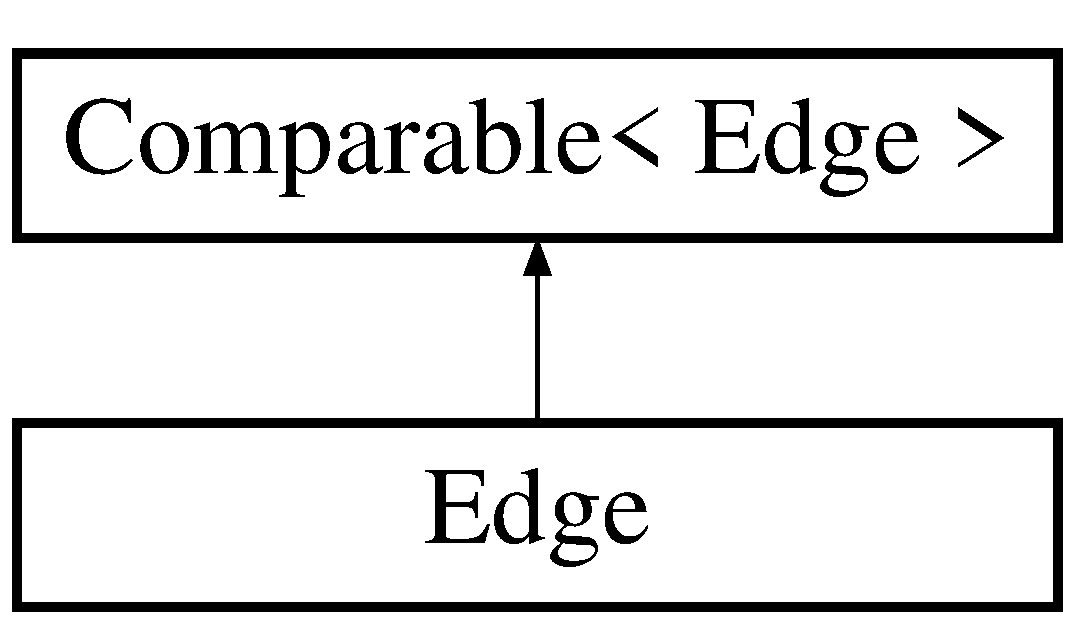
\includegraphics[height=2.000000cm]{class_edge}
\end{center}
\end{figure}
\subsection*{Public Member Functions}
\begin{DoxyCompactItemize}
\item 
\hyperlink{class_edge_ad763d55acaac9dea971255819e8fde06}{Edge} (\hyperlink{class_vertex}{Vertex} one, \hyperlink{class_vertex}{Vertex} two)
\begin{DoxyCompactList}\small\item\em constructor for edge \end{DoxyCompactList}\item 
\hyperlink{class_edge_a5b282bda21b36ca17d9c3614943d5387}{Edge} (\hyperlink{class_vertex}{Vertex} one, \hyperlink{class_vertex}{Vertex} two, int weight)
\begin{DoxyCompactList}\small\item\em alternative constructor for edge \end{DoxyCompactList}\item 
\hyperlink{class_vertex}{Vertex} \hyperlink{class_edge_abf42bcb6e0c33e5a66e73170d4591522}{get\+Vertices} (\hyperlink{class_vertex}{Vertex} current)
\begin{DoxyCompactList}\small\item\em return the neighbour vertex along this edge \end{DoxyCompactList}\item 
\hyperlink{class_vertex}{Vertex} \hyperlink{class_edge_ab980e6d28be975d55e1ccffaffd173fd}{get\+One} ()
\begin{DoxyCompactList}\small\item\em getter for the first vertex of this edge \end{DoxyCompactList}\item 
\hyperlink{class_vertex}{Vertex} \hyperlink{class_edge_a676c0a445a28d7da2b1efd4e612f11eb}{get\+Two} ()
\begin{DoxyCompactList}\small\item\em getter for the second vertex of this edge \end{DoxyCompactList}\item 
int \hyperlink{class_edge_a963d963b098f2329738cde01942be520}{get\+Weight} ()
\begin{DoxyCompactList}\small\item\em getter for the weight of this edge \end{DoxyCompactList}\item 
void \hyperlink{class_edge_acfaab81fcf6ebc68aaa268bf1f14cdea}{set\+Weight} (int i)
\begin{DoxyCompactList}\small\item\em setter for the weight of this edge \end{DoxyCompactList}\item 
int \hyperlink{class_edge_a98faa9ff26104cffc051c241263b61c9}{compare\+To} (\hyperlink{class_edge}{Edge} other)
\begin{DoxyCompactList}\small\item\em compare the weights of two edges, returns the difference in weights of this edge and another edge \end{DoxyCompactList}\item 
String \hyperlink{class_edge_aff5a34ad7c7b523fb46af257e6a16a4b}{to\+String} ()
\begin{DoxyCompactList}\small\item\em return a string representing the edge \end{DoxyCompactList}\item 
int \hyperlink{class_edge_a3d641ff5fdd19b6ce360f591bd5bed54}{hash\+Code} ()
\begin{DoxyCompactList}\small\item\em return the edge as a hashcode int \end{DoxyCompactList}\item 
boolean \hyperlink{class_edge_a0c7e6548b7a43da81c0c0d6781d5ea07}{equals} (Object other)
\begin{DoxyCompactList}\small\item\em compare with another edge and return true if they have same vertices \end{DoxyCompactList}\end{DoxyCompactItemize}


\subsection{Detailed Description}
The \hyperlink{class_edge}{Edge} class is used in the \hyperlink{class_graph}{Graph} and \hyperlink{class_vertex}{Vertex} classes. 

It also uses the \hyperlink{class_vertex}{Vertex} class. An edge consists of the two vertices that the edge is between, and a weight of the edge.

\begin{DoxyAuthor}{Author}
830169 
\end{DoxyAuthor}
\begin{DoxyVersion}{Version}
1.\+0 
\end{DoxyVersion}


\subsection{Constructor \& Destructor Documentation}
\mbox{\Hypertarget{class_edge_ad763d55acaac9dea971255819e8fde06}\label{class_edge_ad763d55acaac9dea971255819e8fde06}} 
\index{Edge@{Edge}!Edge@{Edge}}
\index{Edge@{Edge}!Edge@{Edge}}
\subsubsection{\texorpdfstring{Edge()}{Edge()}\hspace{0.1cm}{\footnotesize\ttfamily [1/2]}}
{\footnotesize\ttfamily Edge.\+Edge (\begin{DoxyParamCaption}\item[{\hyperlink{class_vertex}{Vertex}}]{one,  }\item[{\hyperlink{class_vertex}{Vertex}}]{two }\end{DoxyParamCaption})}



constructor for edge 


\begin{DoxyParams}{Parameters}
{\em one} & the first vertex involved in this edge \\
\hline
{\em two} & the second vertex involved in this edge \\
\hline
\end{DoxyParams}
\mbox{\Hypertarget{class_edge_a5b282bda21b36ca17d9c3614943d5387}\label{class_edge_a5b282bda21b36ca17d9c3614943d5387}} 
\index{Edge@{Edge}!Edge@{Edge}}
\index{Edge@{Edge}!Edge@{Edge}}
\subsubsection{\texorpdfstring{Edge()}{Edge()}\hspace{0.1cm}{\footnotesize\ttfamily [2/2]}}
{\footnotesize\ttfamily Edge.\+Edge (\begin{DoxyParamCaption}\item[{\hyperlink{class_vertex}{Vertex}}]{one,  }\item[{\hyperlink{class_vertex}{Vertex}}]{two,  }\item[{int}]{weight }\end{DoxyParamCaption})}



alternative constructor for edge 


\begin{DoxyParams}{Parameters}
{\em one} & the first vertex involved in this edge \\
\hline
{\em two} & the second vertex involved in this edge \\
\hline
{\em weight} & the weight of this edge \\
\hline
\end{DoxyParams}


\subsection{Member Function Documentation}
\mbox{\Hypertarget{class_edge_a98faa9ff26104cffc051c241263b61c9}\label{class_edge_a98faa9ff26104cffc051c241263b61c9}} 
\index{Edge@{Edge}!compare\+To@{compare\+To}}
\index{compare\+To@{compare\+To}!Edge@{Edge}}
\subsubsection{\texorpdfstring{compare\+To()}{compareTo()}}
{\footnotesize\ttfamily int Edge.\+compare\+To (\begin{DoxyParamCaption}\item[{\hyperlink{class_edge}{Edge}}]{other }\end{DoxyParamCaption})}



compare the weights of two edges, returns the difference in weights of this edge and another edge 


\begin{DoxyParams}{Parameters}
{\em other} & the difference in weights of this edge and another edge \\
\hline
\end{DoxyParams}
\mbox{\Hypertarget{class_edge_a0c7e6548b7a43da81c0c0d6781d5ea07}\label{class_edge_a0c7e6548b7a43da81c0c0d6781d5ea07}} 
\index{Edge@{Edge}!equals@{equals}}
\index{equals@{equals}!Edge@{Edge}}
\subsubsection{\texorpdfstring{equals()}{equals()}}
{\footnotesize\ttfamily boolean Edge.\+equals (\begin{DoxyParamCaption}\item[{Object}]{other }\end{DoxyParamCaption})}



compare with another edge and return true if they have same vertices 


\begin{DoxyParams}{Parameters}
{\em other} & the other edge to compare to \\
\hline
\end{DoxyParams}
\begin{DoxyReturn}{Returns}
returns true if the vertices of both edges are the same 
\end{DoxyReturn}
\mbox{\Hypertarget{class_edge_ab980e6d28be975d55e1ccffaffd173fd}\label{class_edge_ab980e6d28be975d55e1ccffaffd173fd}} 
\index{Edge@{Edge}!get\+One@{get\+One}}
\index{get\+One@{get\+One}!Edge@{Edge}}
\subsubsection{\texorpdfstring{get\+One()}{getOne()}}
{\footnotesize\ttfamily \hyperlink{class_vertex}{Vertex} Edge.\+get\+One (\begin{DoxyParamCaption}{ }\end{DoxyParamCaption})}



getter for the first vertex of this edge 

\begin{DoxyReturn}{Returns}
the first vertex involved in this edge 
\end{DoxyReturn}
\mbox{\Hypertarget{class_edge_a676c0a445a28d7da2b1efd4e612f11eb}\label{class_edge_a676c0a445a28d7da2b1efd4e612f11eb}} 
\index{Edge@{Edge}!get\+Two@{get\+Two}}
\index{get\+Two@{get\+Two}!Edge@{Edge}}
\subsubsection{\texorpdfstring{get\+Two()}{getTwo()}}
{\footnotesize\ttfamily \hyperlink{class_vertex}{Vertex} Edge.\+get\+Two (\begin{DoxyParamCaption}{ }\end{DoxyParamCaption})}



getter for the second vertex of this edge 

\begin{DoxyReturn}{Returns}
the second vertex involved in this edge 
\end{DoxyReturn}
\mbox{\Hypertarget{class_edge_abf42bcb6e0c33e5a66e73170d4591522}\label{class_edge_abf42bcb6e0c33e5a66e73170d4591522}} 
\index{Edge@{Edge}!get\+Vertices@{get\+Vertices}}
\index{get\+Vertices@{get\+Vertices}!Edge@{Edge}}
\subsubsection{\texorpdfstring{get\+Vertices()}{getVertices()}}
{\footnotesize\ttfamily \hyperlink{class_vertex}{Vertex} Edge.\+get\+Vertices (\begin{DoxyParamCaption}\item[{\hyperlink{class_vertex}{Vertex}}]{current }\end{DoxyParamCaption})}



return the neighbour vertex along this edge 


\begin{DoxyParams}{Parameters}
{\em current} & the current vertex \\
\hline
\end{DoxyParams}
\begin{DoxyReturn}{Returns}
returns the current vertex whether it is the first or second vertex of an edge 
\end{DoxyReturn}
\mbox{\Hypertarget{class_edge_a963d963b098f2329738cde01942be520}\label{class_edge_a963d963b098f2329738cde01942be520}} 
\index{Edge@{Edge}!get\+Weight@{get\+Weight}}
\index{get\+Weight@{get\+Weight}!Edge@{Edge}}
\subsubsection{\texorpdfstring{get\+Weight()}{getWeight()}}
{\footnotesize\ttfamily int Edge.\+get\+Weight (\begin{DoxyParamCaption}{ }\end{DoxyParamCaption})}



getter for the weight of this edge 

\begin{DoxyReturn}{Returns}
the integer value of the weight of this edge 
\end{DoxyReturn}
\mbox{\Hypertarget{class_edge_a3d641ff5fdd19b6ce360f591bd5bed54}\label{class_edge_a3d641ff5fdd19b6ce360f591bd5bed54}} 
\index{Edge@{Edge}!hash\+Code@{hash\+Code}}
\index{hash\+Code@{hash\+Code}!Edge@{Edge}}
\subsubsection{\texorpdfstring{hash\+Code()}{hashCode()}}
{\footnotesize\ttfamily int Edge.\+hash\+Code (\begin{DoxyParamCaption}{ }\end{DoxyParamCaption})}



return the edge as a hashcode int 

\begin{DoxyReturn}{Returns}
the hashcode representation of this edge 
\end{DoxyReturn}
\mbox{\Hypertarget{class_edge_acfaab81fcf6ebc68aaa268bf1f14cdea}\label{class_edge_acfaab81fcf6ebc68aaa268bf1f14cdea}} 
\index{Edge@{Edge}!set\+Weight@{set\+Weight}}
\index{set\+Weight@{set\+Weight}!Edge@{Edge}}
\subsubsection{\texorpdfstring{set\+Weight()}{setWeight()}}
{\footnotesize\ttfamily void Edge.\+set\+Weight (\begin{DoxyParamCaption}\item[{int}]{i }\end{DoxyParamCaption})}



setter for the weight of this edge 


\begin{DoxyParams}{Parameters}
{\em i} & the int value to set the weight of this edge to \\
\hline
\end{DoxyParams}
\mbox{\Hypertarget{class_edge_aff5a34ad7c7b523fb46af257e6a16a4b}\label{class_edge_aff5a34ad7c7b523fb46af257e6a16a4b}} 
\index{Edge@{Edge}!to\+String@{to\+String}}
\index{to\+String@{to\+String}!Edge@{Edge}}
\subsubsection{\texorpdfstring{to\+String()}{toString()}}
{\footnotesize\ttfamily String Edge.\+to\+String (\begin{DoxyParamCaption}{ }\end{DoxyParamCaption})}



return a string representing the edge 

\begin{DoxyReturn}{Returns}
a string representation of the edge 
\end{DoxyReturn}


The documentation for this class was generated from the following file\+:\begin{DoxyCompactItemize}
\item 
readwrite/Edge.\+java\end{DoxyCompactItemize}

\hypertarget{class_file_message}{}\section{File\+Message Class Reference}
\label{class_file_message}\index{File\+Message@{File\+Message}}
Inheritance diagram for File\+Message\+:\begin{figure}[H]
\begin{center}
\leavevmode
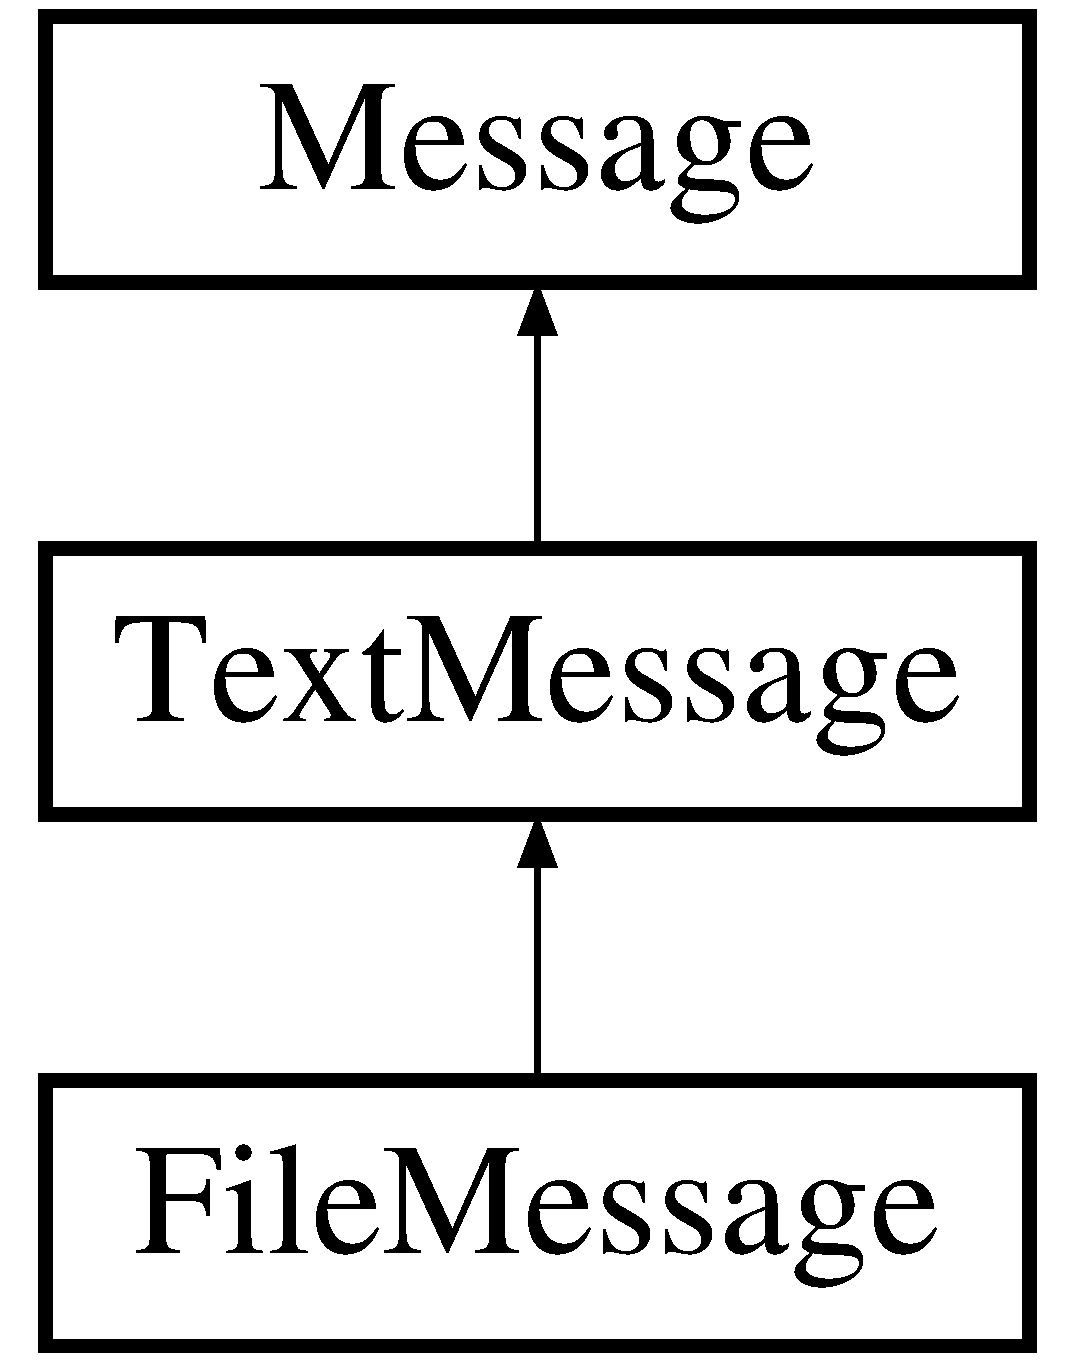
\includegraphics[height=3.000000cm]{class_file_message}
\end{center}
\end{figure}
\subsection*{Public Member Functions}
\begin{DoxyCompactItemize}
\item 
\mbox{\Hypertarget{class_file_message_a04a932a284d897e4a5412ae2b3a990a9}\label{class_file_message_a04a932a284d897e4a5412ae2b3a990a9}} 
{\bfseries File\+Message} (String recipient, String sender, String msg, String fname)
\item 
\mbox{\Hypertarget{class_file_message_a0b6a6e6b6c3147a474b1eb523f470cfc}\label{class_file_message_a0b6a6e6b6c3147a474b1eb523f470cfc}} 
void {\bfseries set\+File} (String filename)
\item 
\mbox{\Hypertarget{class_file_message_a7a820fde575ed8d0f3dc295717fbbfb8}\label{class_file_message_a7a820fde575ed8d0f3dc295717fbbfb8}} 
void {\bfseries set\+Fname} (String fname)
\item 
\mbox{\Hypertarget{class_file_message_a04db9bc0352aad2ff49d242ed6c4e76b}\label{class_file_message_a04db9bc0352aad2ff49d242ed6c4e76b}} 
File {\bfseries get\+File} ()
\item 
\mbox{\Hypertarget{class_file_message_aa9d74a056bfb3d9870deeab6addd1280}\label{class_file_message_aa9d74a056bfb3d9870deeab6addd1280}} 
String {\bfseries get\+Fname} ()
\item 
\mbox{\Hypertarget{class_file_message_a3286338704a438494c2b54aa300cf163}\label{class_file_message_a3286338704a438494c2b54aa300cf163}} 
void {\bfseries send\+Message} ()
\end{DoxyCompactItemize}
\subsection*{Static Public Member Functions}
\begin{DoxyCompactItemize}
\item 
\mbox{\Hypertarget{class_file_message_ae5e65a8c825bf0183f1dad827abf5e0f}\label{class_file_message_ae5e65a8c825bf0183f1dad827abf5e0f}} 
static void \hyperlink{class_file_message_ae5e65a8c825bf0183f1dad827abf5e0f}{main} (String\mbox{[}$\,$\mbox{]} args)
\begin{DoxyCompactList}\small\item\em Implemented for testing purposes. \end{DoxyCompactList}\end{DoxyCompactItemize}


The documentation for this class was generated from the following file\+:\begin{DoxyCompactItemize}
\item 
readwrite/File\+Message.\+java\end{DoxyCompactItemize}

\hypertarget{class_graph}{}\section{Graph Class Reference}
\label{class_graph}\index{Graph@{Graph}}


The \hyperlink{class_graph}{Graph} class creates a graph using objects from the \hyperlink{class_vertex}{Vertex} class and objects from the \hyperlink{class_edge}{Edge} class.  


\subsection*{Public Member Functions}
\begin{DoxyCompactItemize}
\item 
\mbox{\Hypertarget{class_graph_ab8ccb82fd216cc5a36c3887c6820428f}\label{class_graph_ab8ccb82fd216cc5a36c3887c6820428f}} 
\hyperlink{class_graph_ab8ccb82fd216cc5a36c3887c6820428f}{Graph} ()
\begin{DoxyCompactList}\small\item\em create empty graph \end{DoxyCompactList}\item 
\hyperlink{class_graph_ac1c989504f624086332f46af57861d3a}{Graph} (Array\+List$<$ \hyperlink{class_vertex}{Vertex} $>$ vertices)
\begin{DoxyCompactList}\small\item\em create graph with vertices from an arraylist \end{DoxyCompactList}\item 
boolean \hyperlink{class_graph_a50d13043a91c83bfd9d89a4ba24de12b}{add\+Edge} (\hyperlink{class_vertex}{Vertex} one, \hyperlink{class_vertex}{Vertex} two)
\begin{DoxyCompactList}\small\item\em attempt to add an edge \end{DoxyCompactList}\item 
boolean \hyperlink{class_graph_a7f18a8cf5f6fcf5c391fd02e15c7f46c}{add\+Edge} (\hyperlink{class_vertex}{Vertex} one, \hyperlink{class_vertex}{Vertex} two, int weight)
\begin{DoxyCompactList}\small\item\em returns true if add was successful, false if not successful \end{DoxyCompactList}\item 
boolean \hyperlink{class_graph_a64c719dec9e96b255fcd1a72d7f7b636}{contains\+Edge} (\hyperlink{class_edge}{Edge} e)
\begin{DoxyCompactList}\small\item\em check if an edge has two vertices, if not it is likely to be deleted as it isn\textquotesingle{}t a complete edge \end{DoxyCompactList}\item 
\hyperlink{class_edge}{Edge} \hyperlink{class_graph_a5dc8b9103d5d3fb7647b71df8fd35dbb}{remove\+Edge} (\hyperlink{class_edge}{Edge} e)
\begin{DoxyCompactList}\small\item\em remove edge from graph \end{DoxyCompactList}\item 
boolean \hyperlink{class_graph_aff10c71da13d18adef73c4d20c25c895}{add\+Vertex} (\hyperlink{class_vertex}{Vertex} vertex, boolean overwrite\+Existing)
\begin{DoxyCompactList}\small\item\em add a vertex to the graph, returns true if add successful boolean parameter value should be true if you want to allow the vertex to be overwritten if it already exists \end{DoxyCompactList}\item 
boolean \hyperlink{class_graph_a0380eb64afa8f2264eb2472bf62490a2}{contains\+Vertex} (\hyperlink{class_vertex}{Vertex} vertex)
\begin{DoxyCompactList}\small\item\em check if the vertex is in the graphs vertices hashmap \end{DoxyCompactList}\item 
\hyperlink{class_vertex}{Vertex} \hyperlink{class_graph_a9ec421fd3402f637af8a9e99be3bb72c}{get\+Vertex} (String username)
\begin{DoxyCompactList}\small\item\em returns the vertex from vertices hashmap that has the specified username \end{DoxyCompactList}\item 
\hyperlink{class_vertex}{Vertex} \hyperlink{class_graph_a1253c513b85d91e2c6f60e36863c2fc9}{remove\+Vertex} (String username)
\begin{DoxyCompactList}\small\item\em remove a vertex from the graph based on its username \end{DoxyCompactList}\item 
Set$<$ \hyperlink{class_edge}{Edge} $>$ \hyperlink{class_graph_a292e75a764615c537377c66a1deece30}{get\+Edges} ()
\begin{DoxyCompactList}\small\item\em return set containing all edges of the graph \end{DoxyCompactList}\item 
Array\+List$<$ String $>$ \hyperlink{class_graph_a71fd5502d7ef1fb08f9ef49a3b507cb1}{get\+Friends} (String username)
\begin{DoxyCompactList}\small\item\em returns an arraylist containing the usernames, as strings, of all friends of the specified user \end{DoxyCompactList}\end{DoxyCompactItemize}


\subsection{Detailed Description}
The \hyperlink{class_graph}{Graph} class creates a graph using objects from the \hyperlink{class_vertex}{Vertex} class and objects from the \hyperlink{class_edge}{Edge} class. 

\begin{DoxyAuthor}{Author}
830169 
\end{DoxyAuthor}
\begin{DoxyVersion}{Version}
1.\+0 
\end{DoxyVersion}


\subsection{Constructor \& Destructor Documentation}
\mbox{\Hypertarget{class_graph_ac1c989504f624086332f46af57861d3a}\label{class_graph_ac1c989504f624086332f46af57861d3a}} 
\index{Graph@{Graph}!Graph@{Graph}}
\index{Graph@{Graph}!Graph@{Graph}}
\subsubsection{\texorpdfstring{Graph()}{Graph()}}
{\footnotesize\ttfamily Graph.\+Graph (\begin{DoxyParamCaption}\item[{Array\+List$<$ \hyperlink{class_vertex}{Vertex} $>$}]{vertices }\end{DoxyParamCaption})}



create graph with vertices from an arraylist 


\begin{DoxyParams}{Parameters}
{\em vertices} & an arraylist of vertices at be added to the graph \\
\hline
\end{DoxyParams}


\subsection{Member Function Documentation}
\mbox{\Hypertarget{class_graph_a50d13043a91c83bfd9d89a4ba24de12b}\label{class_graph_a50d13043a91c83bfd9d89a4ba24de12b}} 
\index{Graph@{Graph}!add\+Edge@{add\+Edge}}
\index{add\+Edge@{add\+Edge}!Graph@{Graph}}
\subsubsection{\texorpdfstring{add\+Edge()}{addEdge()}\hspace{0.1cm}{\footnotesize\ttfamily [1/2]}}
{\footnotesize\ttfamily boolean Graph.\+add\+Edge (\begin{DoxyParamCaption}\item[{\hyperlink{class_vertex}{Vertex}}]{one,  }\item[{\hyperlink{class_vertex}{Vertex}}]{two }\end{DoxyParamCaption})}



attempt to add an edge 


\begin{DoxyParams}{Parameters}
{\em one} & a first vertex to create edge between \\
\hline
{\em two} & a second vertex to create edge between \\
\hline
\end{DoxyParams}
\begin{DoxyReturn}{Returns}
a boolean that is true if the add was successful 
\end{DoxyReturn}
\mbox{\Hypertarget{class_graph_a7f18a8cf5f6fcf5c391fd02e15c7f46c}\label{class_graph_a7f18a8cf5f6fcf5c391fd02e15c7f46c}} 
\index{Graph@{Graph}!add\+Edge@{add\+Edge}}
\index{add\+Edge@{add\+Edge}!Graph@{Graph}}
\subsubsection{\texorpdfstring{add\+Edge()}{addEdge()}\hspace{0.1cm}{\footnotesize\ttfamily [2/2]}}
{\footnotesize\ttfamily boolean Graph.\+add\+Edge (\begin{DoxyParamCaption}\item[{\hyperlink{class_vertex}{Vertex}}]{one,  }\item[{\hyperlink{class_vertex}{Vertex}}]{two,  }\item[{int}]{weight }\end{DoxyParamCaption})}



returns true if add was successful, false if not successful 


\begin{DoxyParams}{Parameters}
{\em one} & a first vertex to create edge between \\
\hline
{\em two} & a second vertex to create edge between \\
\hline
{\em weight} & the weight of the edge \\
\hline
\end{DoxyParams}
\mbox{\Hypertarget{class_graph_aff10c71da13d18adef73c4d20c25c895}\label{class_graph_aff10c71da13d18adef73c4d20c25c895}} 
\index{Graph@{Graph}!add\+Vertex@{add\+Vertex}}
\index{add\+Vertex@{add\+Vertex}!Graph@{Graph}}
\subsubsection{\texorpdfstring{add\+Vertex()}{addVertex()}}
{\footnotesize\ttfamily boolean Graph.\+add\+Vertex (\begin{DoxyParamCaption}\item[{\hyperlink{class_vertex}{Vertex}}]{vertex,  }\item[{boolean}]{overwrite\+Existing }\end{DoxyParamCaption})}



add a vertex to the graph, returns true if add successful boolean parameter value should be true if you want to allow the vertex to be overwritten if it already exists 


\begin{DoxyParams}{Parameters}
{\em vertex} & the vertex to be added to graph \\
\hline
{\em over\+Write\+Existing} & true = allow overwriting if vertex already exists \\
\hline
\end{DoxyParams}
\begin{DoxyReturn}{Returns}
returns true if the vertex was added successfully, false otherwise 
\end{DoxyReturn}
\mbox{\Hypertarget{class_graph_a64c719dec9e96b255fcd1a72d7f7b636}\label{class_graph_a64c719dec9e96b255fcd1a72d7f7b636}} 
\index{Graph@{Graph}!contains\+Edge@{contains\+Edge}}
\index{contains\+Edge@{contains\+Edge}!Graph@{Graph}}
\subsubsection{\texorpdfstring{contains\+Edge()}{containsEdge()}}
{\footnotesize\ttfamily boolean Graph.\+contains\+Edge (\begin{DoxyParamCaption}\item[{\hyperlink{class_edge}{Edge}}]{e }\end{DoxyParamCaption})}



check if an edge has two vertices, if not it is likely to be deleted as it isn\textquotesingle{}t a complete edge 


\begin{DoxyParams}{Parameters}
{\em e} & edge being searched for \\
\hline
\end{DoxyParams}
\begin{DoxyReturn}{Returns}
true if the edge has two vertices, false otherwise 
\end{DoxyReturn}
\mbox{\Hypertarget{class_graph_a0380eb64afa8f2264eb2472bf62490a2}\label{class_graph_a0380eb64afa8f2264eb2472bf62490a2}} 
\index{Graph@{Graph}!contains\+Vertex@{contains\+Vertex}}
\index{contains\+Vertex@{contains\+Vertex}!Graph@{Graph}}
\subsubsection{\texorpdfstring{contains\+Vertex()}{containsVertex()}}
{\footnotesize\ttfamily boolean Graph.\+contains\+Vertex (\begin{DoxyParamCaption}\item[{\hyperlink{class_vertex}{Vertex}}]{vertex }\end{DoxyParamCaption})}



check if the vertex is in the graphs vertices hashmap 


\begin{DoxyParams}{Parameters}
{\em vertex} & the vertex being searched for \\
\hline
\end{DoxyParams}
\begin{DoxyReturn}{Returns}
returns true if the vertex is in the graph 
\end{DoxyReturn}
\mbox{\Hypertarget{class_graph_a292e75a764615c537377c66a1deece30}\label{class_graph_a292e75a764615c537377c66a1deece30}} 
\index{Graph@{Graph}!get\+Edges@{get\+Edges}}
\index{get\+Edges@{get\+Edges}!Graph@{Graph}}
\subsubsection{\texorpdfstring{get\+Edges()}{getEdges()}}
{\footnotesize\ttfamily Set$<$\hyperlink{class_edge}{Edge}$>$ Graph.\+get\+Edges (\begin{DoxyParamCaption}{ }\end{DoxyParamCaption})}



return set containing all edges of the graph 

\begin{DoxyReturn}{Returns}
a set containing all edges of the graph 
\end{DoxyReturn}
\mbox{\Hypertarget{class_graph_a71fd5502d7ef1fb08f9ef49a3b507cb1}\label{class_graph_a71fd5502d7ef1fb08f9ef49a3b507cb1}} 
\index{Graph@{Graph}!get\+Friends@{get\+Friends}}
\index{get\+Friends@{get\+Friends}!Graph@{Graph}}
\subsubsection{\texorpdfstring{get\+Friends()}{getFriends()}}
{\footnotesize\ttfamily Array\+List$<$String$>$ Graph.\+get\+Friends (\begin{DoxyParamCaption}\item[{String}]{username }\end{DoxyParamCaption})}



returns an arraylist containing the usernames, as strings, of all friends of the specified user 


\begin{DoxyParams}{Parameters}
{\em username} & the username of the person whose friends are being searched for \\
\hline
\end{DoxyParams}
\begin{DoxyReturn}{Returns}
an arraylist containing usernames as strings 
\end{DoxyReturn}
\mbox{\Hypertarget{class_graph_a9ec421fd3402f637af8a9e99be3bb72c}\label{class_graph_a9ec421fd3402f637af8a9e99be3bb72c}} 
\index{Graph@{Graph}!get\+Vertex@{get\+Vertex}}
\index{get\+Vertex@{get\+Vertex}!Graph@{Graph}}
\subsubsection{\texorpdfstring{get\+Vertex()}{getVertex()}}
{\footnotesize\ttfamily \hyperlink{class_vertex}{Vertex} Graph.\+get\+Vertex (\begin{DoxyParamCaption}\item[{String}]{username }\end{DoxyParamCaption})}



returns the vertex from vertices hashmap that has the specified username 


\begin{DoxyParams}{Parameters}
{\em username} & the username of the vertex being searched for \\
\hline
\end{DoxyParams}
\begin{DoxyReturn}{Returns}
the vertex that was searched for by its username 
\end{DoxyReturn}
\mbox{\Hypertarget{class_graph_a5dc8b9103d5d3fb7647b71df8fd35dbb}\label{class_graph_a5dc8b9103d5d3fb7647b71df8fd35dbb}} 
\index{Graph@{Graph}!remove\+Edge@{remove\+Edge}}
\index{remove\+Edge@{remove\+Edge}!Graph@{Graph}}
\subsubsection{\texorpdfstring{remove\+Edge()}{removeEdge()}}
{\footnotesize\ttfamily \hyperlink{class_edge}{Edge} Graph.\+remove\+Edge (\begin{DoxyParamCaption}\item[{\hyperlink{class_edge}{Edge}}]{e }\end{DoxyParamCaption})}



remove edge from graph 


\begin{DoxyParams}{Parameters}
{\em e} & edge to be removed \\
\hline
\end{DoxyParams}
\begin{DoxyReturn}{Returns}
the edge that has been removed 
\end{DoxyReturn}
\mbox{\Hypertarget{class_graph_a1253c513b85d91e2c6f60e36863c2fc9}\label{class_graph_a1253c513b85d91e2c6f60e36863c2fc9}} 
\index{Graph@{Graph}!remove\+Vertex@{remove\+Vertex}}
\index{remove\+Vertex@{remove\+Vertex}!Graph@{Graph}}
\subsubsection{\texorpdfstring{remove\+Vertex()}{removeVertex()}}
{\footnotesize\ttfamily \hyperlink{class_vertex}{Vertex} Graph.\+remove\+Vertex (\begin{DoxyParamCaption}\item[{String}]{username }\end{DoxyParamCaption})}



remove a vertex from the graph based on its username 


\begin{DoxyParams}{Parameters}
{\em username} & the username of the vertex to be removed \\
\hline
\end{DoxyParams}
\begin{DoxyReturn}{Returns}
the vertex that was removed from the graph 
\end{DoxyReturn}


The documentation for this class was generated from the following file\+:\begin{DoxyCompactItemize}
\item 
readwrite/Graph.\+java\end{DoxyCompactItemize}

\hypertarget{class_g_u_i}{}\section{G\+UI Class Reference}
\label{class_g_u_i}\index{G\+UI@{G\+UI}}
Inheritance diagram for G\+UI\+:\begin{figure}[H]
\begin{center}
\leavevmode
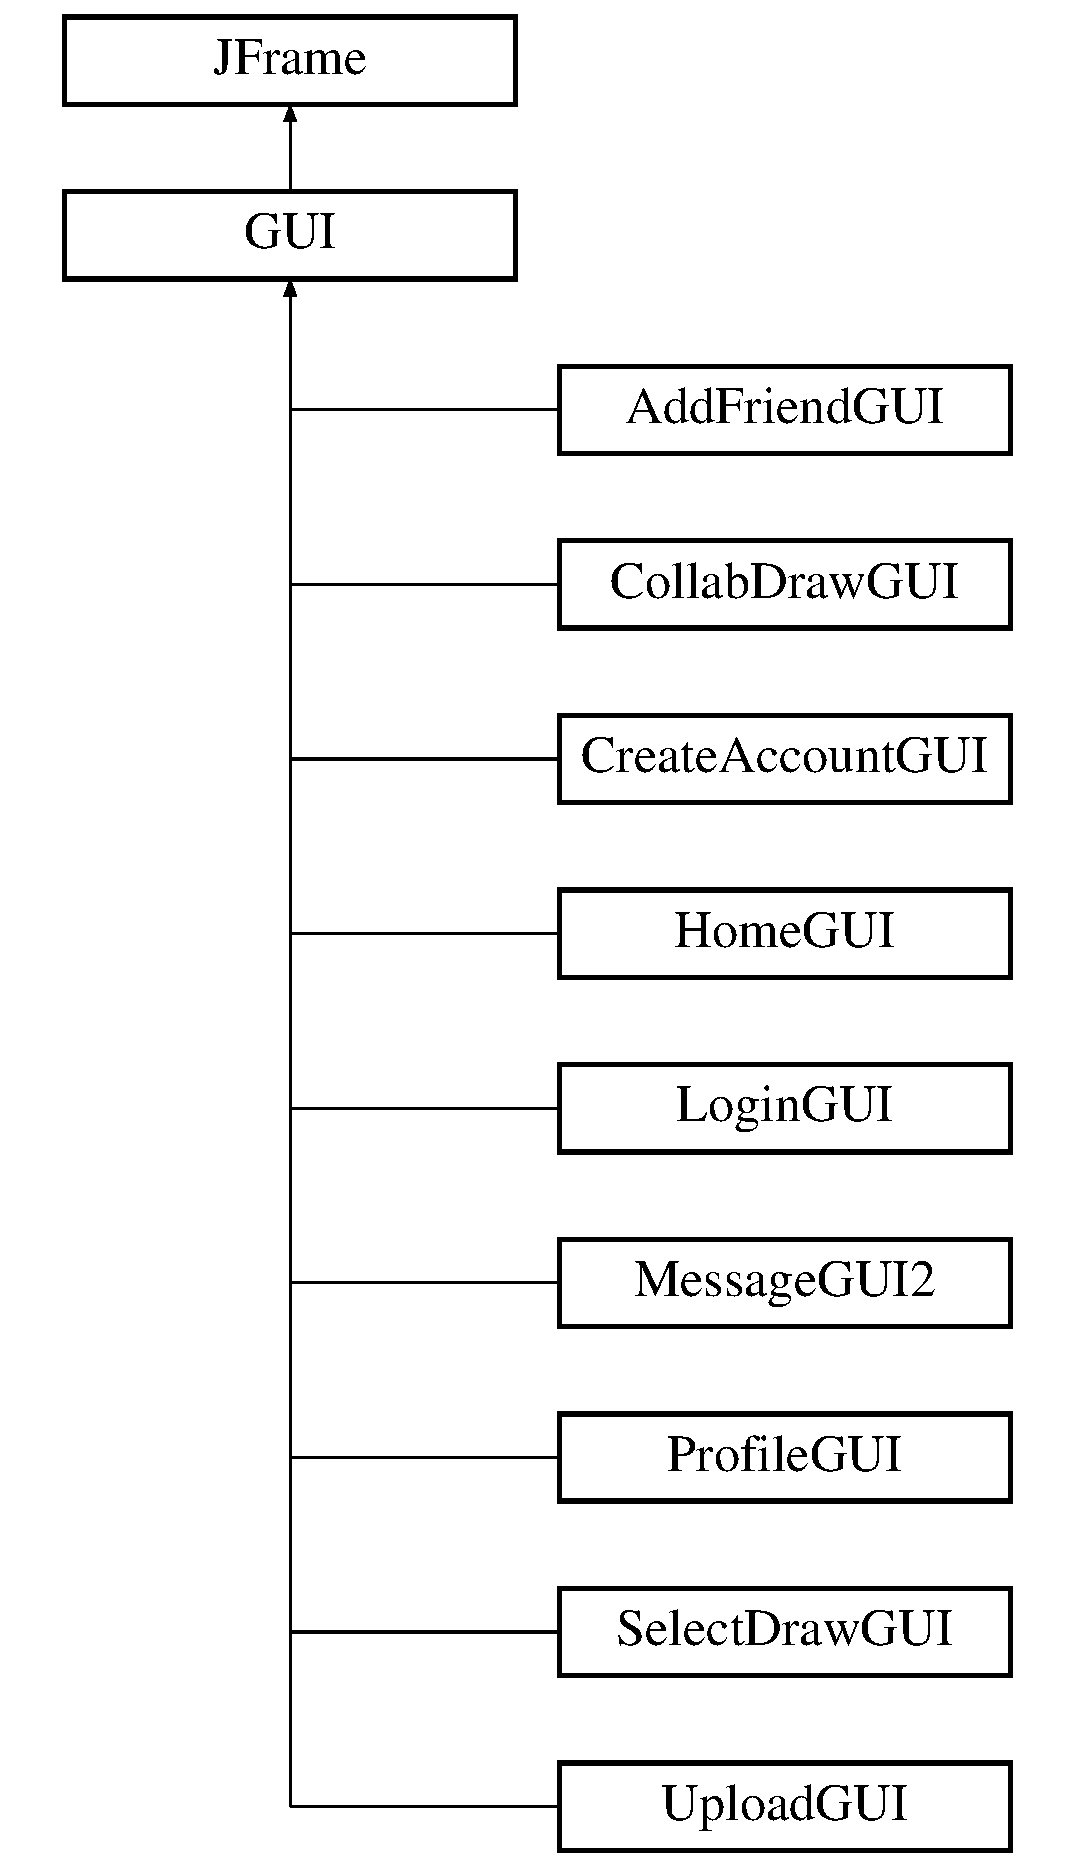
\includegraphics[height=11.000000cm]{class_g_u_i}
\end{center}
\end{figure}
\subsection*{Public Member Functions}
\begin{DoxyCompactItemize}
\item 
\mbox{\Hypertarget{class_g_u_i_a35a15f9dcfca9111335e4401a46567ed}\label{class_g_u_i_a35a15f9dcfca9111335e4401a46567ed}} 
\hyperlink{class_g_u_i_a35a15f9dcfca9111335e4401a46567ed}{G\+UI} ()  throws Exception
\begin{DoxyCompactList}\small\item\em Generates a screen and a toolbar to be used by its subclasses. \end{DoxyCompactList}\item 
\hyperlink{class_main}{Main} \hyperlink{class_g_u_i_abd66813fa465e8cc1f992b250fe1df5b}{get\+\_\+main} ()  throws Exception     
\item 
\mbox{\Hypertarget{class_g_u_i_ab5f498113cffdcfd9f41c026b697acfc}\label{class_g_u_i_ab5f498113cffdcfd9f41c026b697acfc}} 
\hyperlink{class_main}{Main} \hyperlink{class_g_u_i_ab5f498113cffdcfd9f41c026b697acfc}{reset\+\_\+main} ()  throws Exception     
\begin{DoxyCompactList}\small\item\em Resets the \hyperlink{class_main}{Main} class to refresh \hyperlink{class_b_s_t}{B\+ST} and \hyperlink{class_graph}{Graph}. \end{DoxyCompactList}\end{DoxyCompactItemize}
\subsection*{Static Public Member Functions}
\begin{DoxyCompactItemize}
\item 
\mbox{\Hypertarget{class_g_u_i_a8202c223d5b25c7dd94ce70bd6a267ac}\label{class_g_u_i_a8202c223d5b25c7dd94ce70bd6a267ac}} 
static void \hyperlink{class_g_u_i_a8202c223d5b25c7dd94ce70bd6a267ac}{main} (String\mbox{[}$\,$\mbox{]} args)  throws Exception 
\begin{DoxyCompactList}\small\item\em Implemented for testing purposes. \end{DoxyCompactList}\end{DoxyCompactItemize}


\subsection{Member Function Documentation}
\mbox{\Hypertarget{class_g_u_i_abd66813fa465e8cc1f992b250fe1df5b}\label{class_g_u_i_abd66813fa465e8cc1f992b250fe1df5b}} 
\index{G\+UI@{G\+UI}!get\+\_\+main@{get\+\_\+main}}
\index{get\+\_\+main@{get\+\_\+main}!G\+UI@{G\+UI}}
\subsubsection{\texorpdfstring{get\+\_\+main()}{get\_main()}}
{\footnotesize\ttfamily \hyperlink{class_main}{Main} G\+U\+I.\+get\+\_\+main (\begin{DoxyParamCaption}{ }\end{DoxyParamCaption}) throws Exception}

\begin{DoxyReturn}{Returns}
reference to the main file 
\end{DoxyReturn}


The documentation for this class was generated from the following file\+:\begin{DoxyCompactItemize}
\item 
readwrite/G\+U\+I.\+java\end{DoxyCompactItemize}

\hypertarget{class_home_g_u_i}{}\section{Home\+G\+UI Class Reference}
\label{class_home_g_u_i}\index{Home\+G\+UI@{Home\+G\+UI}}
Inheritance diagram for Home\+G\+UI\+:\begin{figure}[H]
\begin{center}
\leavevmode
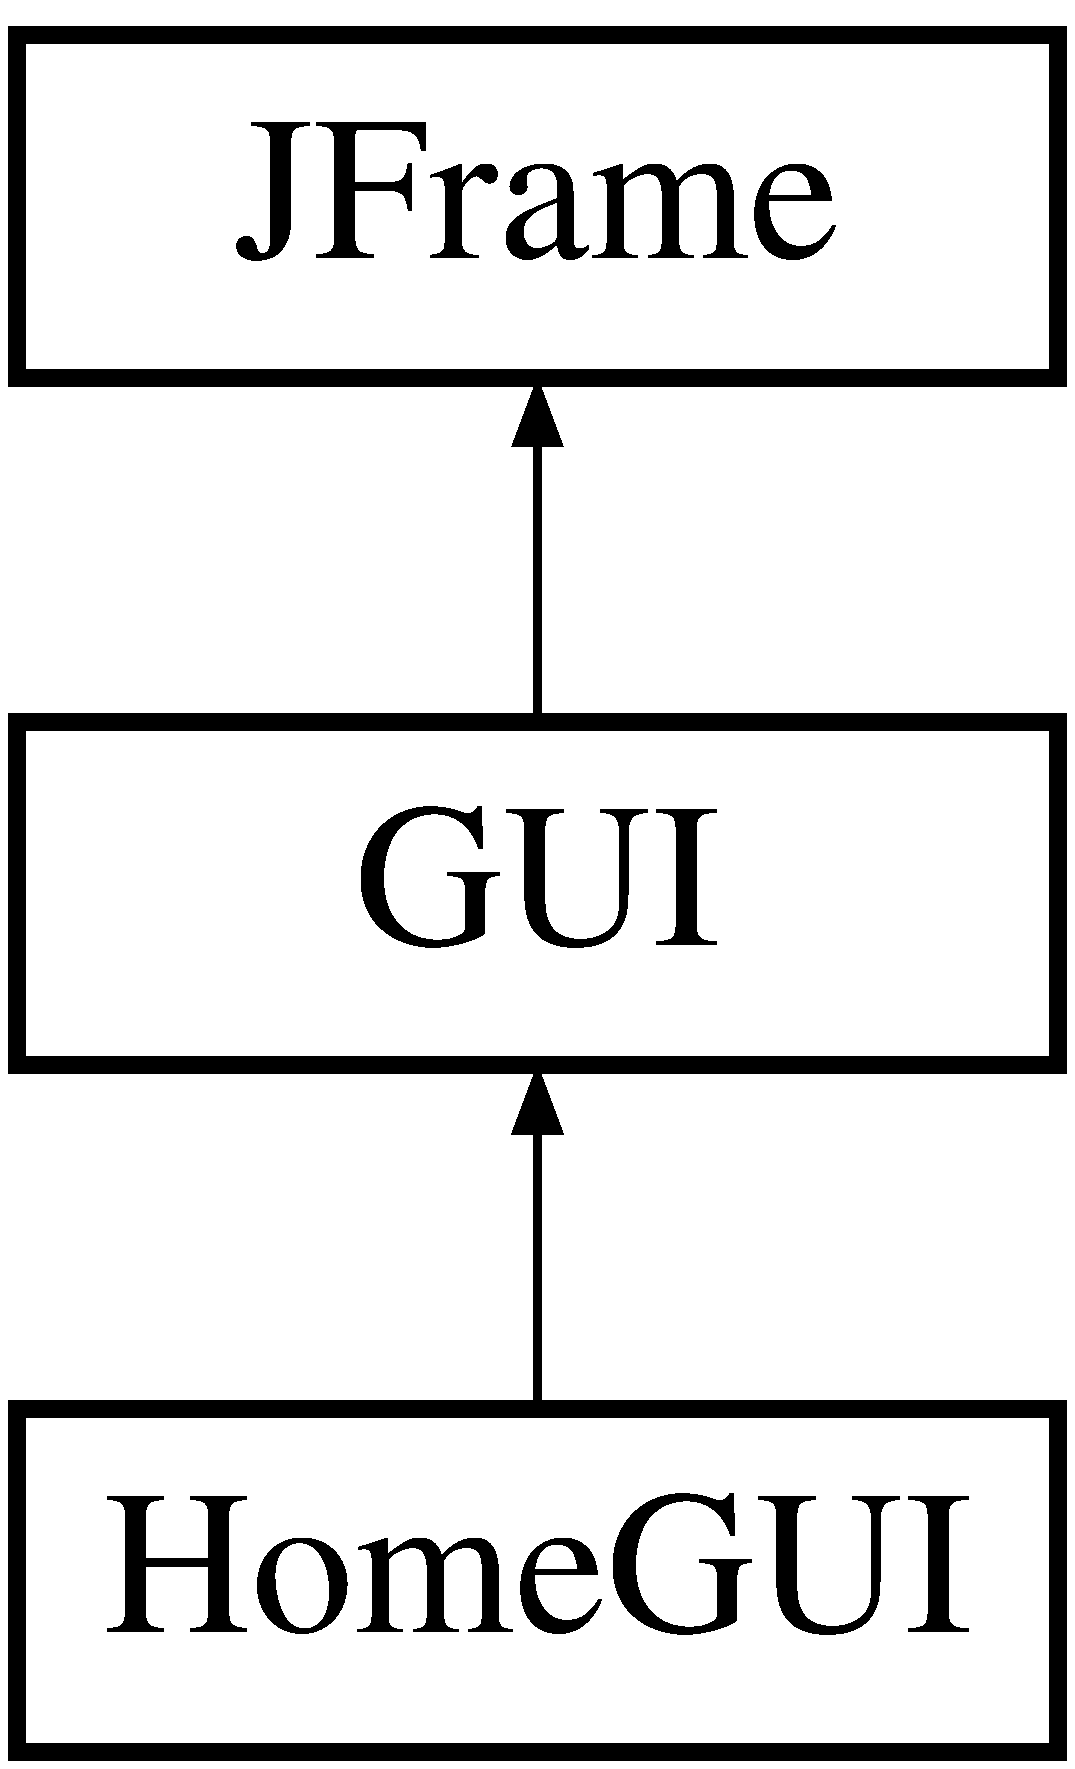
\includegraphics[height=3.000000cm]{class_home_g_u_i}
\end{center}
\end{figure}
\subsection*{Public Member Functions}
\begin{DoxyCompactItemize}
\item 
\mbox{\Hypertarget{class_home_g_u_i_ad0d85d5fd78eab3c47e757d4c7b9859d}\label{class_home_g_u_i_ad0d85d5fd78eab3c47e757d4c7b9859d}} 
{\bfseries Home\+G\+UI} (\hyperlink{class_account}{Account} acc)  throws Exception 
\item 
\mbox{\Hypertarget{class_home_g_u_i_ae36a24898b4b5eefde0f368b34c034ba}\label{class_home_g_u_i_ae36a24898b4b5eefde0f368b34c034ba}} 
void {\bfseries homesetup} (\hyperlink{class_account}{Account} acc)  throws Exception
\end{DoxyCompactItemize}
\subsection*{Static Public Member Functions}
\begin{DoxyCompactItemize}
\item 
\mbox{\Hypertarget{class_home_g_u_i_a103b19a63dc812afce33988dd2cce460}\label{class_home_g_u_i_a103b19a63dc812afce33988dd2cce460}} 
static void {\bfseries main} (String\mbox{[}$\,$\mbox{]} args)  throws Exception 
\end{DoxyCompactItemize}


The documentation for this class was generated from the following file\+:\begin{DoxyCompactItemize}
\item 
readwrite/\hyperlink{_home_g_u_i_8java}{Home\+G\+U\+I.\+java}\end{DoxyCompactItemize}

\hypertarget{class_line}{}\section{Line Class Reference}
\label{class_line}\index{Line@{Line}}
\subsection*{Public Member Functions}
\begin{DoxyCompactItemize}
\item 
\hyperlink{class_line_ad755514ead24f208bd7d7734a1e6aa59}{Line} (int x, int y, int x1, int y1, Color colour)
\begin{DoxyCompactList}\small\item\em Constructor\+: Creates a new \hyperlink{class_line}{Line} object. \end{DoxyCompactList}\item 
int \hyperlink{class_line_a1a555bf02c6b9f7df22558f0717aa651}{get\+StartX} ()
\begin{DoxyCompactList}\small\item\em Method to retrieve the starting X coordinate of the line. \end{DoxyCompactList}\item 
int \hyperlink{class_line_a41eea486d4123a77525ea3b9e95c60af}{get\+StartY} ()
\begin{DoxyCompactList}\small\item\em Method to retrieve the starting Y coordinate of the line. \end{DoxyCompactList}\item 
int \hyperlink{class_line_a7a5d82d47496f42297c77dc359d45e75}{get\+EndX} ()
\begin{DoxyCompactList}\small\item\em Method to retrieve the finishing X coordinate of the line. \end{DoxyCompactList}\item 
int \hyperlink{class_line_add8c48f0c1ee6de19e50dc463502a8ca}{get\+EndY} ()
\begin{DoxyCompactList}\small\item\em Method to retrieve the finishing Y coordinate of the line. \end{DoxyCompactList}\item 
Color \hyperlink{class_line_ab71501e12b598fe6d2adbf5a8a7928e0}{get\+Colour} ()
\begin{DoxyCompactList}\small\item\em Method to retrieve the colour of the line. \end{DoxyCompactList}\end{DoxyCompactItemize}


\subsection{Constructor \& Destructor Documentation}
\mbox{\Hypertarget{class_line_ad755514ead24f208bd7d7734a1e6aa59}\label{class_line_ad755514ead24f208bd7d7734a1e6aa59}} 
\index{Line@{Line}!Line@{Line}}
\index{Line@{Line}!Line@{Line}}
\subsubsection{\texorpdfstring{Line()}{Line()}}
{\footnotesize\ttfamily Line.\+Line (\begin{DoxyParamCaption}\item[{int}]{x,  }\item[{int}]{y,  }\item[{int}]{x1,  }\item[{int}]{y1,  }\item[{Color}]{colour }\end{DoxyParamCaption})}



Constructor\+: Creates a new \hyperlink{class_line}{Line} object. 


\begin{DoxyParams}{Parameters}
{\em x} & -\/ the x coordinate at the start of the line \\
\hline
{\em y} & -\/ the y coordinate at the start of the line \\
\hline
{\em x1} & -\/ the x coordinate at the end of the line \\
\hline
{\em y1} & -\/ the y coordinate at the end of the line \\
\hline
{\em colour} & -\/ the colour of the line \\
\hline
\end{DoxyParams}


\subsection{Member Function Documentation}
\mbox{\Hypertarget{class_line_ab71501e12b598fe6d2adbf5a8a7928e0}\label{class_line_ab71501e12b598fe6d2adbf5a8a7928e0}} 
\index{Line@{Line}!get\+Colour@{get\+Colour}}
\index{get\+Colour@{get\+Colour}!Line@{Line}}
\subsubsection{\texorpdfstring{get\+Colour()}{getColour()}}
{\footnotesize\ttfamily Color Line.\+get\+Colour (\begin{DoxyParamCaption}{ }\end{DoxyParamCaption})}



Method to retrieve the colour of the line. 

\begin{DoxyReturn}{Returns}
a colour object representing the colour. 
\end{DoxyReturn}
\mbox{\Hypertarget{class_line_a7a5d82d47496f42297c77dc359d45e75}\label{class_line_a7a5d82d47496f42297c77dc359d45e75}} 
\index{Line@{Line}!get\+EndX@{get\+EndX}}
\index{get\+EndX@{get\+EndX}!Line@{Line}}
\subsubsection{\texorpdfstring{get\+End\+X()}{getEndX()}}
{\footnotesize\ttfamily int Line.\+get\+EndX (\begin{DoxyParamCaption}{ }\end{DoxyParamCaption})}



Method to retrieve the finishing X coordinate of the line. 

\begin{DoxyReturn}{Returns}
an int representing the x coordinate. 
\end{DoxyReturn}
\mbox{\Hypertarget{class_line_add8c48f0c1ee6de19e50dc463502a8ca}\label{class_line_add8c48f0c1ee6de19e50dc463502a8ca}} 
\index{Line@{Line}!get\+EndY@{get\+EndY}}
\index{get\+EndY@{get\+EndY}!Line@{Line}}
\subsubsection{\texorpdfstring{get\+End\+Y()}{getEndY()}}
{\footnotesize\ttfamily int Line.\+get\+EndY (\begin{DoxyParamCaption}{ }\end{DoxyParamCaption})}



Method to retrieve the finishing Y coordinate of the line. 

\begin{DoxyReturn}{Returns}
an int representing the y coordinate. 
\end{DoxyReturn}
\mbox{\Hypertarget{class_line_a1a555bf02c6b9f7df22558f0717aa651}\label{class_line_a1a555bf02c6b9f7df22558f0717aa651}} 
\index{Line@{Line}!get\+StartX@{get\+StartX}}
\index{get\+StartX@{get\+StartX}!Line@{Line}}
\subsubsection{\texorpdfstring{get\+Start\+X()}{getStartX()}}
{\footnotesize\ttfamily int Line.\+get\+StartX (\begin{DoxyParamCaption}{ }\end{DoxyParamCaption})}



Method to retrieve the starting X coordinate of the line. 

\begin{DoxyReturn}{Returns}
an int representing the x coordinate. 
\end{DoxyReturn}
\mbox{\Hypertarget{class_line_a41eea486d4123a77525ea3b9e95c60af}\label{class_line_a41eea486d4123a77525ea3b9e95c60af}} 
\index{Line@{Line}!get\+StartY@{get\+StartY}}
\index{get\+StartY@{get\+StartY}!Line@{Line}}
\subsubsection{\texorpdfstring{get\+Start\+Y()}{getStartY()}}
{\footnotesize\ttfamily int Line.\+get\+StartY (\begin{DoxyParamCaption}{ }\end{DoxyParamCaption})}



Method to retrieve the starting Y coordinate of the line. 

\begin{DoxyReturn}{Returns}
an int representing the y coordinate. 
\end{DoxyReturn}


The documentation for this class was generated from the following file\+:\begin{DoxyCompactItemize}
\item 
readwrite/Line.\+java\end{DoxyCompactItemize}

\hypertarget{class_login_g_u_i}{}\section{Login\+G\+UI Class Reference}
\label{class_login_g_u_i}\index{Login\+G\+UI@{Login\+G\+UI}}
Inheritance diagram for Login\+G\+UI\+:\begin{figure}[H]
\begin{center}
\leavevmode
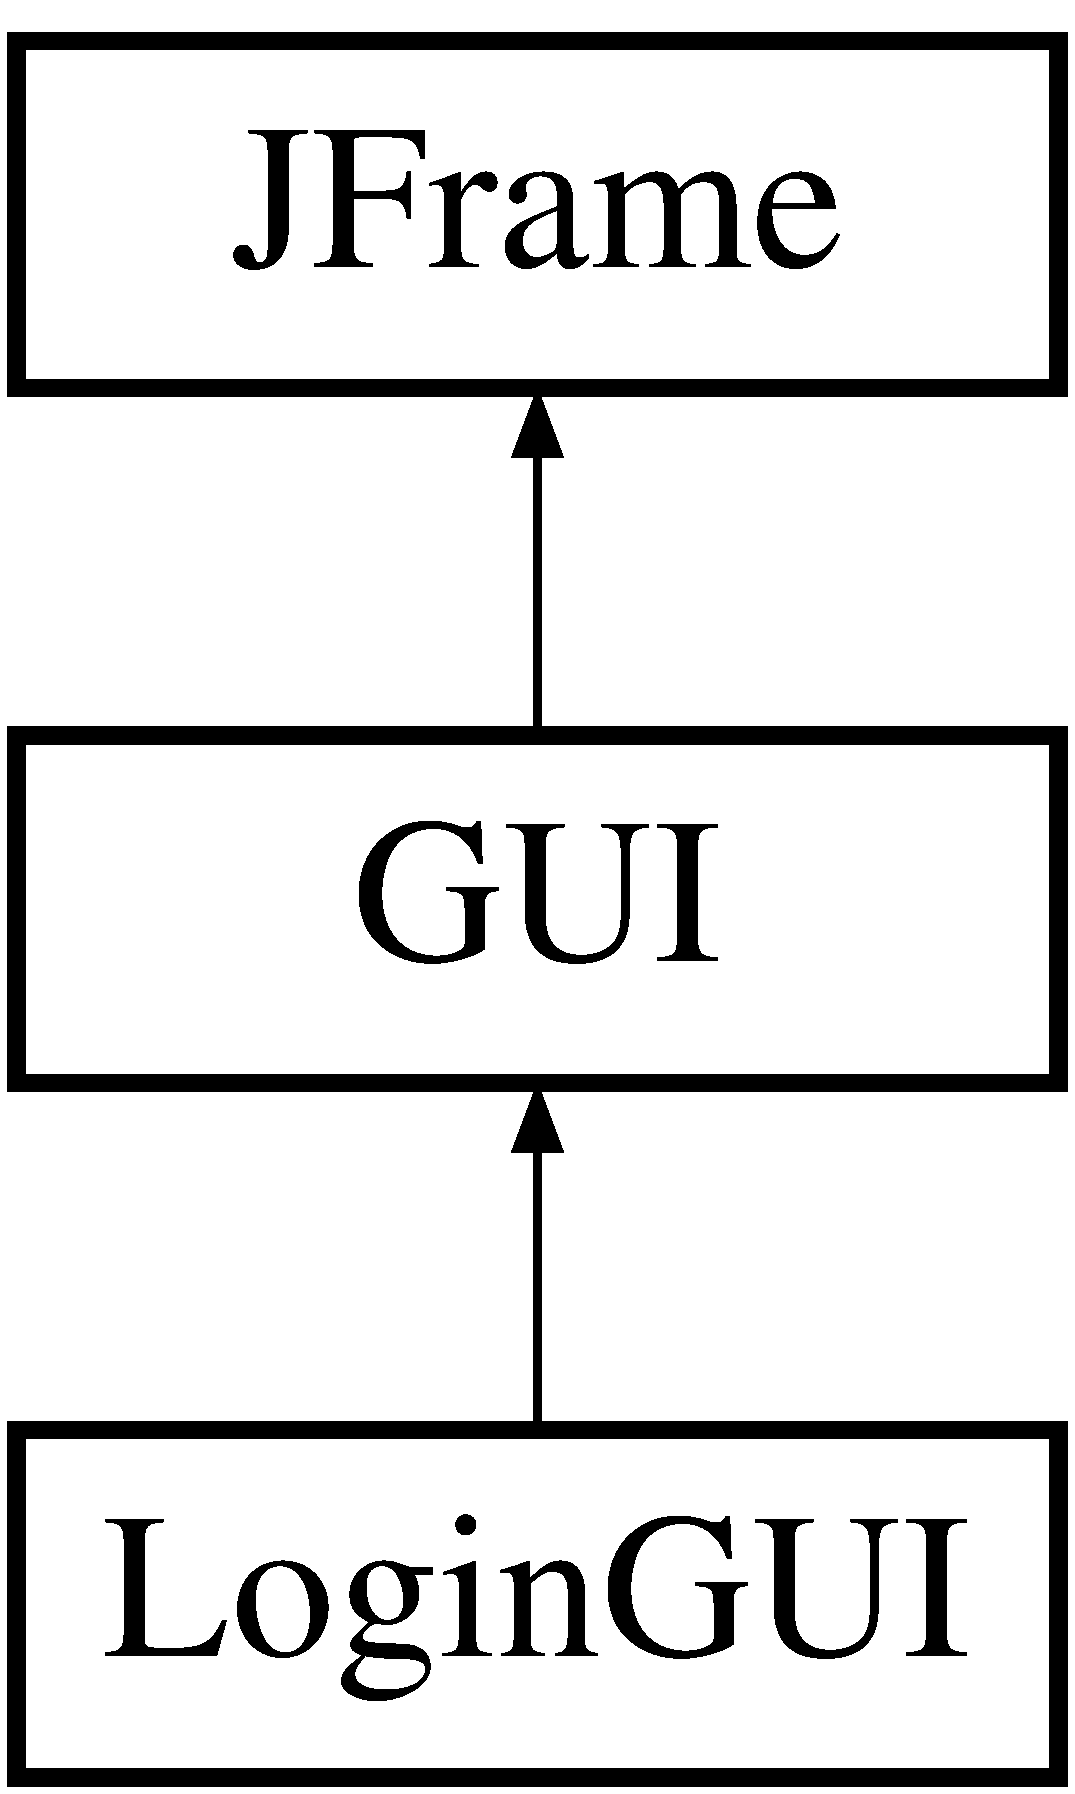
\includegraphics[height=3.000000cm]{class_login_g_u_i}
\end{center}
\end{figure}
\subsection*{Public Member Functions}
\begin{DoxyCompactItemize}
\item 
\mbox{\Hypertarget{class_login_g_u_i_a37fd25505687793a026b91708cbb2d1a}\label{class_login_g_u_i_a37fd25505687793a026b91708cbb2d1a}} 
\hyperlink{class_login_g_u_i_a37fd25505687793a026b91708cbb2d1a}{Login\+G\+UI} ()  throws Exception 
\begin{DoxyCompactList}\small\item\em Builds the window and handles if a user exists in the system using the \hyperlink{class_b_s_t}{B\+ST}. \end{DoxyCompactList}\end{DoxyCompactItemize}
\subsection*{Static Public Member Functions}
\begin{DoxyCompactItemize}
\item 
\mbox{\Hypertarget{class_login_g_u_i_a4b8e369327f04ab3c9fb11886c5f1dbb}\label{class_login_g_u_i_a4b8e369327f04ab3c9fb11886c5f1dbb}} 
static void \hyperlink{class_login_g_u_i_a4b8e369327f04ab3c9fb11886c5f1dbb}{main} (String\mbox{[}$\,$\mbox{]} args)  throws Exception 	
\begin{DoxyCompactList}\small\item\em Implemented for testing purposes. \end{DoxyCompactList}\end{DoxyCompactItemize}


The documentation for this class was generated from the following file\+:\begin{DoxyCompactItemize}
\item 
readwrite/Login\+G\+U\+I.\+java\end{DoxyCompactItemize}

\hypertarget{class_main}{}\section{Main Class Reference}
\label{class_main}\index{Main@{Main}}
\subsection*{Public Member Functions}
\begin{DoxyCompactItemize}
\item 
\mbox{\Hypertarget{class_main_a86df60b74e5d667547357dc7935b4b70}\label{class_main_a86df60b74e5d667547357dc7935b4b70}} 
\hyperlink{class_main_a86df60b74e5d667547357dc7935b4b70}{Main} ()  throws Exception     
\begin{DoxyCompactList}\small\item\em Generates the \hyperlink{class_b_s_t}{B\+ST} and \hyperlink{class_graph}{Graph}, populating them with information from the \hyperlink{class_read_write_account}{Read\+Write\+Account} and \hyperlink{class_read_write_friends}{Read\+Write\+Friends} classes. \end{DoxyCompactList}\item 
\mbox{\Hypertarget{class_main_a61851ea3ba57eaaff107ae9e3c053f2e}\label{class_main_a61851ea3ba57eaaff107ae9e3c053f2e}} 
\hyperlink{class_b_s_t}{B\+ST} \hyperlink{class_main_a61851ea3ba57eaaff107ae9e3c053f2e}{populate\+\_\+tree} (\hyperlink{class_b_s_t}{B\+ST} tree, Array\+List$<$ \hyperlink{class_account}{Account} $>$ acc)  throws Exception     
\begin{DoxyCompactList}\small\item\em Populates a \hyperlink{class_b_s_t}{B\+ST} with Accounts from the database. \end{DoxyCompactList}\item 
\hyperlink{class_graph}{Graph} \hyperlink{class_main_a5fd22f13b47ed4f7f56283461f2d8738}{populate\+\_\+graph} (\hyperlink{class_graph}{Graph} graph, Array\+List$<$ \hyperlink{class_account}{Account} $>$ acc)  throws Exception     
\begin{DoxyCompactList}\small\item\em Populates the graph with friendship information. \end{DoxyCompactList}\item 
\mbox{\Hypertarget{class_main_a42d61a73dcc88d218eb16a9e72dd77b1}\label{class_main_a42d61a73dcc88d218eb16a9e72dd77b1}} 
\hyperlink{class_graph}{Graph} {\bfseries get\+\_\+graph} ()
\item 
\mbox{\Hypertarget{class_main_a97b7b2054c74f0789a4026bacb3d308a}\label{class_main_a97b7b2054c74f0789a4026bacb3d308a}} 
\hyperlink{class_b_s_t}{B\+ST} {\bfseries get\+\_\+tree} ()
\end{DoxyCompactItemize}
\subsection*{Static Public Member Functions}
\begin{DoxyCompactItemize}
\item 
static \hyperlink{class_login_g_u_i}{Login\+G\+UI} \hyperlink{class_main_adbc9a9d0ef627e04ed81e7e61689dc01}{get\+\_\+login} ()  throws Exception     
\item 
static \hyperlink{class_message_g_u_i2}{Message\+G\+U\+I2} \hyperlink{class_main_a21b6962a0baf060031b59f4966ff6abf}{get\+\_\+message} ()  throws Exception     
\item 
static \hyperlink{class_create_account_g_u_i}{Create\+Account\+G\+UI} \hyperlink{class_main_a0d47d64d3fd1d384ca1e9327d614e700}{get\+\_\+create} ()  throws Exception     
\item 
static \hyperlink{class_home_g_u_i}{Home\+G\+UI} \hyperlink{class_main_a59e90cad9e7b3a6dc7e6f3ff60461552}{get\+\_\+home} ()  throws Exception     
\item 
static \hyperlink{class_profile_g_u_i}{Profile\+G\+UI} \hyperlink{class_main_a73e8f5786c0c767bdc6f236199bddd70}{get\+\_\+profile} ()  throws Exception     
\item 
static \hyperlink{class_collab_draw_g_u_i}{Collab\+Draw\+G\+UI} \hyperlink{class_main_a8e7bcb41f4403124bc9bca5018d30e7a}{get\+\_\+draw} ()  throws Exception     
\item 
\mbox{\Hypertarget{class_main_a615e65902105d5888a9050b279c89d80}\label{class_main_a615e65902105d5888a9050b279c89d80}} 
static void \hyperlink{class_main_a615e65902105d5888a9050b279c89d80}{set\+\_\+login} ()  throws Exception     
\begin{DoxyCompactList}\small\item\em Sets up the \hyperlink{class_login_g_u_i}{Login\+G\+UI} variable. \end{DoxyCompactList}\item 
\mbox{\Hypertarget{class_main_a40f46d7ff4e56752d41c9db5e451172f}\label{class_main_a40f46d7ff4e56752d41c9db5e451172f}} 
static void \hyperlink{class_main_a40f46d7ff4e56752d41c9db5e451172f}{set\+\_\+message} (\hyperlink{class_account}{Account} acc)  throws Exception     
\begin{DoxyCompactList}\small\item\em Sets up the \hyperlink{class_message_g_u_i2}{Message\+G\+U\+I2} variable. \end{DoxyCompactList}\item 
\mbox{\Hypertarget{class_main_a34548bd2b4340a9988b3a746954d7d9a}\label{class_main_a34548bd2b4340a9988b3a746954d7d9a}} 
static void \hyperlink{class_main_a34548bd2b4340a9988b3a746954d7d9a}{set\+\_\+create} ()  throws Exception     
\begin{DoxyCompactList}\small\item\em Sets up the \hyperlink{class_create_account_g_u_i}{Create\+Account\+G\+UI} variable. \end{DoxyCompactList}\item 
\mbox{\Hypertarget{class_main_a28021e928cc0f251eaadfe64226890c8}\label{class_main_a28021e928cc0f251eaadfe64226890c8}} 
static void \hyperlink{class_main_a28021e928cc0f251eaadfe64226890c8}{set\+\_\+home} (\hyperlink{class_account}{Account} acc)  throws Exception     
\begin{DoxyCompactList}\small\item\em Sets up the \hyperlink{class_home_g_u_i}{Home\+G\+UI} variable. \end{DoxyCompactList}\item 
\mbox{\Hypertarget{class_main_a97617e73a5156ccc2c900054cdfa3b23}\label{class_main_a97617e73a5156ccc2c900054cdfa3b23}} 
static void \hyperlink{class_main_a97617e73a5156ccc2c900054cdfa3b23}{set\+\_\+profile} (\hyperlink{class_account}{Account} acc)  throws Exception     
\begin{DoxyCompactList}\small\item\em Sets up the \hyperlink{class_profile_g_u_i}{Profile\+G\+UI} variable. \end{DoxyCompactList}\item 
\mbox{\Hypertarget{class_main_a7c2f08652e3be5429bc978707078bed9}\label{class_main_a7c2f08652e3be5429bc978707078bed9}} 
static void \hyperlink{class_main_a7c2f08652e3be5429bc978707078bed9}{set\+\_\+draw} (\hyperlink{class_account}{Account} acc1, \hyperlink{class_account}{Account} acc2)  throws Exception     
\begin{DoxyCompactList}\small\item\em Sets up the \hyperlink{class_collab_draw_g_u_i}{Collab\+Draw\+G\+UI} variable. \end{DoxyCompactList}\item 
\mbox{\Hypertarget{class_main_a8a5d0f827edddff706cc0e6740d0579a}\label{class_main_a8a5d0f827edddff706cc0e6740d0579a}} 
static void \hyperlink{class_main_a8a5d0f827edddff706cc0e6740d0579a}{main} (String\mbox{[}$\,$\mbox{]} args)  throws Exception     
\begin{DoxyCompactList}\small\item\em Here for testing purposes. \end{DoxyCompactList}\end{DoxyCompactItemize}
\subsection*{Static Public Attributes}
\begin{DoxyCompactItemize}
\item 
\mbox{\Hypertarget{class_main_a368d0eacb148dfeeeffc5d85bea45a9a}\label{class_main_a368d0eacb148dfeeeffc5d85bea45a9a}} 
static \hyperlink{class_login_g_u_i}{Login\+G\+UI} {\bfseries login}
\item 
\mbox{\Hypertarget{class_main_af5bdcc4b883ce996098d27d6d189a1e3}\label{class_main_af5bdcc4b883ce996098d27d6d189a1e3}} 
static \hyperlink{class_message_g_u_i2}{Message\+G\+U\+I2} {\bfseries msg}
\item 
\mbox{\Hypertarget{class_main_ad83de0fbeb554341ca2f083b99df8318}\label{class_main_ad83de0fbeb554341ca2f083b99df8318}} 
static \hyperlink{class_create_account_g_u_i}{Create\+Account\+G\+UI} {\bfseries create}
\item 
\mbox{\Hypertarget{class_main_ad944c3306bc966c49dd370baaefd7ed2}\label{class_main_ad944c3306bc966c49dd370baaefd7ed2}} 
static \hyperlink{class_home_g_u_i}{Home\+G\+UI} {\bfseries home}
\item 
\mbox{\Hypertarget{class_main_a7f8a2abcb8b79baf0bf1020a3322f37d}\label{class_main_a7f8a2abcb8b79baf0bf1020a3322f37d}} 
static \hyperlink{class_profile_g_u_i}{Profile\+G\+UI} {\bfseries profile}
\item 
\mbox{\Hypertarget{class_main_a26fc9b293a3101f877720090c1d966d0}\label{class_main_a26fc9b293a3101f877720090c1d966d0}} 
static \hyperlink{class_collab_draw_g_u_i}{Collab\+Draw\+G\+UI} {\bfseries draw}
\end{DoxyCompactItemize}


\subsection{Member Function Documentation}
\mbox{\Hypertarget{class_main_a0d47d64d3fd1d384ca1e9327d614e700}\label{class_main_a0d47d64d3fd1d384ca1e9327d614e700}} 
\index{Main@{Main}!get\+\_\+create@{get\+\_\+create}}
\index{get\+\_\+create@{get\+\_\+create}!Main@{Main}}
\subsubsection{\texorpdfstring{get\+\_\+create()}{get\_create()}}
{\footnotesize\ttfamily static \hyperlink{class_create_account_g_u_i}{Create\+Account\+G\+UI} Main.\+get\+\_\+create (\begin{DoxyParamCaption}{ }\end{DoxyParamCaption}) throws Exception\hspace{0.3cm}{\ttfamily [static]}}

\begin{DoxyReturn}{Returns}
Class variable for \hyperlink{class_create_account_g_u_i}{Create\+Account\+G\+UI} 
\end{DoxyReturn}
\mbox{\Hypertarget{class_main_a8e7bcb41f4403124bc9bca5018d30e7a}\label{class_main_a8e7bcb41f4403124bc9bca5018d30e7a}} 
\index{Main@{Main}!get\+\_\+draw@{get\+\_\+draw}}
\index{get\+\_\+draw@{get\+\_\+draw}!Main@{Main}}
\subsubsection{\texorpdfstring{get\+\_\+draw()}{get\_draw()}}
{\footnotesize\ttfamily static \hyperlink{class_collab_draw_g_u_i}{Collab\+Draw\+G\+UI} Main.\+get\+\_\+draw (\begin{DoxyParamCaption}{ }\end{DoxyParamCaption}) throws Exception\hspace{0.3cm}{\ttfamily [static]}}

\begin{DoxyReturn}{Returns}
Class variable for \hyperlink{class_collab_draw_g_u_i}{Collab\+Draw\+G\+UI} 
\end{DoxyReturn}
\mbox{\Hypertarget{class_main_a59e90cad9e7b3a6dc7e6f3ff60461552}\label{class_main_a59e90cad9e7b3a6dc7e6f3ff60461552}} 
\index{Main@{Main}!get\+\_\+home@{get\+\_\+home}}
\index{get\+\_\+home@{get\+\_\+home}!Main@{Main}}
\subsubsection{\texorpdfstring{get\+\_\+home()}{get\_home()}}
{\footnotesize\ttfamily static \hyperlink{class_home_g_u_i}{Home\+G\+UI} Main.\+get\+\_\+home (\begin{DoxyParamCaption}{ }\end{DoxyParamCaption}) throws Exception\hspace{0.3cm}{\ttfamily [static]}}

\begin{DoxyReturn}{Returns}
Class variable for \hyperlink{class_home_g_u_i}{Home\+G\+UI} 
\end{DoxyReturn}
\mbox{\Hypertarget{class_main_adbc9a9d0ef627e04ed81e7e61689dc01}\label{class_main_adbc9a9d0ef627e04ed81e7e61689dc01}} 
\index{Main@{Main}!get\+\_\+login@{get\+\_\+login}}
\index{get\+\_\+login@{get\+\_\+login}!Main@{Main}}
\subsubsection{\texorpdfstring{get\+\_\+login()}{get\_login()}}
{\footnotesize\ttfamily static \hyperlink{class_login_g_u_i}{Login\+G\+UI} Main.\+get\+\_\+login (\begin{DoxyParamCaption}{ }\end{DoxyParamCaption}) throws Exception\hspace{0.3cm}{\ttfamily [static]}}

\begin{DoxyReturn}{Returns}
Class variable for \hyperlink{class_login_g_u_i}{Login\+G\+UI} 
\end{DoxyReturn}
\mbox{\Hypertarget{class_main_a21b6962a0baf060031b59f4966ff6abf}\label{class_main_a21b6962a0baf060031b59f4966ff6abf}} 
\index{Main@{Main}!get\+\_\+message@{get\+\_\+message}}
\index{get\+\_\+message@{get\+\_\+message}!Main@{Main}}
\subsubsection{\texorpdfstring{get\+\_\+message()}{get\_message()}}
{\footnotesize\ttfamily static \hyperlink{class_message_g_u_i2}{Message\+G\+U\+I2} Main.\+get\+\_\+message (\begin{DoxyParamCaption}{ }\end{DoxyParamCaption}) throws Exception\hspace{0.3cm}{\ttfamily [static]}}

\begin{DoxyReturn}{Returns}
Class variable for \hyperlink{class_message_g_u_i2}{Message\+G\+U\+I2} 
\end{DoxyReturn}
\mbox{\Hypertarget{class_main_a73e8f5786c0c767bdc6f236199bddd70}\label{class_main_a73e8f5786c0c767bdc6f236199bddd70}} 
\index{Main@{Main}!get\+\_\+profile@{get\+\_\+profile}}
\index{get\+\_\+profile@{get\+\_\+profile}!Main@{Main}}
\subsubsection{\texorpdfstring{get\+\_\+profile()}{get\_profile()}}
{\footnotesize\ttfamily static \hyperlink{class_profile_g_u_i}{Profile\+G\+UI} Main.\+get\+\_\+profile (\begin{DoxyParamCaption}{ }\end{DoxyParamCaption}) throws Exception\hspace{0.3cm}{\ttfamily [static]}}

\begin{DoxyReturn}{Returns}
Class variable for \hyperlink{class_profile_g_u_i}{Profile\+G\+UI} 
\end{DoxyReturn}
\mbox{\Hypertarget{class_main_a5fd22f13b47ed4f7f56283461f2d8738}\label{class_main_a5fd22f13b47ed4f7f56283461f2d8738}} 
\index{Main@{Main}!populate\+\_\+graph@{populate\+\_\+graph}}
\index{populate\+\_\+graph@{populate\+\_\+graph}!Main@{Main}}
\subsubsection{\texorpdfstring{populate\+\_\+graph()}{populate\_graph()}}
{\footnotesize\ttfamily \hyperlink{class_graph}{Graph} Main.\+populate\+\_\+graph (\begin{DoxyParamCaption}\item[{\hyperlink{class_graph}{Graph}}]{graph,  }\item[{Array\+List$<$ \hyperlink{class_account}{Account} $>$}]{acc }\end{DoxyParamCaption}) throws Exception}



Populates the graph with friendship information. 


\begin{DoxyParams}{Parameters}
{\em graph} & The graph object we\textquotesingle{}re adding to \\
\hline
{\em acc} & Array\+List of every account in the database \\
\hline
\end{DoxyParams}


The documentation for this class was generated from the following file\+:\begin{DoxyCompactItemize}
\item 
readwrite/Main.\+java\end{DoxyCompactItemize}

\hypertarget{class_message}{}\section{Message Class Reference}
\label{class_message}\index{Message@{Message}}
Inheritance diagram for Message\+:\begin{figure}[H]
\begin{center}
\leavevmode
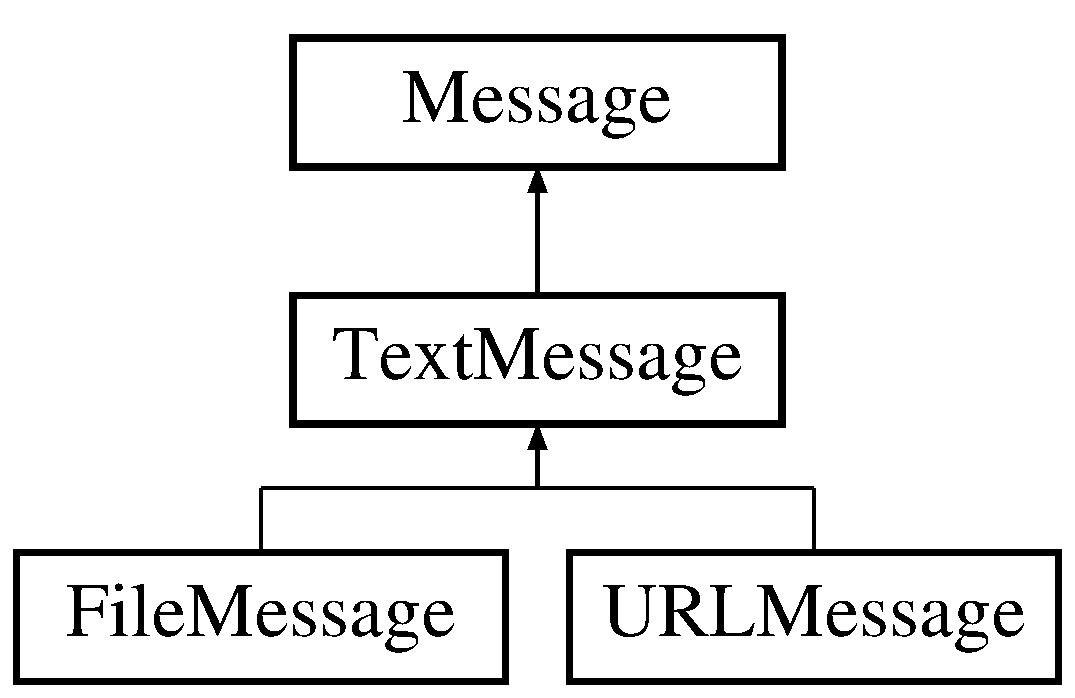
\includegraphics[height=3.000000cm]{class_message}
\end{center}
\end{figure}
\subsection*{Public Member Functions}
\begin{DoxyCompactItemize}
\item 
\mbox{\Hypertarget{class_message_a7c336ac492169c70df799ffdfaf02f2e}\label{class_message_a7c336ac492169c70df799ffdfaf02f2e}} 
{\bfseries Message} (String recipient, String sender)
\item 
\mbox{\Hypertarget{class_message_aa434db00d360b66f170302eb5e650731}\label{class_message_aa434db00d360b66f170302eb5e650731}} 
void {\bfseries set\+Recipient} (String recipient)
\item 
\mbox{\Hypertarget{class_message_ab07abfbf9a9533506caa21a445021064}\label{class_message_ab07abfbf9a9533506caa21a445021064}} 
void {\bfseries set\+Sender} (String sender)
\item 
\mbox{\Hypertarget{class_message_a18cbe1109db77983103d6f6b84c7e0f2}\label{class_message_a18cbe1109db77983103d6f6b84c7e0f2}} 
String {\bfseries get\+Recipient} ()
\item 
\mbox{\Hypertarget{class_message_aa367758d3a7dc4977fe09cd17dffa36a}\label{class_message_aa367758d3a7dc4977fe09cd17dffa36a}} 
String {\bfseries get\+Sender} ()
\item 
\mbox{\Hypertarget{class_message_aad82a5b5042d3ac413769baa1d662846}\label{class_message_aad82a5b5042d3ac413769baa1d662846}} 
void {\bfseries send\+Message} ()
\end{DoxyCompactItemize}
\subsection*{Static Public Member Functions}
\begin{DoxyCompactItemize}
\item 
\mbox{\Hypertarget{class_message_aabda3e5fd7680cf235e10a8fccae8c7a}\label{class_message_aabda3e5fd7680cf235e10a8fccae8c7a}} 
static void \hyperlink{class_message_aabda3e5fd7680cf235e10a8fccae8c7a}{main} (String \mbox{[}$\,$\mbox{]} args)
\begin{DoxyCompactList}\small\item\em Implemented for testing purposes. \end{DoxyCompactList}\end{DoxyCompactItemize}


The documentation for this class was generated from the following file\+:\begin{DoxyCompactItemize}
\item 
readwrite/Message.\+java\end{DoxyCompactItemize}

\hypertarget{class_message_g_u_i2}{}\section{Message\+G\+U\+I2 Class Reference}
\label{class_message_g_u_i2}\index{Message\+G\+U\+I2@{Message\+G\+U\+I2}}
Inheritance diagram for Message\+G\+U\+I2\+:\begin{figure}[H]
\begin{center}
\leavevmode
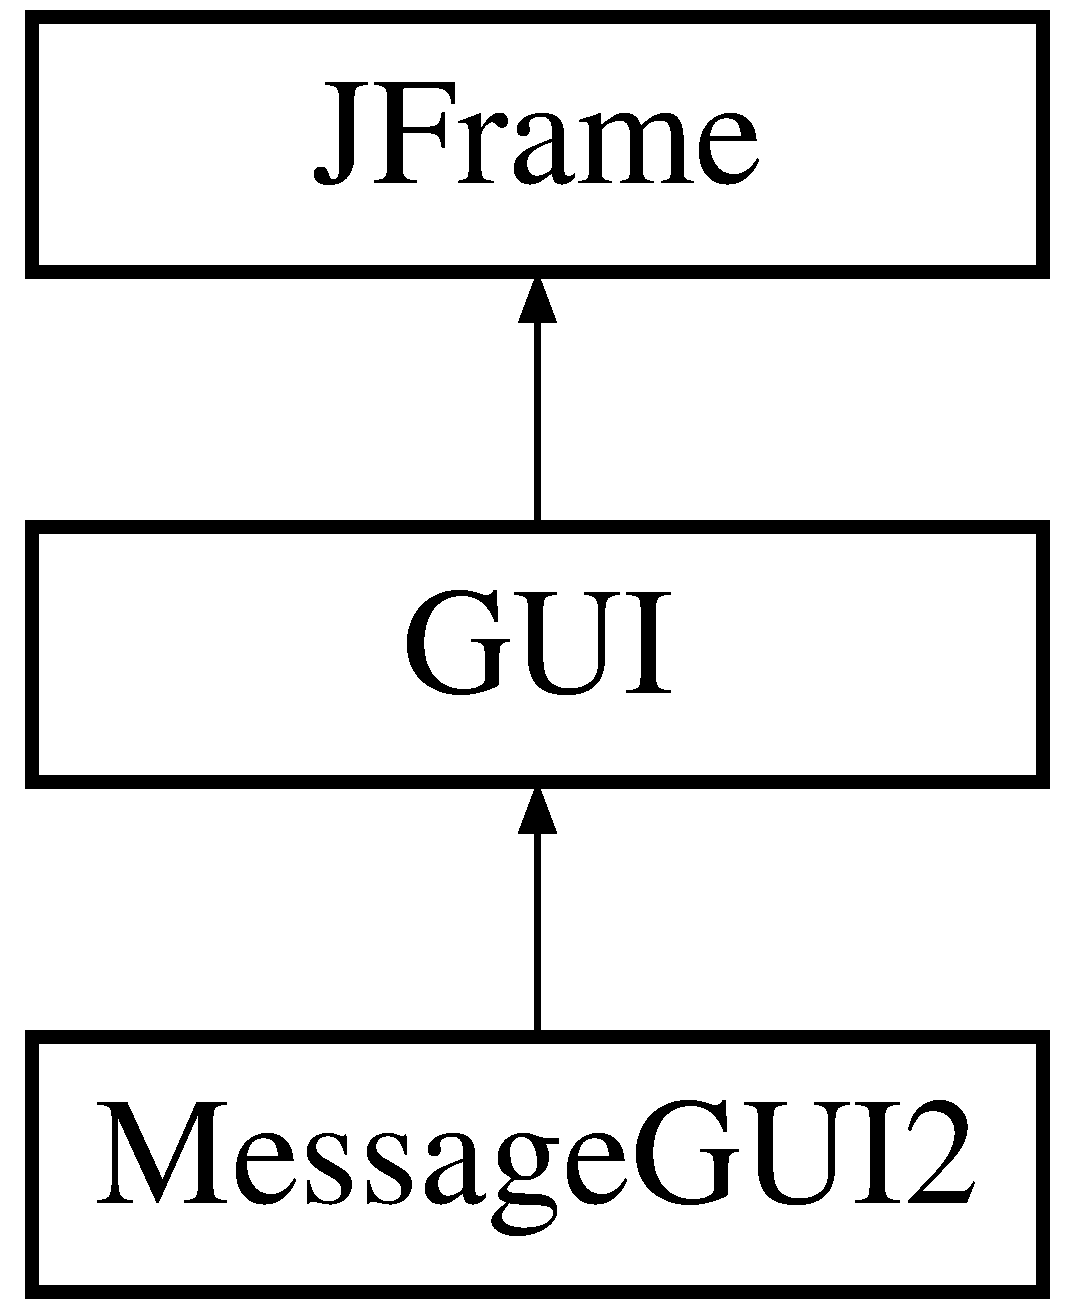
\includegraphics[height=3.000000cm]{class_message_g_u_i2}
\end{center}
\end{figure}
\subsection*{Public Member Functions}
\begin{DoxyCompactItemize}
\item 
\hyperlink{class_message_g_u_i2_a6cb5dea82c3d14b3bc925ee904219840}{Message\+G\+U\+I2} (\hyperlink{class_account}{Account} current\+\_\+user)  throws Exception
\begin{DoxyCompactList}\small\item\em Generates a list of friends that have started a conversation with the current user and displays the whole convo history as well as allows the user to send a text message back. \end{DoxyCompactList}\item 
String \hyperlink{class_message_g_u_i2_a3dfc57369fa2003712cebd9c2cf40fd1}{get\+\_\+content} (String sender, Array\+List$<$ \hyperlink{class_text_message}{Text\+Message} $>$ txt)
\end{DoxyCompactItemize}
\subsection*{Static Public Member Functions}
\begin{DoxyCompactItemize}
\item 
\mbox{\Hypertarget{class_message_g_u_i2_ad8fa5c5e6f8daa39a97eb69e7a575f97}\label{class_message_g_u_i2_ad8fa5c5e6f8daa39a97eb69e7a575f97}} 
static void \hyperlink{class_message_g_u_i2_ad8fa5c5e6f8daa39a97eb69e7a575f97}{main} (String\mbox{[}$\,$\mbox{]} args)  throws Exception
\begin{DoxyCompactList}\small\item\em Implemented for testing purposes. \end{DoxyCompactList}\end{DoxyCompactItemize}


\subsection{Constructor \& Destructor Documentation}
\mbox{\Hypertarget{class_message_g_u_i2_a6cb5dea82c3d14b3bc925ee904219840}\label{class_message_g_u_i2_a6cb5dea82c3d14b3bc925ee904219840}} 
\index{Message\+G\+U\+I2@{Message\+G\+U\+I2}!Message\+G\+U\+I2@{Message\+G\+U\+I2}}
\index{Message\+G\+U\+I2@{Message\+G\+U\+I2}!Message\+G\+U\+I2@{Message\+G\+U\+I2}}
\subsubsection{\texorpdfstring{Message\+G\+U\+I2()}{MessageGUI2()}}
{\footnotesize\ttfamily Message\+G\+U\+I2.\+Message\+G\+U\+I2 (\begin{DoxyParamCaption}\item[{\hyperlink{class_account}{Account}}]{current\+\_\+user }\end{DoxyParamCaption}) throws Exception}



Generates a list of friends that have started a conversation with the current user and displays the whole convo history as well as allows the user to send a text message back. 


\begin{DoxyParams}{Parameters}
{\em current\+\_\+user} & Reference to the logged in \hyperlink{class_account}{Account} \\
\hline
\end{DoxyParams}


\subsection{Member Function Documentation}
\mbox{\Hypertarget{class_message_g_u_i2_a3dfc57369fa2003712cebd9c2cf40fd1}\label{class_message_g_u_i2_a3dfc57369fa2003712cebd9c2cf40fd1}} 
\index{Message\+G\+U\+I2@{Message\+G\+U\+I2}!get\+\_\+content@{get\+\_\+content}}
\index{get\+\_\+content@{get\+\_\+content}!Message\+G\+U\+I2@{Message\+G\+U\+I2}}
\subsubsection{\texorpdfstring{get\+\_\+content()}{get\_content()}}
{\footnotesize\ttfamily String Message\+G\+U\+I2.\+get\+\_\+content (\begin{DoxyParamCaption}\item[{String}]{sender,  }\item[{Array\+List$<$ \hyperlink{class_text_message}{Text\+Message} $>$}]{txt }\end{DoxyParamCaption})}


\begin{DoxyParams}{Parameters}
{\em sender} & username of the sender \\
\hline
{\em txt} & Array\+List of messages to pull content from \\
\hline
\end{DoxyParams}
\begin{DoxyReturn}{Returns}
conversation history between current user and some sender 
\end{DoxyReturn}


The documentation for this class was generated from the following file\+:\begin{DoxyCompactItemize}
\item 
readwrite/Message\+G\+U\+I2.\+java\end{DoxyCompactItemize}

\hypertarget{class_profile_g_u_i}{}\section{Profile\+G\+UI Class Reference}
\label{class_profile_g_u_i}\index{Profile\+G\+UI@{Profile\+G\+UI}}
Inheritance diagram for Profile\+G\+UI\+:\begin{figure}[H]
\begin{center}
\leavevmode
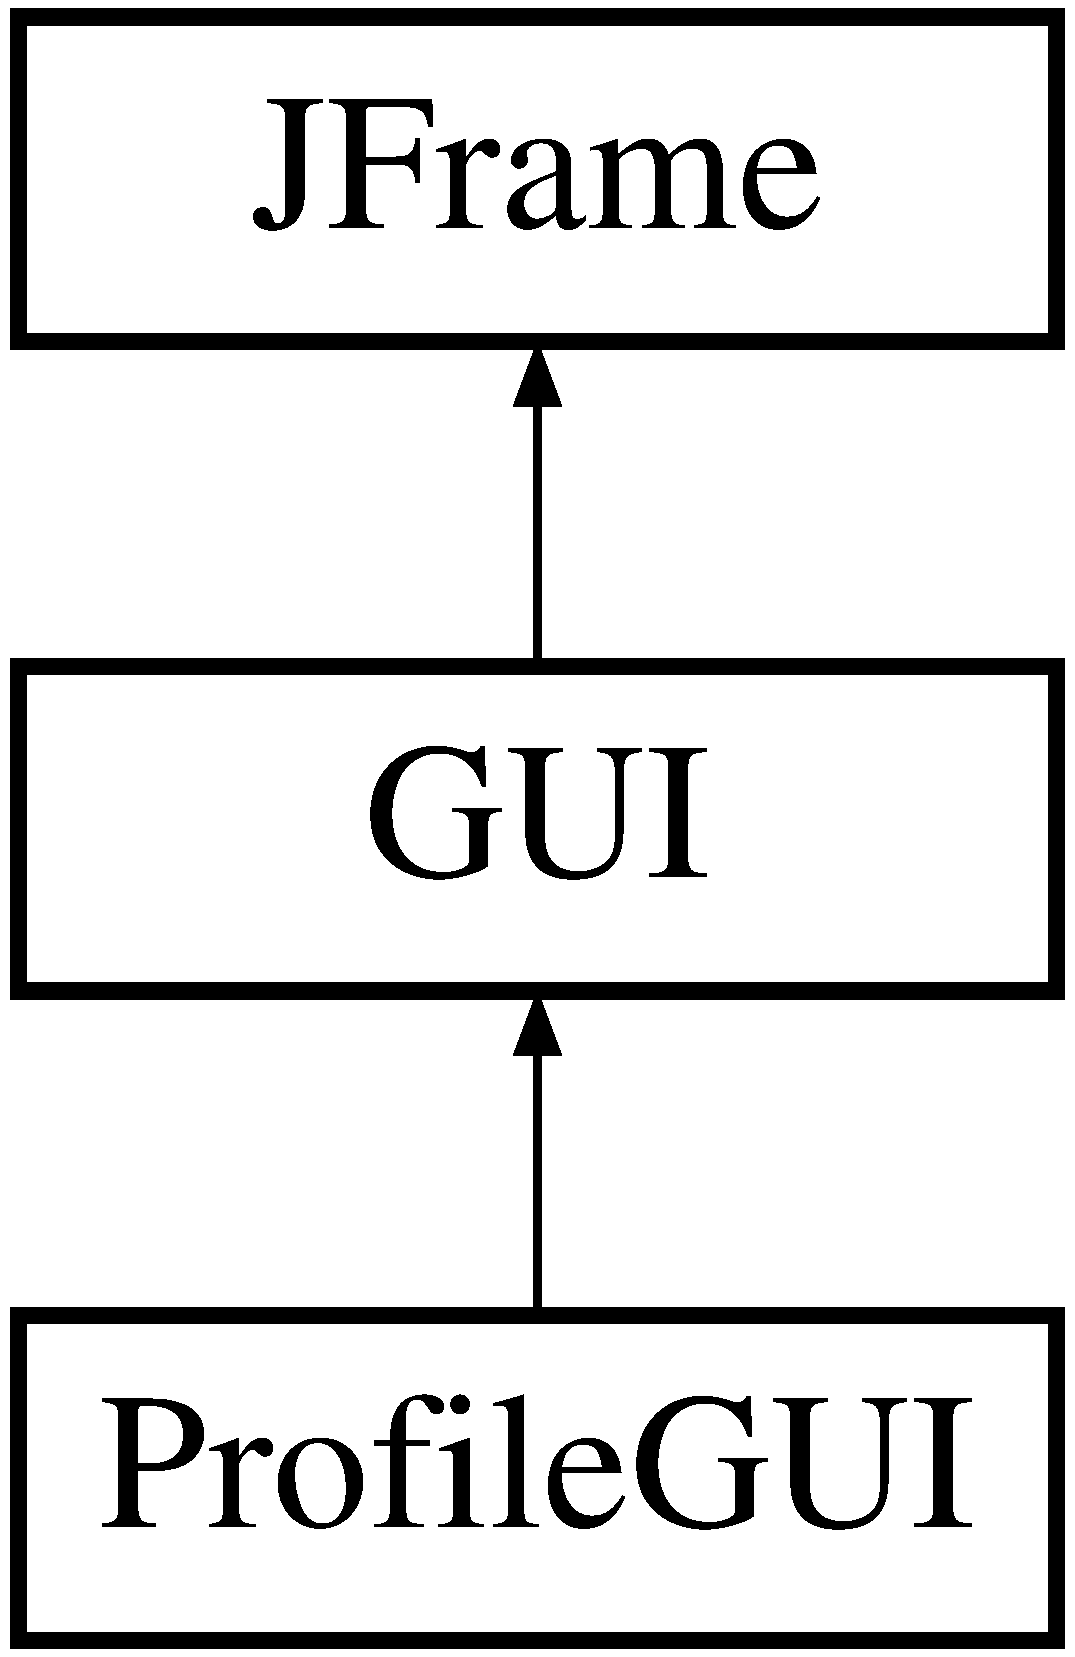
\includegraphics[height=3.000000cm]{class_profile_g_u_i}
\end{center}
\end{figure}
\subsection*{Public Member Functions}
\begin{DoxyCompactItemize}
\item 
\mbox{\Hypertarget{class_profile_g_u_i_ad1e8cf1893340cf951e96cbc5af36c1f}\label{class_profile_g_u_i_ad1e8cf1893340cf951e96cbc5af36c1f}} 
{\bfseries Profile\+G\+UI} (\hyperlink{class_account}{Account} acc)  throws Exception 
\item 
\mbox{\Hypertarget{class_profile_g_u_i_a440446d79e5c04a4734e5266d1dcdc04}\label{class_profile_g_u_i_a440446d79e5c04a4734e5266d1dcdc04}} 
void {\bfseries profilesetup} (\hyperlink{class_account}{Account} acc)  throws Exception
\end{DoxyCompactItemize}
\subsection*{Static Public Member Functions}
\begin{DoxyCompactItemize}
\item 
\mbox{\Hypertarget{class_profile_g_u_i_af56b9f8787202e794f33100ba8ed27df}\label{class_profile_g_u_i_af56b9f8787202e794f33100ba8ed27df}} 
static void {\bfseries main} (String\mbox{[}$\,$\mbox{]} args)  throws Exception 
\end{DoxyCompactItemize}


The documentation for this class was generated from the following file\+:\begin{DoxyCompactItemize}
\item 
readwrite/Profile\+G\+U\+I.\+java\end{DoxyCompactItemize}

\hypertarget{class_profile_image_panel}{}\section{Profile\+Image\+Panel Class Reference}
\label{class_profile_image_panel}\index{Profile\+Image\+Panel@{Profile\+Image\+Panel}}
Inheritance diagram for Profile\+Image\+Panel\+:\begin{figure}[H]
\begin{center}
\leavevmode
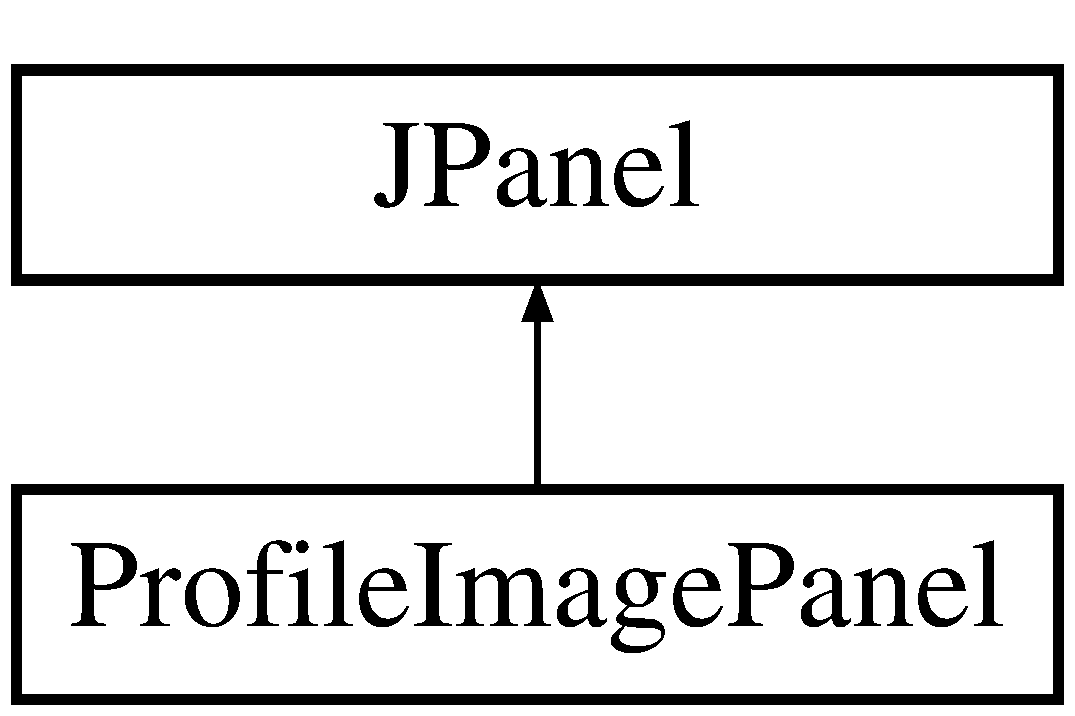
\includegraphics[height=2.000000cm]{class_profile_image_panel}
\end{center}
\end{figure}
\subsection*{Public Member Functions}
\begin{DoxyCompactItemize}
\item 
\hyperlink{class_profile_image_panel_a97acf7180ff6c375a9d310c0d09828db}{Profile\+Image\+Panel} (String filename)
\end{DoxyCompactItemize}
\subsection*{Protected Member Functions}
\begin{DoxyCompactItemize}
\item 
\mbox{\Hypertarget{class_profile_image_panel_ab1afa1f852a9f304d34c25a05f47f937}\label{class_profile_image_panel_ab1afa1f852a9f304d34c25a05f47f937}} 
void \hyperlink{class_profile_image_panel_ab1afa1f852a9f304d34c25a05f47f937}{paint\+Component} (Graphics g)
\begin{DoxyCompactList}\small\item\em Overwritten method to paint the image component on the panel. \end{DoxyCompactList}\end{DoxyCompactItemize}


\subsection{Constructor \& Destructor Documentation}
\mbox{\Hypertarget{class_profile_image_panel_a97acf7180ff6c375a9d310c0d09828db}\label{class_profile_image_panel_a97acf7180ff6c375a9d310c0d09828db}} 
\index{Profile\+Image\+Panel@{Profile\+Image\+Panel}!Profile\+Image\+Panel@{Profile\+Image\+Panel}}
\index{Profile\+Image\+Panel@{Profile\+Image\+Panel}!Profile\+Image\+Panel@{Profile\+Image\+Panel}}
\subsubsection{\texorpdfstring{Profile\+Image\+Panel()}{ProfileImagePanel()}}
{\footnotesize\ttfamily Profile\+Image\+Panel.\+Profile\+Image\+Panel (\begin{DoxyParamCaption}\item[{String}]{filename }\end{DoxyParamCaption})}


\begin{DoxyParams}{Parameters}
{\em filename} & The image you want displayed \\
\hline
\end{DoxyParams}


The documentation for this class was generated from the following file\+:\begin{DoxyCompactItemize}
\item 
readwrite/Profile\+Image\+Panel.\+java\end{DoxyCompactItemize}

\hypertarget{class_read_write_account}{}\section{Read\+Write\+Account Class Reference}
\label{class_read_write_account}\index{Read\+Write\+Account@{Read\+Write\+Account}}


Inherits Read\+Write$<$ E $>$.

\subsection*{Public Member Functions}
\begin{DoxyCompactItemize}
\item 
\hyperlink{class_read_write_account_a3c89be0e9259ae04b7b88de6d791f2ff}{Read\+Write\+Account} (String filename)  throws Exception     
\begin{DoxyCompactList}\small\item\em Setup a connection to the database and a way of querying it. \end{DoxyCompactList}\item 
Statement \hyperlink{class_read_write_account_aec86c1bc4029bb3699c85dee12982de8}{create\+\_\+account\+\_\+table} (Connection conn, Statement stmt)  throws Exception     
\begin{DoxyCompactList}\small\item\em Runs an S\+QL statement to generate a new table in the db. \end{DoxyCompactList}\item 
\hyperlink{class_account}{Account} \hyperlink{class_read_write_account_adb0ddd0ce6641f10c1b9220c670552e9}{read} (String query)  throws Exception     
\begin{DoxyCompactList}\small\item\em Runs a query by username on the database of accounts. \end{DoxyCompactList}\item 
Array\+List$<$ \hyperlink{class_account}{Account} $>$ \hyperlink{class_read_write_account_af566baef11164e567122f337ce3dc2cc}{read\+\_\+all\+\_\+accounts} ()  throws Exception     
\begin{DoxyCompactList}\small\item\em Get an Array\+List of every account in the table. \end{DoxyCompactList}\item 
int \hyperlink{class_read_write_account_afdac5d7a98c49a6daa71564116d3c49f}{read\+\_\+int\+\_\+column} (String query, String col)  throws Exception     
\begin{DoxyCompactList}\small\item\em Given a username, will return the specified col for that user but only if the column type is an int. \end{DoxyCompactList}\item 
String \hyperlink{class_read_write_account_a088ef942f68e5e969c153b241b534ff5}{read\+\_\+string\+\_\+column} (String query, String col)  throws Exception     
\begin{DoxyCompactList}\small\item\em Given a username, return the specified column for that user but only if the type of that column is a string (V\+A\+R\+C\+H\+AR in S\+QL) \end{DoxyCompactList}\item 
\mbox{\Hypertarget{class_read_write_account_a4cba2dcd68941a0685d952324e69b63e}\label{class_read_write_account_a4cba2dcd68941a0685d952324e69b63e}} 
void \hyperlink{class_read_write_account_a4cba2dcd68941a0685d952324e69b63e}{write} (\hyperlink{class_account}{Account} acc\+\_\+info)  throws Exception     
\begin{DoxyCompactList}\small\item\em acc\+\_\+info is an \hyperlink{class_account}{Account} object to store in the table \hyperlink{class_account}{Account} in that E\+X\+A\+CT order. \end{DoxyCompactList}\item 
\mbox{\Hypertarget{class_read_write_account_a3579e4d897bffab4b4406e18414f3835}\label{class_read_write_account_a3579e4d897bffab4b4406e18414f3835}} 
void \hyperlink{class_read_write_account_a3579e4d897bffab4b4406e18414f3835}{write\+\_\+new\+\_\+messages\+\_\+column} (String username, int val)  throws Exception     
\begin{DoxyCompactList}\small\item\em increment the new\+\_\+messages column by val for some username (could have made this a general int column updater but the only other int column is Account\+ID which will never be changed) (negative values work in order to reset a column) \end{DoxyCompactList}\item 
\mbox{\Hypertarget{class_read_write_account_a2a0ede48891400ae63ca99f600c6899c}\label{class_read_write_account_a2a0ede48891400ae63ca99f600c6899c}} 
void \hyperlink{class_read_write_account_a2a0ede48891400ae63ca99f600c6899c}{write\+\_\+string\+\_\+column} (String username, String col, String new\+\_\+val)  throws Exception     
\begin{DoxyCompactList}\small\item\em updates a given column with a given value for a given username (Prepared\+Statements dont allow column names to be passed so had to do it this way) \end{DoxyCompactList}\end{DoxyCompactItemize}
\subsection*{Static Public Member Functions}
\begin{DoxyCompactItemize}
\item 
\mbox{\Hypertarget{class_read_write_account_afb480d9aef80c5b153cf14e581a09fb2}\label{class_read_write_account_afb480d9aef80c5b153cf14e581a09fb2}} 
static void \hyperlink{class_read_write_account_afb480d9aef80c5b153cf14e581a09fb2}{main} (String\mbox{[}$\,$\mbox{]} args)  throws Exception     
\begin{DoxyCompactList}\small\item\em Only used for testing purposes. \end{DoxyCompactList}\end{DoxyCompactItemize}


\subsection{Constructor \& Destructor Documentation}
\mbox{\Hypertarget{class_read_write_account_a3c89be0e9259ae04b7b88de6d791f2ff}\label{class_read_write_account_a3c89be0e9259ae04b7b88de6d791f2ff}} 
\index{Read\+Write\+Account@{Read\+Write\+Account}!Read\+Write\+Account@{Read\+Write\+Account}}
\index{Read\+Write\+Account@{Read\+Write\+Account}!Read\+Write\+Account@{Read\+Write\+Account}}
\subsubsection{\texorpdfstring{Read\+Write\+Account()}{ReadWriteAccount()}}
{\footnotesize\ttfamily Read\+Write\+Account.\+Read\+Write\+Account (\begin{DoxyParamCaption}\item[{String}]{filename }\end{DoxyParamCaption}) throws Exception}



Setup a connection to the database and a way of querying it. 


\begin{DoxyParams}{Parameters}
{\em filename} & The database we want to use \\
\hline
\end{DoxyParams}


\subsection{Member Function Documentation}
\mbox{\Hypertarget{class_read_write_account_aec86c1bc4029bb3699c85dee12982de8}\label{class_read_write_account_aec86c1bc4029bb3699c85dee12982de8}} 
\index{Read\+Write\+Account@{Read\+Write\+Account}!create\+\_\+account\+\_\+table@{create\+\_\+account\+\_\+table}}
\index{create\+\_\+account\+\_\+table@{create\+\_\+account\+\_\+table}!Read\+Write\+Account@{Read\+Write\+Account}}
\subsubsection{\texorpdfstring{create\+\_\+account\+\_\+table()}{create\_account\_table()}}
{\footnotesize\ttfamily Statement Read\+Write\+Account.\+create\+\_\+account\+\_\+table (\begin{DoxyParamCaption}\item[{Connection}]{conn,  }\item[{Statement}]{stmt }\end{DoxyParamCaption}) throws Exception}



Runs an S\+QL statement to generate a new table in the db. 


\begin{DoxyParams}{Parameters}
{\em conn} & The connection object \\
\hline
{\em stmt} & A null pointing statement object \\
\hline
\end{DoxyParams}
\begin{DoxyReturn}{Returns}
The statement object connected to the db 
\end{DoxyReturn}
\mbox{\Hypertarget{class_read_write_account_adb0ddd0ce6641f10c1b9220c670552e9}\label{class_read_write_account_adb0ddd0ce6641f10c1b9220c670552e9}} 
\index{Read\+Write\+Account@{Read\+Write\+Account}!read@{read}}
\index{read@{read}!Read\+Write\+Account@{Read\+Write\+Account}}
\subsubsection{\texorpdfstring{read()}{read()}}
{\footnotesize\ttfamily \hyperlink{class_account}{Account} Read\+Write\+Account.\+read (\begin{DoxyParamCaption}\item[{String}]{query }\end{DoxyParamCaption}) throws Exception}



Runs a query by username on the database of accounts. 


\begin{DoxyParams}{Parameters}
{\em query} & Array\+List of one argument, the searched for username \\
\hline
\end{DoxyParams}
\begin{DoxyReturn}{Returns}
\hyperlink{class_account}{Account} object of the username searched for 
\end{DoxyReturn}
\mbox{\Hypertarget{class_read_write_account_af566baef11164e567122f337ce3dc2cc}\label{class_read_write_account_af566baef11164e567122f337ce3dc2cc}} 
\index{Read\+Write\+Account@{Read\+Write\+Account}!read\+\_\+all\+\_\+accounts@{read\+\_\+all\+\_\+accounts}}
\index{read\+\_\+all\+\_\+accounts@{read\+\_\+all\+\_\+accounts}!Read\+Write\+Account@{Read\+Write\+Account}}
\subsubsection{\texorpdfstring{read\+\_\+all\+\_\+accounts()}{read\_all\_accounts()}}
{\footnotesize\ttfamily Array\+List$<$\hyperlink{class_account}{Account}$>$ Read\+Write\+Account.\+read\+\_\+all\+\_\+accounts (\begin{DoxyParamCaption}{ }\end{DoxyParamCaption}) throws Exception}



Get an Array\+List of every account in the table. 

\begin{DoxyReturn}{Returns}
Array\+List of Accounts in the db 
\end{DoxyReturn}
\mbox{\Hypertarget{class_read_write_account_afdac5d7a98c49a6daa71564116d3c49f}\label{class_read_write_account_afdac5d7a98c49a6daa71564116d3c49f}} 
\index{Read\+Write\+Account@{Read\+Write\+Account}!read\+\_\+int\+\_\+column@{read\+\_\+int\+\_\+column}}
\index{read\+\_\+int\+\_\+column@{read\+\_\+int\+\_\+column}!Read\+Write\+Account@{Read\+Write\+Account}}
\subsubsection{\texorpdfstring{read\+\_\+int\+\_\+column()}{read\_int\_column()}}
{\footnotesize\ttfamily int Read\+Write\+Account.\+read\+\_\+int\+\_\+column (\begin{DoxyParamCaption}\item[{String}]{query,  }\item[{String}]{col }\end{DoxyParamCaption}) throws Exception}



Given a username, will return the specified col for that user but only if the column type is an int. 

You can get the following columns\+: Account\+ID \& new\+\_\+messages \mbox{\Hypertarget{class_read_write_account_a088ef942f68e5e969c153b241b534ff5}\label{class_read_write_account_a088ef942f68e5e969c153b241b534ff5}} 
\index{Read\+Write\+Account@{Read\+Write\+Account}!read\+\_\+string\+\_\+column@{read\+\_\+string\+\_\+column}}
\index{read\+\_\+string\+\_\+column@{read\+\_\+string\+\_\+column}!Read\+Write\+Account@{Read\+Write\+Account}}
\subsubsection{\texorpdfstring{read\+\_\+string\+\_\+column()}{read\_string\_column()}}
{\footnotesize\ttfamily String Read\+Write\+Account.\+read\+\_\+string\+\_\+column (\begin{DoxyParamCaption}\item[{String}]{query,  }\item[{String}]{col }\end{DoxyParamCaption}) throws Exception}



Given a username, return the specified column for that user but only if the type of that column is a string (V\+A\+R\+C\+H\+AR in S\+QL) 

You can get the following columns\+: username, first\+\_\+name, surname, mob\+\_\+num, dob, city, prev\+\_\+session, profile\+\_\+img 

The documentation for this class was generated from the following file\+:\begin{DoxyCompactItemize}
\item 
readwrite/Read\+Write\+Account.\+java\end{DoxyCompactItemize}

\hypertarget{class_read_write_friends}{}\section{Read\+Write\+Friends Class Reference}
\label{class_read_write_friends}\index{Read\+Write\+Friends@{Read\+Write\+Friends}}


Inherits Read\+Write$<$ E $>$.

\subsection*{Public Member Functions}
\begin{DoxyCompactItemize}
\item 
\hyperlink{class_read_write_friends_afccd5d07c3f694a74617a749ee4d5d09}{Read\+Write\+Friends} (String filename)  throws Exception     
\begin{DoxyCompactList}\small\item\em Sets up a connection to the db. \end{DoxyCompactList}\item 
Statement \hyperlink{class_read_write_friends_abd8ff6b1154e07ae729ce151d7160fa9}{create\+\_\+friends\+\_\+table} (Connection conn, Statement stmt)  throws Exception     
\begin{DoxyCompactList}\small\item\em Runs an S\+QL statement to create the Friends table. \end{DoxyCompactList}\item 
\mbox{\Hypertarget{class_read_write_friends_a1a30e3f1adc90e7e69c3c4855dc00738}\label{class_read_write_friends_a1a30e3f1adc90e7e69c3c4855dc00738}} 
Array\+List$<$ \hyperlink{class_account}{Account} $>$ \hyperlink{class_read_write_friends_a1a30e3f1adc90e7e69c3c4855dc00738}{read} (String query)  throws Exception     
\begin{DoxyCompactList}\small\item\em unused method \end{DoxyCompactList}\item 
Array\+List$<$ \hyperlink{class_account}{Account} $>$ \hyperlink{class_read_write_friends_a1ca7ef459d275d7de8274ce119e4895d}{get\+\_\+all\+\_\+friends} ()  throws Exception     
\item 
Array\+List$<$ \hyperlink{class_account}{Account} $>$ \hyperlink{class_read_write_friends_ab55c8c1b2fc693bad5da1da3774dfab2}{get\+\_\+all\+\_\+requests} (\hyperlink{class_account}{Account} acc)  throws Exception     
\begin{DoxyCompactList}\small\item\em Given some account, computes all friend requests they\textquotesingle{}ll have recieved. \end{DoxyCompactList}\item 
\hyperlink{class_account}{Account} \hyperlink{class_read_write_friends_a56f74832f8bc0bee6c7d48aad84878eb}{get\+\_\+account\+\_\+from\+\_\+id} (int acc\+\_\+id)  throws Exception     
\begin{DoxyCompactList}\small\item\em Given an Account\+ID, pull information from the database and generate an account object. \end{DoxyCompactList}\item 
void \hyperlink{class_read_write_friends_ae754f5aa3e65cde59ad619a56f7b318e}{write} (Array\+List$<$ \hyperlink{class_account}{Account} $>$ to\+\_\+add)  throws Exception     
\begin{DoxyCompactList}\small\item\em to\+\_\+add will contain\+: \mbox{[}Account1, Account2\mbox{]} where both are \hyperlink{class_account}{Account} objects \end{DoxyCompactList}\item 
int \hyperlink{class_read_write_friends_abbe5f06f2119c20d3015b91b4b1c728f}{check\+\_\+friends\+\_\+status} (\hyperlink{class_account}{Account} a1, \hyperlink{class_account}{Account} a2)  throws Exception     
\begin{DoxyCompactList}\small\item\em Determines if 2 accounts have a pending or accepted friendship relation. \end{DoxyCompactList}\item 
\mbox{\Hypertarget{class_read_write_friends_aee917f985979bdf89bb55b84cb52017c}\label{class_read_write_friends_aee917f985979bdf89bb55b84cb52017c}} 
int \hyperlink{class_read_write_friends_aee917f985979bdf89bb55b84cb52017c}{get\+\_\+acc\+\_\+id} (\hyperlink{class_account}{Account} acc)  throws Exception     
\begin{DoxyCompactList}\small\item\em Get information about an account given the desired column and the relevent \hyperlink{class_account}{Account} object. \end{DoxyCompactList}\end{DoxyCompactItemize}
\subsection*{Static Public Member Functions}
\begin{DoxyCompactItemize}
\item 
\mbox{\Hypertarget{class_read_write_friends_ac2039776a76fdbdc416cfa3cd16495e6}\label{class_read_write_friends_ac2039776a76fdbdc416cfa3cd16495e6}} 
static void \hyperlink{class_read_write_friends_ac2039776a76fdbdc416cfa3cd16495e6}{main} (String\mbox{[}$\,$\mbox{]} args)  throws Exception     
\begin{DoxyCompactList}\small\item\em Testing for \hyperlink{class_read_write_friends}{Read\+Write\+Friends} functionality. \end{DoxyCompactList}\end{DoxyCompactItemize}


\subsection{Constructor \& Destructor Documentation}
\mbox{\Hypertarget{class_read_write_friends_afccd5d07c3f694a74617a749ee4d5d09}\label{class_read_write_friends_afccd5d07c3f694a74617a749ee4d5d09}} 
\index{Read\+Write\+Friends@{Read\+Write\+Friends}!Read\+Write\+Friends@{Read\+Write\+Friends}}
\index{Read\+Write\+Friends@{Read\+Write\+Friends}!Read\+Write\+Friends@{Read\+Write\+Friends}}
\subsubsection{\texorpdfstring{Read\+Write\+Friends()}{ReadWriteFriends()}}
{\footnotesize\ttfamily Read\+Write\+Friends.\+Read\+Write\+Friends (\begin{DoxyParamCaption}\item[{String}]{filename }\end{DoxyParamCaption}) throws Exception}



Sets up a connection to the db. 


\begin{DoxyParams}{Parameters}
{\em filename} & The db we want to use \\
\hline
\end{DoxyParams}


\subsection{Member Function Documentation}
\mbox{\Hypertarget{class_read_write_friends_abbe5f06f2119c20d3015b91b4b1c728f}\label{class_read_write_friends_abbe5f06f2119c20d3015b91b4b1c728f}} 
\index{Read\+Write\+Friends@{Read\+Write\+Friends}!check\+\_\+friends\+\_\+status@{check\+\_\+friends\+\_\+status}}
\index{check\+\_\+friends\+\_\+status@{check\+\_\+friends\+\_\+status}!Read\+Write\+Friends@{Read\+Write\+Friends}}
\subsubsection{\texorpdfstring{check\+\_\+friends\+\_\+status()}{check\_friends\_status()}}
{\footnotesize\ttfamily int Read\+Write\+Friends.\+check\+\_\+friends\+\_\+status (\begin{DoxyParamCaption}\item[{\hyperlink{class_account}{Account}}]{a1,  }\item[{\hyperlink{class_account}{Account}}]{a2 }\end{DoxyParamCaption}) throws Exception}



Determines if 2 accounts have a pending or accepted friendship relation. 

if 1 is returned then friendship is P\+E\+N\+D\+I\+NG if 2 is returned then friendship is A\+C\+C\+E\+P\+T\+ED \mbox{\Hypertarget{class_read_write_friends_abd8ff6b1154e07ae729ce151d7160fa9}\label{class_read_write_friends_abd8ff6b1154e07ae729ce151d7160fa9}} 
\index{Read\+Write\+Friends@{Read\+Write\+Friends}!create\+\_\+friends\+\_\+table@{create\+\_\+friends\+\_\+table}}
\index{create\+\_\+friends\+\_\+table@{create\+\_\+friends\+\_\+table}!Read\+Write\+Friends@{Read\+Write\+Friends}}
\subsubsection{\texorpdfstring{create\+\_\+friends\+\_\+table()}{create\_friends\_table()}}
{\footnotesize\ttfamily Statement Read\+Write\+Friends.\+create\+\_\+friends\+\_\+table (\begin{DoxyParamCaption}\item[{Connection}]{conn,  }\item[{Statement}]{stmt }\end{DoxyParamCaption}) throws Exception}



Runs an S\+QL statement to create the Friends table. 


\begin{DoxyParams}{Parameters}
{\em conn} & The connection object to the db \\
\hline
{\em stmt} & Null pointing statement to be set up \\
\hline
\end{DoxyParams}
\begin{DoxyReturn}{Returns}
the setup statement object 
\end{DoxyReturn}
\mbox{\Hypertarget{class_read_write_friends_a56f74832f8bc0bee6c7d48aad84878eb}\label{class_read_write_friends_a56f74832f8bc0bee6c7d48aad84878eb}} 
\index{Read\+Write\+Friends@{Read\+Write\+Friends}!get\+\_\+account\+\_\+from\+\_\+id@{get\+\_\+account\+\_\+from\+\_\+id}}
\index{get\+\_\+account\+\_\+from\+\_\+id@{get\+\_\+account\+\_\+from\+\_\+id}!Read\+Write\+Friends@{Read\+Write\+Friends}}
\subsubsection{\texorpdfstring{get\+\_\+account\+\_\+from\+\_\+id()}{get\_account\_from\_id()}}
{\footnotesize\ttfamily \hyperlink{class_account}{Account} Read\+Write\+Friends.\+get\+\_\+account\+\_\+from\+\_\+id (\begin{DoxyParamCaption}\item[{int}]{acc\+\_\+id }\end{DoxyParamCaption}) throws Exception}



Given an Account\+ID, pull information from the database and generate an account object. 


\begin{DoxyParams}{Parameters}
{\em acc\+\_\+id} & The Account\+ID we\textquotesingle{}re using \\
\hline
\end{DoxyParams}
\begin{DoxyReturn}{Returns}
The account we want 
\end{DoxyReturn}
\mbox{\Hypertarget{class_read_write_friends_a1ca7ef459d275d7de8274ce119e4895d}\label{class_read_write_friends_a1ca7ef459d275d7de8274ce119e4895d}} 
\index{Read\+Write\+Friends@{Read\+Write\+Friends}!get\+\_\+all\+\_\+friends@{get\+\_\+all\+\_\+friends}}
\index{get\+\_\+all\+\_\+friends@{get\+\_\+all\+\_\+friends}!Read\+Write\+Friends@{Read\+Write\+Friends}}
\subsubsection{\texorpdfstring{get\+\_\+all\+\_\+friends()}{get\_all\_friends()}}
{\footnotesize\ttfamily Array\+List$<$\hyperlink{class_account}{Account}$>$ Read\+Write\+Friends.\+get\+\_\+all\+\_\+friends (\begin{DoxyParamCaption}{ }\end{DoxyParamCaption}) throws Exception}


\begin{DoxyItemize}
\item get a table of all friendships stored in the database
\item return list of account objects where\+: \mbox{[}acc1, acc2, acc1, acc5, acc3, acc6\mbox{]} means \+: acc1 and acc2 are F\+R\+I\+E\+N\+DS \+: acc1 and acc5 are F\+R\+I\+E\+N\+DS \+: acc3 and acc6 are F\+R\+I\+E\+N\+DS 
\end{DoxyItemize}\mbox{\Hypertarget{class_read_write_friends_ab55c8c1b2fc693bad5da1da3774dfab2}\label{class_read_write_friends_ab55c8c1b2fc693bad5da1da3774dfab2}} 
\index{Read\+Write\+Friends@{Read\+Write\+Friends}!get\+\_\+all\+\_\+requests@{get\+\_\+all\+\_\+requests}}
\index{get\+\_\+all\+\_\+requests@{get\+\_\+all\+\_\+requests}!Read\+Write\+Friends@{Read\+Write\+Friends}}
\subsubsection{\texorpdfstring{get\+\_\+all\+\_\+requests()}{get\_all\_requests()}}
{\footnotesize\ttfamily Array\+List$<$\hyperlink{class_account}{Account}$>$ Read\+Write\+Friends.\+get\+\_\+all\+\_\+requests (\begin{DoxyParamCaption}\item[{\hyperlink{class_account}{Account}}]{acc }\end{DoxyParamCaption}) throws Exception}



Given some account, computes all friend requests they\textquotesingle{}ll have recieved. 


\begin{DoxyParams}{Parameters}
{\em acc} & The account we\textquotesingle{}re checking \\
\hline
\end{DoxyParams}
\begin{DoxyReturn}{Returns}
Array\+List of all pending friend requests for some \hyperlink{class_account}{Account} 
\end{DoxyReturn}
\mbox{\Hypertarget{class_read_write_friends_ae754f5aa3e65cde59ad619a56f7b318e}\label{class_read_write_friends_ae754f5aa3e65cde59ad619a56f7b318e}} 
\index{Read\+Write\+Friends@{Read\+Write\+Friends}!write@{write}}
\index{write@{write}!Read\+Write\+Friends@{Read\+Write\+Friends}}
\subsubsection{\texorpdfstring{write()}{write()}}
{\footnotesize\ttfamily void Read\+Write\+Friends.\+write (\begin{DoxyParamCaption}\item[{Array\+List$<$ \hyperlink{class_account}{Account} $>$}]{to\+\_\+add }\end{DoxyParamCaption}) throws Exception}



to\+\_\+add will contain\+: \mbox{[}Account1, Account2\mbox{]} where both are \hyperlink{class_account}{Account} objects 

inserts a record for two accounts into the database checks if it\textquotesingle{}s a request or an acceptance notifys/updates accordingally 

The documentation for this class was generated from the following file\+:\begin{DoxyCompactItemize}
\item 
readwrite/Read\+Write\+Friends.\+java\end{DoxyCompactItemize}

\hypertarget{class_read_write_message}{}\section{Read\+Write\+Message Class Reference}
\label{class_read_write_message}\index{Read\+Write\+Message@{Read\+Write\+Message}}


Inherits Read\+Write$<$ E $>$.

\subsection*{Public Member Functions}
\begin{DoxyCompactItemize}
\item 
\hyperlink{class_read_write_message_a91757d43631c332753ef62b61e48413e}{Read\+Write\+Message} (String dbname, String filename)  throws Exception     
\begin{DoxyCompactList}\small\item\em Sets a connection up to the db and messages.\+txt. \end{DoxyCompactList}\item 
Array\+List$<$ \hyperlink{class_message}{Message} $>$ \hyperlink{class_read_write_message_a134117f3846976650506f858cd049059}{read} (String username)  throws Exception     
\begin{DoxyCompactList}\small\item\em given a username, it returns their entire message history \end{DoxyCompactList}\item 
\mbox{\Hypertarget{class_read_write_message_a28d03d35c19dfd67eb2b7ad7fd5ca414}\label{class_read_write_message_a28d03d35c19dfd67eb2b7ad7fd5ca414}} 
Array\+List$<$ \hyperlink{class_text_message}{Text\+Message} $>$ \hyperlink{class_read_write_message_a28d03d35c19dfd67eb2b7ad7fd5ca414}{read\+\_\+text\+\_\+messages} (String username)
\begin{DoxyCompactList}\small\item\em Gets all Text\+Messages recieved by a user. \end{DoxyCompactList}\item 
\mbox{\Hypertarget{class_read_write_message_a851db30870febb26793696aea0be156b}\label{class_read_write_message_a851db30870febb26793696aea0be156b}} 
Array\+List$<$ \hyperlink{class_u_r_l_message}{U\+R\+L\+Message} $>$ \hyperlink{class_read_write_message_a851db30870febb26793696aea0be156b}{read\+\_\+url\+\_\+messages} (String username)
\begin{DoxyCompactList}\small\item\em Gets all U\+R\+L\+Messages recieved by a user. \end{DoxyCompactList}\item 
\mbox{\Hypertarget{class_read_write_message_ae9e2f4265707803c35efce4defefbb07}\label{class_read_write_message_ae9e2f4265707803c35efce4defefbb07}} 
Array\+List$<$ \hyperlink{class_file_message}{File\+Message} $>$ \hyperlink{class_read_write_message_ae9e2f4265707803c35efce4defefbb07}{read\+\_\+file\+\_\+messages} (String username)
\begin{DoxyCompactList}\small\item\em Gets all File\+Messages recieved by a user. \end{DoxyCompactList}\item 
\mbox{\Hypertarget{class_read_write_message_ad9460192c9102b15579d7920ae5607bd}\label{class_read_write_message_ad9460192c9102b15579d7920ae5607bd}} 
void {\bfseries write} (Array\+List$<$ \hyperlink{class_message}{Message} $>$ msgs)  throws Exception     
\item 
\mbox{\Hypertarget{class_read_write_message_a754e9e7cd1cc2bc011147798fbf79d89}\label{class_read_write_message_a754e9e7cd1cc2bc011147798fbf79d89}} 
void \hyperlink{class_read_write_message_a754e9e7cd1cc2bc011147798fbf79d89}{write\+\_\+text\+\_\+message} (\hyperlink{class_text_message}{Text\+Message} m)  throws Exception     
\begin{DoxyCompactList}\small\item\em save a text message in messages.\+txt \end{DoxyCompactList}\item 
\mbox{\Hypertarget{class_read_write_message_ac705a1a4c26df2286f312d44363d2cc6}\label{class_read_write_message_ac705a1a4c26df2286f312d44363d2cc6}} 
void \hyperlink{class_read_write_message_ac705a1a4c26df2286f312d44363d2cc6}{write\+\_\+url\+\_\+message} (\hyperlink{class_u_r_l_message}{U\+R\+L\+Message} u)  throws Exception     
\begin{DoxyCompactList}\small\item\em Stores a \hyperlink{class_u_r_l_message}{U\+R\+L\+Message} object as a string in \textquotesingle{}messages.\+txt\textquotesingle{}. \end{DoxyCompactList}\item 
void \hyperlink{class_read_write_message_abea280f7f2a29c1edac9a4b9998972ed}{write\+\_\+file\+\_\+message} (\hyperlink{class_file_message}{File\+Message} f)  throws Exception     
\begin{DoxyCompactList}\small\item\em Stores a \hyperlink{class_file_message}{File\+Message} object as a string in \textquotesingle{}messages.\+txt\textquotesingle{} (file messages work as long as the file is in the files folder) \end{DoxyCompactList}\item 
void \hyperlink{class_read_write_message_a2a509bda22a84d2b46949c71984d205c}{write\+\_\+multi\+\_\+text\+\_\+msg} (Array\+List$<$ String $>$ recipients, \hyperlink{class_text_message}{Text\+Message} msg)  throws Exception     
\begin{DoxyCompactList}\small\item\em Sends a \hyperlink{class_text_message}{Text\+Message} object to a list of recipients. \end{DoxyCompactList}\item 
void \hyperlink{class_read_write_message_a9a005ffe1f6fd45a7490890e199731d5}{write\+\_\+multi\+\_\+url\+\_\+message} (Array\+List$<$ String $>$ recipients, \hyperlink{class_u_r_l_message}{U\+R\+L\+Message} msg)  throws Exception     
\begin{DoxyCompactList}\small\item\em Sends a \hyperlink{class_u_r_l_message}{U\+R\+L\+Message} object to a list of recipients. \end{DoxyCompactList}\item 
void \hyperlink{class_read_write_message_a8d406199a35776861428f76038aa5dc4}{write\+\_\+multi\+\_\+file\+\_\+message} (Array\+List$<$ String $>$ recipients, \hyperlink{class_file_message}{File\+Message} msg)  throws Exception     
\begin{DoxyCompactList}\small\item\em Sends a \hyperlink{class_file_message}{File\+Message} object to a list of recipients. \end{DoxyCompactList}\item 
void \hyperlink{class_read_write_message_ab95207fb27ef92136d39b454e7826fc5}{inc\+\_\+nm\+\_\+value} (String username)  throws Exception     
\begin{DoxyCompactList}\small\item\em Increments the new\+\_\+messages value of a user by 1. \end{DoxyCompactList}\item 
void \hyperlink{class_read_write_message_a92a8e0f94a1b67491af6a7fbfdb52501}{dec\+\_\+nm\+\_\+value} (String username)  throws Exception     
\begin{DoxyCompactList}\small\item\em Decrements the new\+\_\+messages value of a user by 1. \end{DoxyCompactList}\end{DoxyCompactItemize}
\subsection*{Static Public Member Functions}
\begin{DoxyCompactItemize}
\item 
\mbox{\Hypertarget{class_read_write_message_acbdb2486cf01f98e0288cedcf4747de9}\label{class_read_write_message_acbdb2486cf01f98e0288cedcf4747de9}} 
static void \hyperlink{class_read_write_message_acbdb2486cf01f98e0288cedcf4747de9}{main} (String\mbox{[}$\,$\mbox{]} args)  throws Exception     
\begin{DoxyCompactList}\small\item\em Implemented for testing purposes. \end{DoxyCompactList}\end{DoxyCompactItemize}


\subsection{Constructor \& Destructor Documentation}
\mbox{\Hypertarget{class_read_write_message_a91757d43631c332753ef62b61e48413e}\label{class_read_write_message_a91757d43631c332753ef62b61e48413e}} 
\index{Read\+Write\+Message@{Read\+Write\+Message}!Read\+Write\+Message@{Read\+Write\+Message}}
\index{Read\+Write\+Message@{Read\+Write\+Message}!Read\+Write\+Message@{Read\+Write\+Message}}
\subsubsection{\texorpdfstring{Read\+Write\+Message()}{ReadWriteMessage()}}
{\footnotesize\ttfamily Read\+Write\+Message.\+Read\+Write\+Message (\begin{DoxyParamCaption}\item[{String}]{dbname,  }\item[{String}]{filename }\end{DoxyParamCaption}) throws Exception}



Sets a connection up to the db and messages.\+txt. 


\begin{DoxyParams}{Parameters}
{\em dbname} & the db \\
\hline
{\em filename} & the message file \\
\hline
\end{DoxyParams}


\subsection{Member Function Documentation}
\mbox{\Hypertarget{class_read_write_message_a92a8e0f94a1b67491af6a7fbfdb52501}\label{class_read_write_message_a92a8e0f94a1b67491af6a7fbfdb52501}} 
\index{Read\+Write\+Message@{Read\+Write\+Message}!dec\+\_\+nm\+\_\+value@{dec\+\_\+nm\+\_\+value}}
\index{dec\+\_\+nm\+\_\+value@{dec\+\_\+nm\+\_\+value}!Read\+Write\+Message@{Read\+Write\+Message}}
\subsubsection{\texorpdfstring{dec\+\_\+nm\+\_\+value()}{dec\_nm\_value()}}
{\footnotesize\ttfamily void Read\+Write\+Message.\+dec\+\_\+nm\+\_\+value (\begin{DoxyParamCaption}\item[{String}]{username }\end{DoxyParamCaption}) throws Exception}



Decrements the new\+\_\+messages value of a user by 1. 


\begin{DoxyParams}{Parameters}
{\em username} & The account we\textquotesingle{}re editing \\
\hline
\end{DoxyParams}
\mbox{\Hypertarget{class_read_write_message_ab95207fb27ef92136d39b454e7826fc5}\label{class_read_write_message_ab95207fb27ef92136d39b454e7826fc5}} 
\index{Read\+Write\+Message@{Read\+Write\+Message}!inc\+\_\+nm\+\_\+value@{inc\+\_\+nm\+\_\+value}}
\index{inc\+\_\+nm\+\_\+value@{inc\+\_\+nm\+\_\+value}!Read\+Write\+Message@{Read\+Write\+Message}}
\subsubsection{\texorpdfstring{inc\+\_\+nm\+\_\+value()}{inc\_nm\_value()}}
{\footnotesize\ttfamily void Read\+Write\+Message.\+inc\+\_\+nm\+\_\+value (\begin{DoxyParamCaption}\item[{String}]{username }\end{DoxyParamCaption}) throws Exception}



Increments the new\+\_\+messages value of a user by 1. 


\begin{DoxyParams}{Parameters}
{\em username} & The account we\textquotesingle{}re editing \\
\hline
\end{DoxyParams}
\mbox{\Hypertarget{class_read_write_message_a134117f3846976650506f858cd049059}\label{class_read_write_message_a134117f3846976650506f858cd049059}} 
\index{Read\+Write\+Message@{Read\+Write\+Message}!read@{read}}
\index{read@{read}!Read\+Write\+Message@{Read\+Write\+Message}}
\subsubsection{\texorpdfstring{read()}{read()}}
{\footnotesize\ttfamily Array\+List$<$\hyperlink{class_message}{Message}$>$ Read\+Write\+Message.\+read (\begin{DoxyParamCaption}\item[{String}]{username }\end{DoxyParamCaption}) throws Exception}



given a username, it returns their entire message history 


\begin{DoxyParams}{Parameters}
{\em username} & The user \\
\hline
\end{DoxyParams}
\begin{DoxyReturn}{Returns}
an Array\+List of Messages 
\end{DoxyReturn}
\mbox{\Hypertarget{class_read_write_message_abea280f7f2a29c1edac9a4b9998972ed}\label{class_read_write_message_abea280f7f2a29c1edac9a4b9998972ed}} 
\index{Read\+Write\+Message@{Read\+Write\+Message}!write\+\_\+file\+\_\+message@{write\+\_\+file\+\_\+message}}
\index{write\+\_\+file\+\_\+message@{write\+\_\+file\+\_\+message}!Read\+Write\+Message@{Read\+Write\+Message}}
\subsubsection{\texorpdfstring{write\+\_\+file\+\_\+message()}{write\_file\_message()}}
{\footnotesize\ttfamily void Read\+Write\+Message.\+write\+\_\+file\+\_\+message (\begin{DoxyParamCaption}\item[{\hyperlink{class_file_message}{File\+Message}}]{f }\end{DoxyParamCaption}) throws Exception}



Stores a \hyperlink{class_file_message}{File\+Message} object as a string in \textquotesingle{}messages.\+txt\textquotesingle{} (file messages work as long as the file is in the files folder) 


\begin{DoxyParams}{Parameters}
{\em f} & The \hyperlink{class_file_message}{File\+Message} object \\
\hline
\end{DoxyParams}
\mbox{\Hypertarget{class_read_write_message_a8d406199a35776861428f76038aa5dc4}\label{class_read_write_message_a8d406199a35776861428f76038aa5dc4}} 
\index{Read\+Write\+Message@{Read\+Write\+Message}!write\+\_\+multi\+\_\+file\+\_\+message@{write\+\_\+multi\+\_\+file\+\_\+message}}
\index{write\+\_\+multi\+\_\+file\+\_\+message@{write\+\_\+multi\+\_\+file\+\_\+message}!Read\+Write\+Message@{Read\+Write\+Message}}
\subsubsection{\texorpdfstring{write\+\_\+multi\+\_\+file\+\_\+message()}{write\_multi\_file\_message()}}
{\footnotesize\ttfamily void Read\+Write\+Message.\+write\+\_\+multi\+\_\+file\+\_\+message (\begin{DoxyParamCaption}\item[{Array\+List$<$ String $>$}]{recipients,  }\item[{\hyperlink{class_file_message}{File\+Message}}]{msg }\end{DoxyParamCaption}) throws Exception}



Sends a \hyperlink{class_file_message}{File\+Message} object to a list of recipients. 


\begin{DoxyParams}{Parameters}
{\em recipients} & Array\+List of usernames \\
\hline
{\em msg} & The \hyperlink{class_file_message}{File\+Message} object \\
\hline
\end{DoxyParams}
\mbox{\Hypertarget{class_read_write_message_a2a509bda22a84d2b46949c71984d205c}\label{class_read_write_message_a2a509bda22a84d2b46949c71984d205c}} 
\index{Read\+Write\+Message@{Read\+Write\+Message}!write\+\_\+multi\+\_\+text\+\_\+msg@{write\+\_\+multi\+\_\+text\+\_\+msg}}
\index{write\+\_\+multi\+\_\+text\+\_\+msg@{write\+\_\+multi\+\_\+text\+\_\+msg}!Read\+Write\+Message@{Read\+Write\+Message}}
\subsubsection{\texorpdfstring{write\+\_\+multi\+\_\+text\+\_\+msg()}{write\_multi\_text\_msg()}}
{\footnotesize\ttfamily void Read\+Write\+Message.\+write\+\_\+multi\+\_\+text\+\_\+msg (\begin{DoxyParamCaption}\item[{Array\+List$<$ String $>$}]{recipients,  }\item[{\hyperlink{class_text_message}{Text\+Message}}]{msg }\end{DoxyParamCaption}) throws Exception}



Sends a \hyperlink{class_text_message}{Text\+Message} object to a list of recipients. 


\begin{DoxyParams}{Parameters}
{\em recipients} & Array\+List of usernames \\
\hline
{\em msg} & The \hyperlink{class_text_message}{Text\+Message} object \\
\hline
\end{DoxyParams}
\mbox{\Hypertarget{class_read_write_message_a9a005ffe1f6fd45a7490890e199731d5}\label{class_read_write_message_a9a005ffe1f6fd45a7490890e199731d5}} 
\index{Read\+Write\+Message@{Read\+Write\+Message}!write\+\_\+multi\+\_\+url\+\_\+message@{write\+\_\+multi\+\_\+url\+\_\+message}}
\index{write\+\_\+multi\+\_\+url\+\_\+message@{write\+\_\+multi\+\_\+url\+\_\+message}!Read\+Write\+Message@{Read\+Write\+Message}}
\subsubsection{\texorpdfstring{write\+\_\+multi\+\_\+url\+\_\+message()}{write\_multi\_url\_message()}}
{\footnotesize\ttfamily void Read\+Write\+Message.\+write\+\_\+multi\+\_\+url\+\_\+message (\begin{DoxyParamCaption}\item[{Array\+List$<$ String $>$}]{recipients,  }\item[{\hyperlink{class_u_r_l_message}{U\+R\+L\+Message}}]{msg }\end{DoxyParamCaption}) throws Exception}



Sends a \hyperlink{class_u_r_l_message}{U\+R\+L\+Message} object to a list of recipients. 


\begin{DoxyParams}{Parameters}
{\em recipients} & Array\+List of usernames \\
\hline
{\em msg} & The \hyperlink{class_u_r_l_message}{U\+R\+L\+Message} object \\
\hline
\end{DoxyParams}


The documentation for this class was generated from the following file\+:\begin{DoxyCompactItemize}
\item 
readwrite/Read\+Write\+Message.\+java\end{DoxyCompactItemize}

\hypertarget{class_select_draw_g_u_i}{}\section{Select\+Draw\+G\+UI Class Reference}
\label{class_select_draw_g_u_i}\index{Select\+Draw\+G\+UI@{Select\+Draw\+G\+UI}}
Inheritance diagram for Select\+Draw\+G\+UI\+:\begin{figure}[H]
\begin{center}
\leavevmode
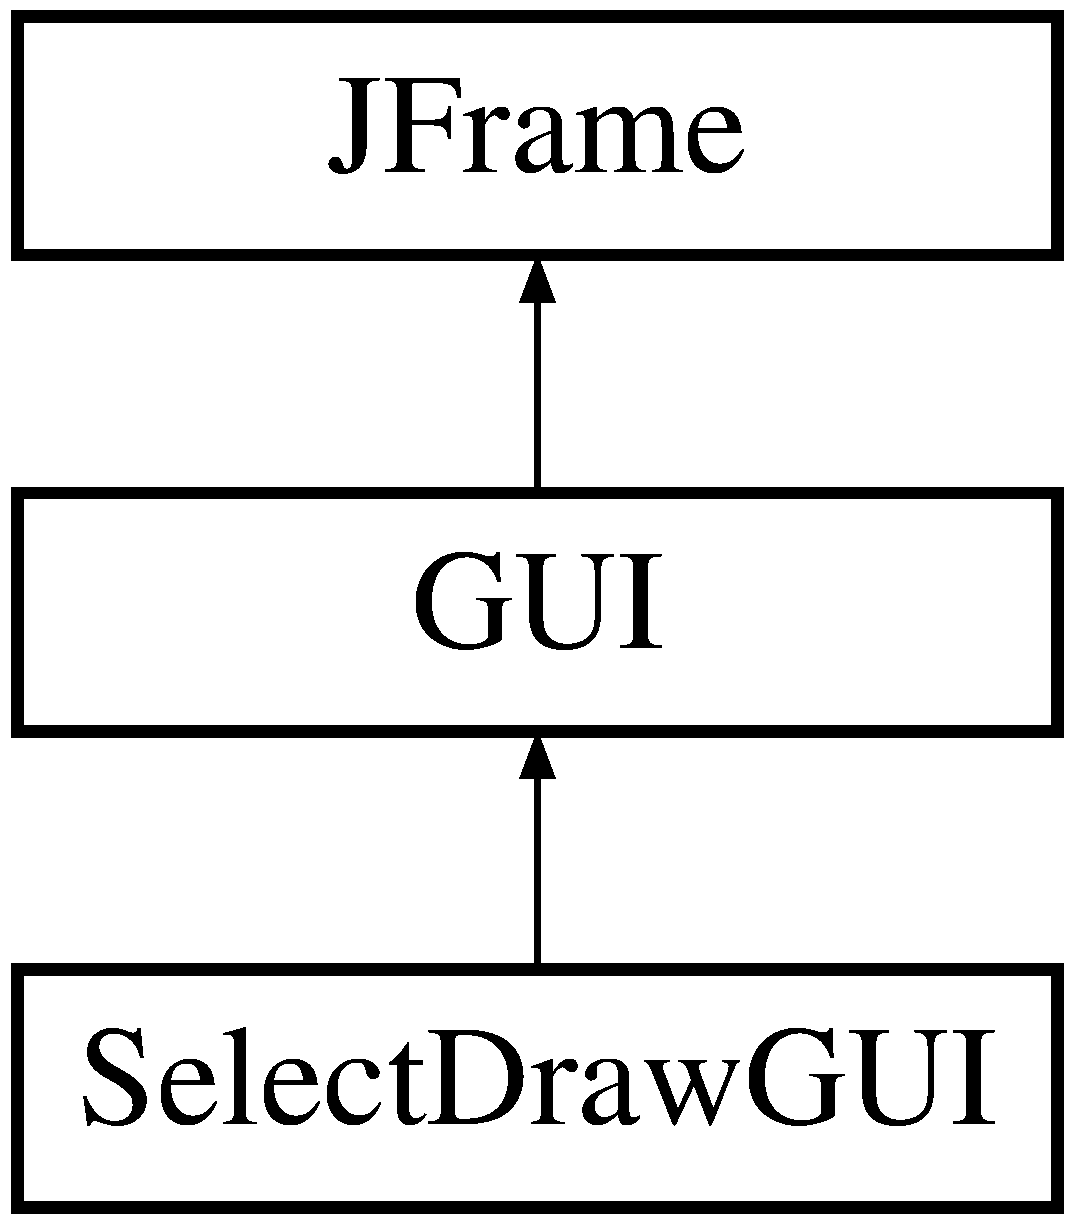
\includegraphics[height=3.000000cm]{class_select_draw_g_u_i}
\end{center}
\end{figure}
\subsection*{Public Member Functions}
\begin{DoxyCompactItemize}
\item 
\hyperlink{class_select_draw_g_u_i_a5437524cbdb011b9afd066ed51a8830d}{Select\+Draw\+G\+UI} (\hyperlink{class_account}{Account} acc)  throws Exception 
\begin{DoxyCompactList}\small\item\em Builds the screen and implements action listeners. \end{DoxyCompactList}\end{DoxyCompactItemize}
\subsection*{Static Public Member Functions}
\begin{DoxyCompactItemize}
\item 
\mbox{\Hypertarget{class_select_draw_g_u_i_abb206d6887f59cabc6f1b0c16cdb2522}\label{class_select_draw_g_u_i_abb206d6887f59cabc6f1b0c16cdb2522}} 
static void \hyperlink{class_select_draw_g_u_i_abb206d6887f59cabc6f1b0c16cdb2522}{main} (String\mbox{[}$\,$\mbox{]} args)  throws Exception 	
\begin{DoxyCompactList}\small\item\em Implemented for testing purposes. \end{DoxyCompactList}\end{DoxyCompactItemize}


\subsection{Constructor \& Destructor Documentation}
\mbox{\Hypertarget{class_select_draw_g_u_i_a5437524cbdb011b9afd066ed51a8830d}\label{class_select_draw_g_u_i_a5437524cbdb011b9afd066ed51a8830d}} 
\index{Select\+Draw\+G\+UI@{Select\+Draw\+G\+UI}!Select\+Draw\+G\+UI@{Select\+Draw\+G\+UI}}
\index{Select\+Draw\+G\+UI@{Select\+Draw\+G\+UI}!Select\+Draw\+G\+UI@{Select\+Draw\+G\+UI}}
\subsubsection{\texorpdfstring{Select\+Draw\+G\+U\+I()}{SelectDrawGUI()}}
{\footnotesize\ttfamily Select\+Draw\+G\+U\+I.\+Select\+Draw\+G\+UI (\begin{DoxyParamCaption}\item[{\hyperlink{class_account}{Account}}]{acc }\end{DoxyParamCaption}) throws Exception}



Builds the screen and implements action listeners. 


\begin{DoxyParams}{Parameters}
{\em acc} & Reference to the currently logged in \hyperlink{class_account}{Account} \\
\hline
\end{DoxyParams}


The documentation for this class was generated from the following file\+:\begin{DoxyCompactItemize}
\item 
readwrite/Select\+Draw\+G\+U\+I.\+java\end{DoxyCompactItemize}

\hypertarget{class_text_message}{}\section{Text\+Message Class Reference}
\label{class_text_message}\index{Text\+Message@{Text\+Message}}


Text\+Message.\+java.  


Inheritance diagram for Text\+Message\+:\begin{figure}[H]
\begin{center}
\leavevmode
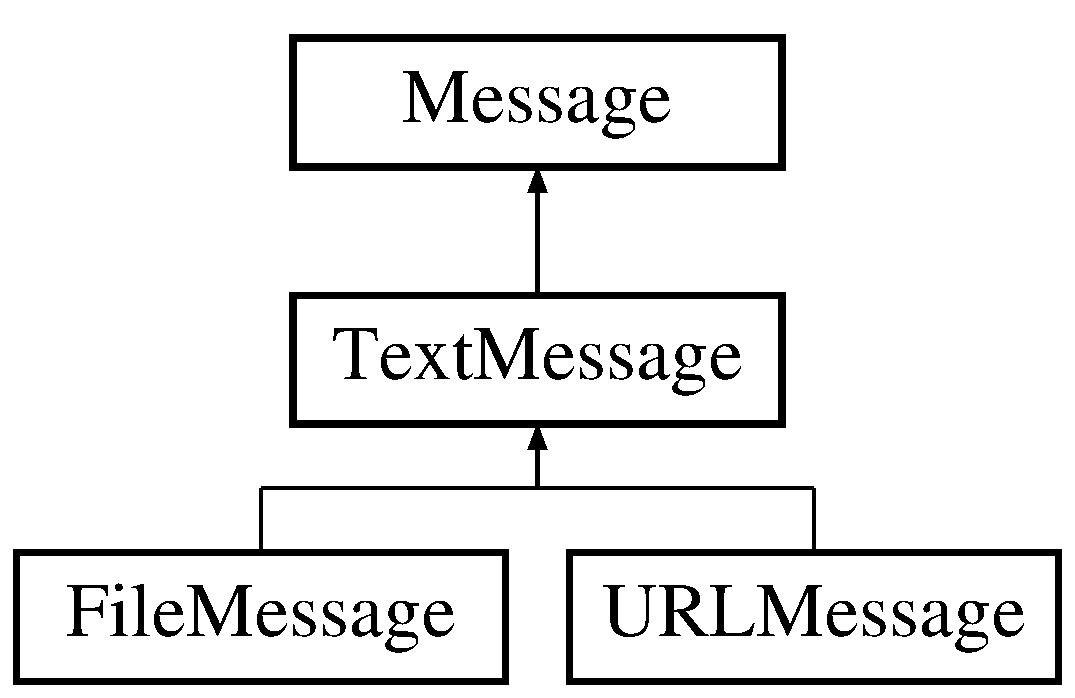
\includegraphics[height=3.000000cm]{class_text_message}
\end{center}
\end{figure}
\subsection*{Public Member Functions}
\begin{DoxyCompactItemize}
\item 
\mbox{\Hypertarget{class_text_message_a5836488ebd4cf272973a9d86aba5b947}\label{class_text_message_a5836488ebd4cf272973a9d86aba5b947}} 
{\bfseries Text\+Message} (String recipient, String sender, String message\+Content)
\item 
\mbox{\Hypertarget{class_text_message_a7cfe165a3ad870ae2b1979ba1c2f7b6c}\label{class_text_message_a7cfe165a3ad870ae2b1979ba1c2f7b6c}} 
void {\bfseries set\+Message\+Content} (String message\+Content)
\item 
\mbox{\Hypertarget{class_text_message_a2ab60ed6752642092be32157d01689d8}\label{class_text_message_a2ab60ed6752642092be32157d01689d8}} 
String {\bfseries get\+Message\+Content} ()
\item 
\mbox{\Hypertarget{class_text_message_a2984283095d6e8e6d91460264b831366}\label{class_text_message_a2984283095d6e8e6d91460264b831366}} 
void {\bfseries send\+Message} ()
\end{DoxyCompactItemize}
\subsection*{Static Public Member Functions}
\begin{DoxyCompactItemize}
\item 
\mbox{\Hypertarget{class_text_message_a2eafe943799343f3613eec8ef11e6b58}\label{class_text_message_a2eafe943799343f3613eec8ef11e6b58}} 
static void \hyperlink{class_text_message_a2eafe943799343f3613eec8ef11e6b58}{main} (String\mbox{[}$\,$\mbox{]} args)
\begin{DoxyCompactList}\small\item\em Implemented for testing purposes. \end{DoxyCompactList}\end{DoxyCompactItemize}


\subsection{Detailed Description}
Text\+Message.\+java. 

\begin{DoxyAuthor}{Author}
Wenju Mu, Dan Woolsey
\end{DoxyAuthor}
Class to construct a \hyperlink{class_text_message}{Text\+Message} object 

The documentation for this class was generated from the following file\+:\begin{DoxyCompactItemize}
\item 
readwrite/Text\+Message.\+java\end{DoxyCompactItemize}

\hypertarget{class_upload_g_u_i}{}\section{Upload\+G\+UI Class Reference}
\label{class_upload_g_u_i}\index{Upload\+G\+UI@{Upload\+G\+UI}}
Inheritance diagram for Upload\+G\+UI\+:\begin{figure}[H]
\begin{center}
\leavevmode
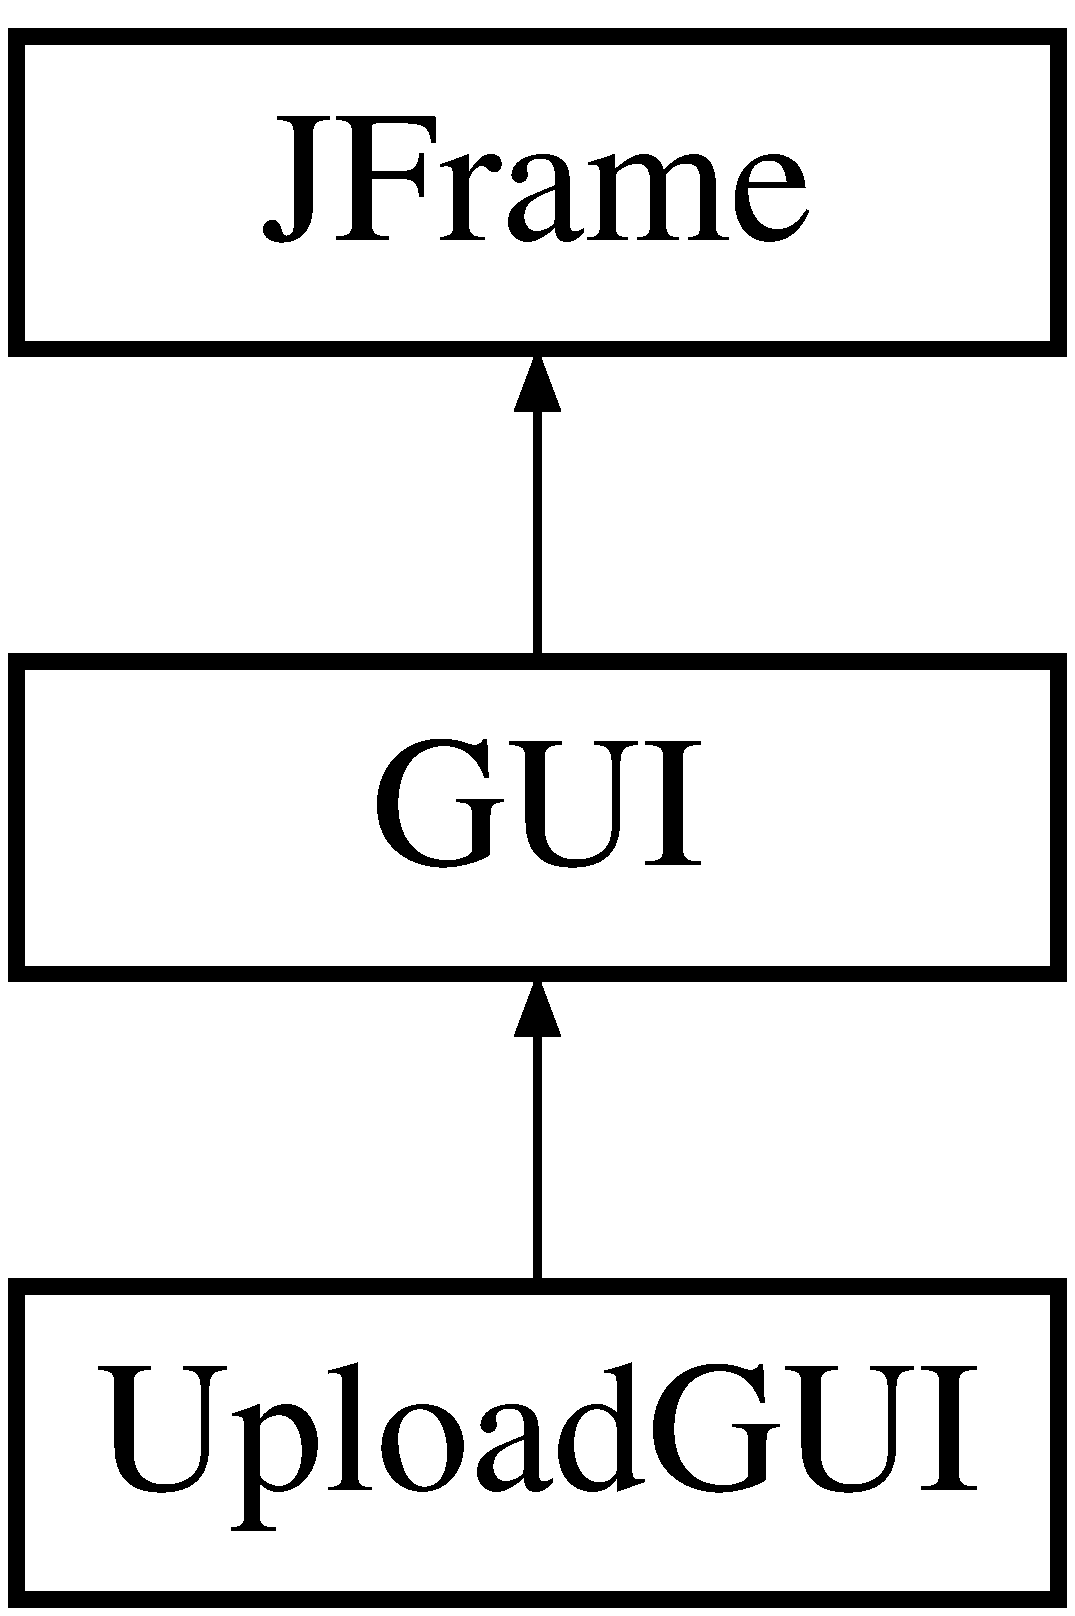
\includegraphics[height=3.000000cm]{class_upload_g_u_i}
\end{center}
\end{figure}
\subsection*{Public Member Functions}
\begin{DoxyCompactItemize}
\item 
\hyperlink{class_upload_g_u_i_a19f2e3a86156809d4497a210b508ede2}{Upload\+G\+UI} (\hyperlink{class_account}{Account} acc)  throws Exception
\item 
void \hyperlink{class_upload_g_u_i_a4f67dc6bcb1ae96c2b7a148918348075}{uploadsetup} (\hyperlink{class_account}{Account} acc)  throws Exception
\begin{DoxyCompactList}\small\item\em Sets up the window and action listener. \end{DoxyCompactList}\end{DoxyCompactItemize}
\subsection*{Static Public Member Functions}
\begin{DoxyCompactItemize}
\item 
\mbox{\Hypertarget{class_upload_g_u_i_a01ff7bc7e4b088ed35f11359ef713caa}\label{class_upload_g_u_i_a01ff7bc7e4b088ed35f11359ef713caa}} 
static void \hyperlink{class_upload_g_u_i_a01ff7bc7e4b088ed35f11359ef713caa}{main} (String\mbox{[}$\,$\mbox{]} args)  throws Exception
\begin{DoxyCompactList}\small\item\em Implemented for testing purposes. \end{DoxyCompactList}\end{DoxyCompactItemize}


\subsection{Constructor \& Destructor Documentation}
\mbox{\Hypertarget{class_upload_g_u_i_a19f2e3a86156809d4497a210b508ede2}\label{class_upload_g_u_i_a19f2e3a86156809d4497a210b508ede2}} 
\index{Upload\+G\+UI@{Upload\+G\+UI}!Upload\+G\+UI@{Upload\+G\+UI}}
\index{Upload\+G\+UI@{Upload\+G\+UI}!Upload\+G\+UI@{Upload\+G\+UI}}
\subsubsection{\texorpdfstring{Upload\+G\+U\+I()}{UploadGUI()}}
{\footnotesize\ttfamily Upload\+G\+U\+I.\+Upload\+G\+UI (\begin{DoxyParamCaption}\item[{\hyperlink{class_account}{Account}}]{acc }\end{DoxyParamCaption}) throws Exception}


\begin{DoxyParams}{Parameters}
{\em acc} & Reference to the \hyperlink{class_account}{Account} current logged in \\
\hline
\end{DoxyParams}


\subsection{Member Function Documentation}
\mbox{\Hypertarget{class_upload_g_u_i_a4f67dc6bcb1ae96c2b7a148918348075}\label{class_upload_g_u_i_a4f67dc6bcb1ae96c2b7a148918348075}} 
\index{Upload\+G\+UI@{Upload\+G\+UI}!uploadsetup@{uploadsetup}}
\index{uploadsetup@{uploadsetup}!Upload\+G\+UI@{Upload\+G\+UI}}
\subsubsection{\texorpdfstring{uploadsetup()}{uploadsetup()}}
{\footnotesize\ttfamily void Upload\+G\+U\+I.\+uploadsetup (\begin{DoxyParamCaption}\item[{\hyperlink{class_account}{Account}}]{acc }\end{DoxyParamCaption}) throws Exception}



Sets up the window and action listener. 


\begin{DoxyParams}{Parameters}
{\em acc} & reference to the currently logged in \hyperlink{class_account}{Account} \\
\hline
\end{DoxyParams}


The documentation for this class was generated from the following file\+:\begin{DoxyCompactItemize}
\item 
readwrite/Upload\+G\+U\+I.\+java\end{DoxyCompactItemize}

\hypertarget{class_u_r_l_message}{}\section{U\+R\+L\+Message Class Reference}
\label{class_u_r_l_message}\index{U\+R\+L\+Message@{U\+R\+L\+Message}}
Inheritance diagram for U\+R\+L\+Message\+:\begin{figure}[H]
\begin{center}
\leavevmode
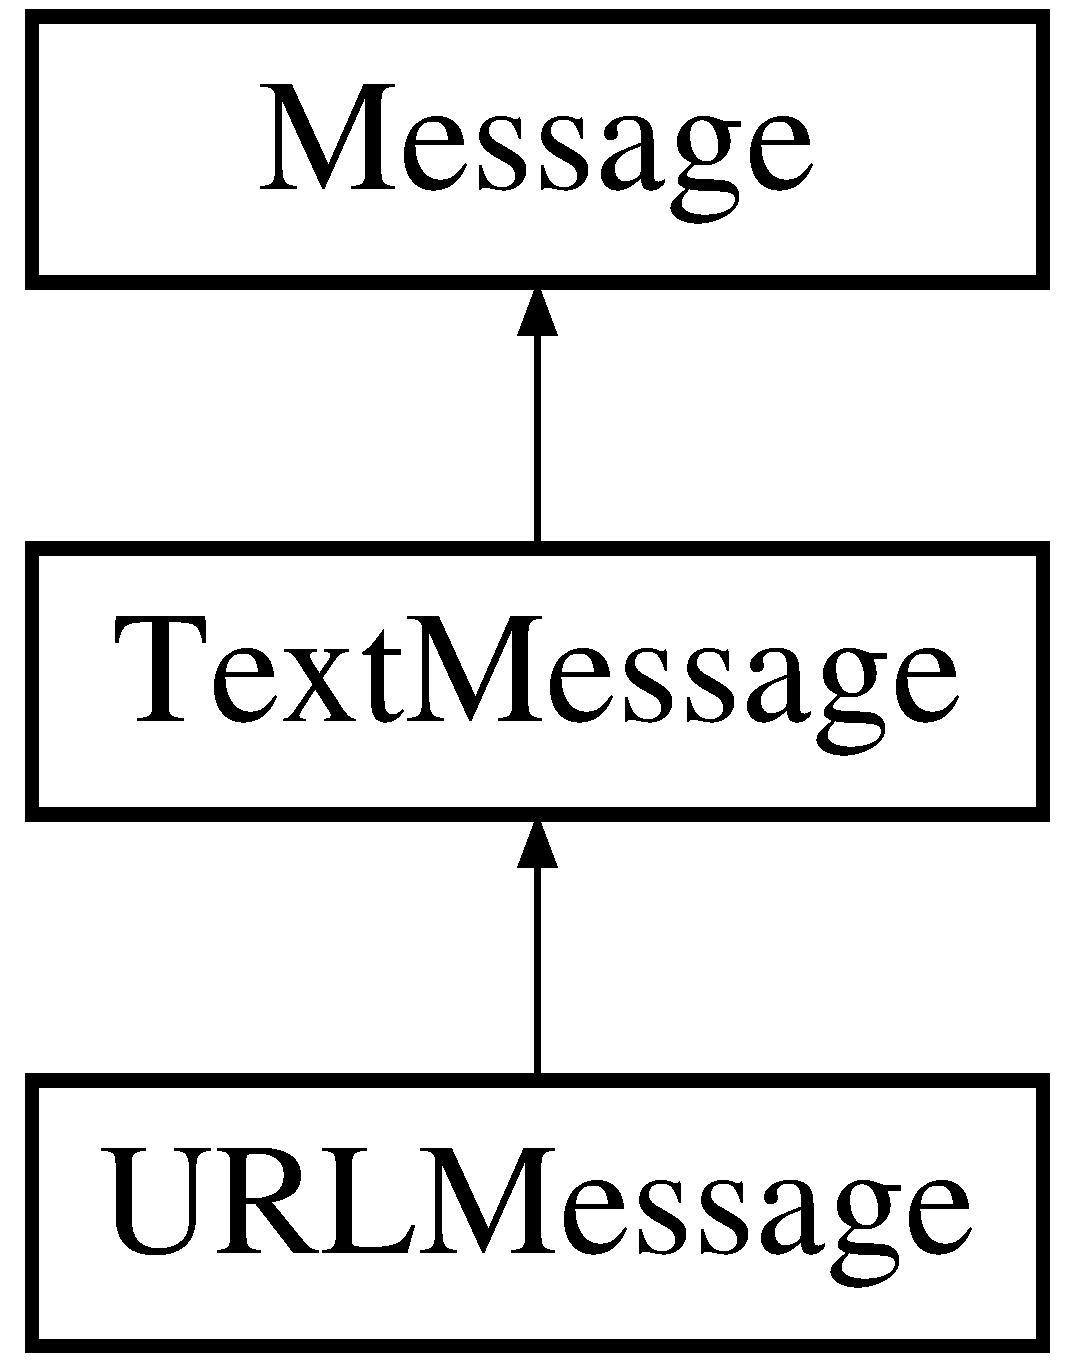
\includegraphics[height=3.000000cm]{class_u_r_l_message}
\end{center}
\end{figure}
\subsection*{Public Member Functions}
\begin{DoxyCompactItemize}
\item 
\mbox{\Hypertarget{class_u_r_l_message_a277e910970a76bf04a5c64ad7d41c0b6}\label{class_u_r_l_message_a277e910970a76bf04a5c64ad7d41c0b6}} 
\hyperlink{class_u_r_l_message_a277e910970a76bf04a5c64ad7d41c0b6}{U\+R\+L\+Message} (String recipient, String sender, String msg, String url)
\begin{DoxyCompactList}\small\item\em Create a \hyperlink{class_u_r_l_message}{U\+R\+L\+Message}. \end{DoxyCompactList}\item 
void \hyperlink{class_u_r_l_message_a2056536ac32514f5f41ba8c6b4e4f66d}{set\+\_\+url} (String url)
\item 
String \hyperlink{class_u_r_l_message_a9c2a3498360de3e3cc50cfe91b732f11}{get\+U\+RL} ()
\item 
\mbox{\Hypertarget{class_u_r_l_message_a403528f2856ab482e8b532de0cb9d68f}\label{class_u_r_l_message_a403528f2856ab482e8b532de0cb9d68f}} 
void \hyperlink{class_u_r_l_message_a403528f2856ab482e8b532de0cb9d68f}{open\+U\+RL} ()
\begin{DoxyCompactList}\small\item\em Opens the url embedded in the message with the users default browser. \end{DoxyCompactList}\item 
\mbox{\Hypertarget{class_u_r_l_message_a35cd7dac3ad9536b90f46c80f0aa92bf}\label{class_u_r_l_message_a35cd7dac3ad9536b90f46c80f0aa92bf}} 
void {\bfseries send\+Message} ()
\end{DoxyCompactItemize}
\subsection*{Static Public Member Functions}
\begin{DoxyCompactItemize}
\item 
\mbox{\Hypertarget{class_u_r_l_message_a2337e1bf5b85d8b18f0bd99fc68a5193}\label{class_u_r_l_message_a2337e1bf5b85d8b18f0bd99fc68a5193}} 
static void \hyperlink{class_u_r_l_message_a2337e1bf5b85d8b18f0bd99fc68a5193}{main} (String\mbox{[}$\,$\mbox{]} args)
\begin{DoxyCompactList}\small\item\em In place for testing purposes. \end{DoxyCompactList}\end{DoxyCompactItemize}


\subsection{Member Function Documentation}
\mbox{\Hypertarget{class_u_r_l_message_a9c2a3498360de3e3cc50cfe91b732f11}\label{class_u_r_l_message_a9c2a3498360de3e3cc50cfe91b732f11}} 
\index{U\+R\+L\+Message@{U\+R\+L\+Message}!get\+U\+RL@{get\+U\+RL}}
\index{get\+U\+RL@{get\+U\+RL}!U\+R\+L\+Message@{U\+R\+L\+Message}}
\subsubsection{\texorpdfstring{get\+U\+R\+L()}{getURL()}}
{\footnotesize\ttfamily String U\+R\+L\+Message.\+get\+U\+RL (\begin{DoxyParamCaption}{ }\end{DoxyParamCaption})}

\begin{DoxyReturn}{Returns}
String of the embedded U\+RL 
\end{DoxyReturn}
\mbox{\Hypertarget{class_u_r_l_message_a2056536ac32514f5f41ba8c6b4e4f66d}\label{class_u_r_l_message_a2056536ac32514f5f41ba8c6b4e4f66d}} 
\index{U\+R\+L\+Message@{U\+R\+L\+Message}!set\+\_\+url@{set\+\_\+url}}
\index{set\+\_\+url@{set\+\_\+url}!U\+R\+L\+Message@{U\+R\+L\+Message}}
\subsubsection{\texorpdfstring{set\+\_\+url()}{set\_url()}}
{\footnotesize\ttfamily void U\+R\+L\+Message.\+set\+\_\+url (\begin{DoxyParamCaption}\item[{String}]{url }\end{DoxyParamCaption})}


\begin{DoxyParams}{Parameters}
{\em url} & new U\+RL \\
\hline
\end{DoxyParams}


The documentation for this class was generated from the following file\+:\begin{DoxyCompactItemize}
\item 
readwrite/U\+R\+L\+Message.\+java\end{DoxyCompactItemize}

\hypertarget{class_vertex}{}\section{Vertex Class Reference}
\label{class_vertex}\index{Vertex@{Vertex}}


The \hyperlink{class_vertex}{Vertex} class will be used in the \hyperlink{class_graph}{Graph} and \hyperlink{class_edge}{Edge} classes.  


\subsection*{Public Member Functions}
\begin{DoxyCompactItemize}
\item 
\hyperlink{class_vertex_a55f0a6d7d075b9d1881ebaaea3859970}{Vertex} (String username)
\begin{DoxyCompactList}\small\item\em constructor for a vertex \end{DoxyCompactList}\item 
void \hyperlink{class_vertex_a77dbe86276566b77bdb2d631472660cf}{add\+Edge} (\hyperlink{class_edge}{Edge} edge)
\begin{DoxyCompactList}\small\item\em add an edge to the vertex\textquotesingle{}s arraylist of edges that its involved in \end{DoxyCompactList}\item 
boolean \hyperlink{class_vertex_a4a77d1c66be46bef636154798bb3b96d}{contains\+Edge} (\hyperlink{class_edge}{Edge} edge)
\begin{DoxyCompactList}\small\item\em check if the edges arraylist contains a certain edge \end{DoxyCompactList}\item 
\hyperlink{class_edge}{Edge} \hyperlink{class_vertex_a428fe1ef66c8422b3af1aa4566360f13}{get\+Edge} (int index)
\begin{DoxyCompactList}\small\item\em return the edge at specified index \end{DoxyCompactList}\item 
void \hyperlink{class_vertex_a74032add8df85233c3979374471a3141}{remove\+Edge} (\hyperlink{class_edge}{Edge} edge)
\begin{DoxyCompactList}\small\item\em remove edge from the arraylist \end{DoxyCompactList}\item 
int \hyperlink{class_vertex_a3da0cb5ceb6e70ffbdfd84941fa69b4a}{get\+Number\+Edges} ()
\begin{DoxyCompactList}\small\item\em get number of edges \end{DoxyCompactList}\item 
String \hyperlink{class_vertex_a24b931258451256742b50b09b5a8e13f}{get\+Username} ()
\begin{DoxyCompactList}\small\item\em returns the username of vertex \end{DoxyCompactList}\item 
Array\+List$<$ \hyperlink{class_edge}{Edge} $>$ \hyperlink{class_vertex_a25a9ddc7d963c1f7a762d8f6b68376dc}{get\+Edges} ()
\begin{DoxyCompactList}\small\item\em return arraylist of edges for this vertex \end{DoxyCompactList}\end{DoxyCompactItemize}


\subsection{Detailed Description}
The \hyperlink{class_vertex}{Vertex} class will be used in the \hyperlink{class_graph}{Graph} and \hyperlink{class_edge}{Edge} classes. 

It also uses the \hyperlink{class_edge}{Edge} class. A vertex has a username to identify it by, and an arraylist of edges that it is involved in

\begin{DoxyAuthor}{Author}
830169 
\end{DoxyAuthor}
\begin{DoxyVersion}{Version}
1.\+0 
\end{DoxyVersion}


\subsection{Constructor \& Destructor Documentation}
\mbox{\Hypertarget{class_vertex_a55f0a6d7d075b9d1881ebaaea3859970}\label{class_vertex_a55f0a6d7d075b9d1881ebaaea3859970}} 
\index{Vertex@{Vertex}!Vertex@{Vertex}}
\index{Vertex@{Vertex}!Vertex@{Vertex}}
\subsubsection{\texorpdfstring{Vertex()}{Vertex()}}
{\footnotesize\ttfamily Vertex.\+Vertex (\begin{DoxyParamCaption}\item[{String}]{username }\end{DoxyParamCaption})}



constructor for a vertex 


\begin{DoxyParams}{Parameters}
{\em username} & the username that corresponds to the vertex \\
\hline
\end{DoxyParams}


\subsection{Member Function Documentation}
\mbox{\Hypertarget{class_vertex_a77dbe86276566b77bdb2d631472660cf}\label{class_vertex_a77dbe86276566b77bdb2d631472660cf}} 
\index{Vertex@{Vertex}!add\+Edge@{add\+Edge}}
\index{add\+Edge@{add\+Edge}!Vertex@{Vertex}}
\subsubsection{\texorpdfstring{add\+Edge()}{addEdge()}}
{\footnotesize\ttfamily void Vertex.\+add\+Edge (\begin{DoxyParamCaption}\item[{\hyperlink{class_edge}{Edge}}]{edge }\end{DoxyParamCaption})}



add an edge to the vertex\textquotesingle{}s arraylist of edges that its involved in 


\begin{DoxyParams}{Parameters}
{\em edge} & the edge to add \\
\hline
\end{DoxyParams}
\mbox{\Hypertarget{class_vertex_a4a77d1c66be46bef636154798bb3b96d}\label{class_vertex_a4a77d1c66be46bef636154798bb3b96d}} 
\index{Vertex@{Vertex}!contains\+Edge@{contains\+Edge}}
\index{contains\+Edge@{contains\+Edge}!Vertex@{Vertex}}
\subsubsection{\texorpdfstring{contains\+Edge()}{containsEdge()}}
{\footnotesize\ttfamily boolean Vertex.\+contains\+Edge (\begin{DoxyParamCaption}\item[{\hyperlink{class_edge}{Edge}}]{edge }\end{DoxyParamCaption})}



check if the edges arraylist contains a certain edge 


\begin{DoxyParams}{Parameters}
{\em edge} & the edge being searched for \\
\hline
\end{DoxyParams}
\begin{DoxyReturn}{Returns}
returns true if the edge exists 
\end{DoxyReturn}
\mbox{\Hypertarget{class_vertex_a428fe1ef66c8422b3af1aa4566360f13}\label{class_vertex_a428fe1ef66c8422b3af1aa4566360f13}} 
\index{Vertex@{Vertex}!get\+Edge@{get\+Edge}}
\index{get\+Edge@{get\+Edge}!Vertex@{Vertex}}
\subsubsection{\texorpdfstring{get\+Edge()}{getEdge()}}
{\footnotesize\ttfamily \hyperlink{class_edge}{Edge} Vertex.\+get\+Edge (\begin{DoxyParamCaption}\item[{int}]{index }\end{DoxyParamCaption})}



return the edge at specified index 


\begin{DoxyParams}{Parameters}
{\em index} & the index of the arraylist that the edge is located at \\
\hline
\end{DoxyParams}
\begin{DoxyReturn}{Returns}
returns an edge 
\end{DoxyReturn}
\mbox{\Hypertarget{class_vertex_a25a9ddc7d963c1f7a762d8f6b68376dc}\label{class_vertex_a25a9ddc7d963c1f7a762d8f6b68376dc}} 
\index{Vertex@{Vertex}!get\+Edges@{get\+Edges}}
\index{get\+Edges@{get\+Edges}!Vertex@{Vertex}}
\subsubsection{\texorpdfstring{get\+Edges()}{getEdges()}}
{\footnotesize\ttfamily Array\+List$<$\hyperlink{class_edge}{Edge}$>$ Vertex.\+get\+Edges (\begin{DoxyParamCaption}{ }\end{DoxyParamCaption})}



return arraylist of edges for this vertex 

\begin{DoxyReturn}{Returns}
arraylist containing all edges this vertex is involved in 
\end{DoxyReturn}
\mbox{\Hypertarget{class_vertex_a3da0cb5ceb6e70ffbdfd84941fa69b4a}\label{class_vertex_a3da0cb5ceb6e70ffbdfd84941fa69b4a}} 
\index{Vertex@{Vertex}!get\+Number\+Edges@{get\+Number\+Edges}}
\index{get\+Number\+Edges@{get\+Number\+Edges}!Vertex@{Vertex}}
\subsubsection{\texorpdfstring{get\+Number\+Edges()}{getNumberEdges()}}
{\footnotesize\ttfamily int Vertex.\+get\+Number\+Edges (\begin{DoxyParamCaption}{ }\end{DoxyParamCaption})}



get number of edges 

\begin{DoxyReturn}{Returns}
the number of edges this vertex is involved in 
\end{DoxyReturn}
\mbox{\Hypertarget{class_vertex_a24b931258451256742b50b09b5a8e13f}\label{class_vertex_a24b931258451256742b50b09b5a8e13f}} 
\index{Vertex@{Vertex}!get\+Username@{get\+Username}}
\index{get\+Username@{get\+Username}!Vertex@{Vertex}}
\subsubsection{\texorpdfstring{get\+Username()}{getUsername()}}
{\footnotesize\ttfamily String Vertex.\+get\+Username (\begin{DoxyParamCaption}{ }\end{DoxyParamCaption})}



returns the username of vertex 

\begin{DoxyReturn}{Returns}
username of the vertex 
\end{DoxyReturn}
\mbox{\Hypertarget{class_vertex_a74032add8df85233c3979374471a3141}\label{class_vertex_a74032add8df85233c3979374471a3141}} 
\index{Vertex@{Vertex}!remove\+Edge@{remove\+Edge}}
\index{remove\+Edge@{remove\+Edge}!Vertex@{Vertex}}
\subsubsection{\texorpdfstring{remove\+Edge()}{removeEdge()}}
{\footnotesize\ttfamily void Vertex.\+remove\+Edge (\begin{DoxyParamCaption}\item[{\hyperlink{class_edge}{Edge}}]{edge }\end{DoxyParamCaption})}



remove edge from the arraylist 


\begin{DoxyParams}{Parameters}
{\em edge} & edge to be removed \\
\hline
\end{DoxyParams}


The documentation for this class was generated from the following file\+:\begin{DoxyCompactItemize}
\item 
readwrite/Vertex.\+java\end{DoxyCompactItemize}

\chapter{File Documentation}
\hypertarget{_home_g_u_i_8java}{}\section{readwrite/\+Home\+G\+UI.java File Reference}
\label{_home_g_u_i_8java}\index{readwrite/\+Home\+G\+U\+I.\+java@{readwrite/\+Home\+G\+U\+I.\+java}}


Home screen for the Skypertawe application.  


\subsection*{Classes}
\begin{DoxyCompactItemize}
\item 
class \hyperlink{class_home_g_u_i}{Home\+G\+UI}
\end{DoxyCompactItemize}


\subsection{Detailed Description}
Home screen for the Skypertawe application. 

\begin{DoxyAuthor}{Author}
Stefan Ficur, Dan Woolsey 
\end{DoxyAuthor}

%--- End generated contents ---

% Index
\backmatter
\newpage
\phantomsection
\clearemptydoublepage
\addcontentsline{toc}{chapter}{Index}
\printindex

\end{document}
